\documentclass[11pt, openany]{report}
\usepackage[utf8]{inputenc}
\usepackage[T1]{fontenc}
\usepackage[a4paper,left=3cm,right=3cm,top=3cm,bottom=3cm]{geometry}
\usepackage[english]{babel}
\usepackage{libertine}
\usepackage[pdftex]{graphicx}
\usepackage{tabu}
\usepackage{makeidx}
\usepackage{lipsum}
\makeindex

\setlength{\parindent}{0cm}
\setlength{\parskip}{1ex plus 0.5ex minus 0.2ex}
\newcommand{\hsp}{\hspace{20pt}}
\newcommand{\HRule}{\rule{\linewidth}{0.5mm}}
\usepackage[dvipsnames]{xcolor}

\usepackage{amsmath,amsfonts,amssymb,amsthm,epsfig,epstopdf,titling,url,array}

% SHOW SUBSUBSECTION IN TABLES OF CONTENTS 
\setcounter{tocdepth}{3}
\setcounter{secnumdepth}{3}

% BIBLIOGRAPHIE 
\usepackage{natbib}
\bibliographystyle{apalike-fr}
\renewcommand{\UrlFont}{\ttfamily\footnotesize}

% CAPTION PACKAGE
\usepackage{caption}
\usepackage[hidelinks]{hyperref}
\usepackage{xcolor}
\usepackage{makecell}

%%% MATHS PACKAGE 
\theoremstyle{plain}
\newtheorem{thm}{Theorem}[section]
\newtheorem{lem}[thm]{Lemma}
\newtheorem{prop}[thm]{Proposition}
\newtheorem*{cor}{Corollary}
\newcommand\norm[1]{\left\lVert#1\right\rVert}

%ALGORITHM
\usepackage{algorithm}
\usepackage[noend]{algpseudocode}
\renewcommand{\algorithmicforall}{\textbf{for each}}
\newcommand{\var}[1]{\mathit{#1}}
\newcommand{\func}[1]{\mathrm{#1}}
\algdef{SE}[DOWHILE]{Do}{doWhile}{\algorithmicdo}[1]{\algorithmicwhile\ #1}
%

\theoremstyle{definition}
\newtheorem{defn}{Definition}[section]
\newtheorem{conj}{Conjecture}[section]
\newtheorem{exmp}{Example}[section]

\theoremstyle{remark}
\newtheorem*{rem}{Remark}
\newtheorem*{note}{Note}

\usepackage[scaled=.8]{beramono}

\DeclareUnicodeCharacter{200A}{!!!FIX ME!!!} 

\begin{document}

%%%%%%%%%%%%%%%%%%%%%%%% PAGE DE GARDE %%%%%%%%%%%%%%%%%%%%%%%%
\begin{titlepage}
  \begin{sffamily}
  \begin{center}

    % Upper part of the page. The '~' is needed because \\
    % only works if a paragraph has started.
    
\includegraphics[scale=0.4]{figures/logo_ulb.jpg}~\\[1cm]
    
	\textsc{\LARGE UNIVERSITÉ LIBRE DE BRUXELLES}\\[0.5cm]
    \textsc{\LARGE Computer Sciences Department, Faculty of Sciences}\\[2cm]
    \textsc{\LARGE Computer Sciences Master Thesis}\\[2cm]

    % Title
    \hrule width 15cm
    \vspace{0.5cm}
    { \huge \bfseries Methods for large-scale image classification and application to biomedical data}
    \vspace{0.5cm}
	\hrule width 15cm
	\vspace{1cm}
	
	
	\LARGE Quang Linh \textsc{\textbf{\LARGE Bui Quang Phuong}} \\ [0.5cm]
	\large ULB ID: 000427796 
	
    \vfill

    % Bottom of the page
    {\large \textbf{Promotor :} Matthieu Defrance} \\
    \vspace{0.5cm}
    Academic Year 2019-2020

  \end{center}
  \end{sffamily}
\end{titlepage}


\begin{abstract}

In this document, the important computer vision problem called image classification is tackled. To introduce the problem, different applications of image recognition and classification are given and explained to prove its importance in our actual world,  especially in the medical field which will be focused in this paper. Furthermore, machine learning and deep learning methods are used to solve image classification problem. In 2012, convolutional neural networks (CNN) have significantly increase the performance of the previous learning methods. In addition to CNN, this document expounds support vector machines (SVM) which is a well-known method for classifying data into classes. Subsequently, these methods will be used to resolve medical images classification problems. In particular, the methodology following Regab et al.'s paper \cite{breast-cancer} to detect breast cancer by analysing mammogram images with an average accuracy of 80\%  makes subject of an entire chapter of the document.      

\end{abstract}

%%%%%%%%%%%%%%%%%%%%%%%% TABLE DES MATIERES %%%%%%%%%%%%%%%%%%%%%%%%
\tableofcontents


\chapter{Introduction}

\section{Context and birth of the classification problem}

\subsection{Context}

In our days, countless numbers of pictures are taken of everything and anything due to the exponential growing of photography and digital photo cameras. Whether it is thanks to the built-in camera of your smartphone or your faithful travel companion, taking a picture has become a disconcerting ease. All these pictures are inevitably shared and searched on the internet. Without any classification, it would be a really laborious task to find a particular picture over the millions (even billions actually!) photos taken by users worldwide. This classification problem can be extended in a large panel of fields: it can go from your personal use to a more impacting field such as medical images analysis. Overall, this problem can be generalized and divided into an image processing and recognition sub-problems. More applications are presented in the next section.  \\

Thereby, fast and efficient methods have to be found to realize a reliable classification of big data. It is in the 50's, when the artificial intelligence (AI) has begun to take shape, that image recognition becomes a more serious problem to manage. As Marvin Minsky, co-founder of the Massachusetts Institute of Technology's (MIT) AI laboratory, defines: 
\begin{quote}
\textit{"AI is the science of making machines do things that would require intelligence if done by men."} (1968)
\end{quote}      

Following this definition, image recognition and classification can clearly be resolved by AI methods, such as \textit{Machine Learning} -- which is a technique for teaching machines to learn, and indeed becomes one of the main application of AI. \\

\subsection{History and first methods}

The first methods used are based on \textit{Artificial Neural Networks} (ANN) where the first artificial neuron is created in 1943. Very briefly, the basic idea behind a neural network is to simulate (i.e. copy in a good way) lots of densely interconnected brain cells inside a computer so you can get it to learn things and recognize patterns to finally take a decision as a human would do. % source:https://www.explainthatstuff.com/introduction-to-neural-networks.html
This is exactly what we want to apply for an image. Giving on input an image, the neural network will recognize and learn the different patterns of this input and will assign the image on a specific category where these patterns are retrieved. These patterns are also called \textbf{features}.

Nevertheless, it is in the 21st century that image classification and recognition has evolved faster and faster. Previously, the accuracy of the recognition was not very high, implying a somehow large rate of error (at least more than 20\%).

In 2010, the appearance of \textit{Deep Learning} -- a class of machine learning algorithms that goes deeper into data to recognize patterns, accelerates the evolution of image classification problem and enhances this accuracy, especially due to a new class of neural networks called \textit{Convolutional Neural Networks} (CNN) that will be tackled in details in the next chapters.  % à expliquer vite fait 

For instance, in 2012, Alex Krizhevsky, Ilya Sutskever and Geoffrey Hinton created a new recognition algorithm for objects images ensuring an 85\% level of accuracy and in 2015, developed tools using CNN reaches a 95\% level of accuracy for facial recognition \cite{History-1}. \\  

\section{Some application of image classification}
% lien utile : https://imagga.com/blog/the-top-5-uses-of-image-recognition/

\subsection{Google Images}
When thinking of image classification, Google Images is probably one of the most famous application of image classification. This extension of Google is the most used image search engine. At the beginning, Google's technology do basic things like extracting text from images, but its real power is in actually recognizing the objects in an image. Google says it has trained the algorithm to recognize "thousands" of different objects. % source: https://techcrunch.com/2016/02/18/google-opens-its-cloud-vision-api-to-all-developers/?guccounter=1
Over time, Google has evolved and offers new features analysis such as sentiment and emotion detection. \\

Moreover, in 2013, Google released search for personal photos, giving users the ability to retrieve photos in their libraries based on the objects present in the images. Two years later, in 2015, this feature was implemented in Google Photos, the application of Google that stores all of your personal photos to ease your photos classification \cite{Google-2}. Following the AI's definition of Minsky, that proves that computer vision software could classify images to human standards avoiding annoying tasks to humans such as labelling manually all its photos. The models built to label images are even done to see pictures more like humans do. Indeed, the model is analysing every pixel of the photo and does not take in account if the object is in the foreground or in the background, the model will label it anyway as seen in the example given in \autoref{fig:googleImages-ex-labelling}. 

\begin{figure}[h]
  \centering
  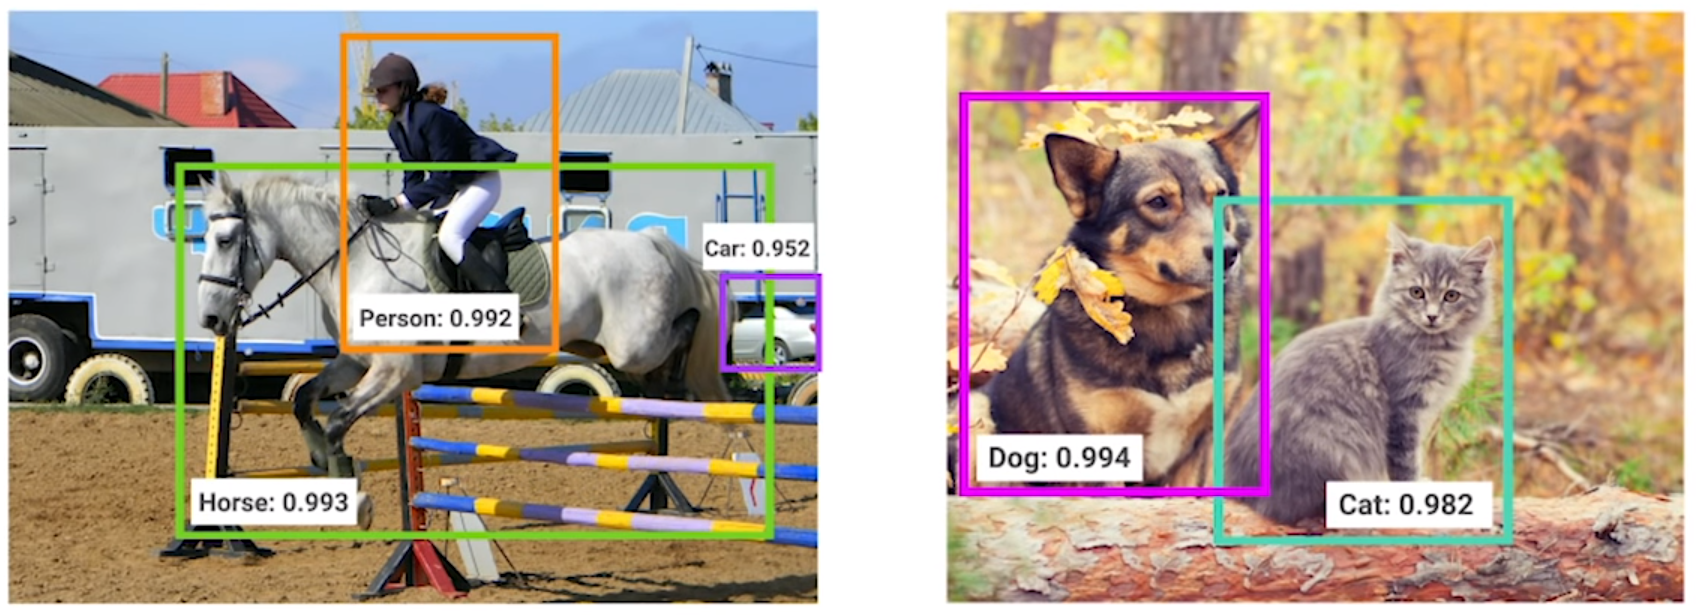
\includegraphics[scale=0.3]{figures/googleImages-ex-labeling.png}
  \caption{Example of Google Images' photo's labelling. Figure extracted from \cite{Google-2}}
  \label{fig:googleImages-ex-labelling}
\end{figure}


\newpage
\subsection{Face recognition}
As you can imagine, no face can exactly be the same as another face. Every face has different features specific to each which can be the size of your mouth, the distance between your eyes or even the form of your face. This is how image classification is used in face recognition technology. These features are extracted and analysed to recognize and evaluate which face belongs to which person. As said, every face has different specific features which are characterized by \textbf{keypoints} which are essential to mark and extract. An example of keypoints extraction is given in \autoref{fig:face-recognition-keypoints}. The most used technique to extract these features is CNN which is, of course, not only used for facial recognition. 

Facial recognition is used recurrently in various fields, here are some examples of face recognition applications:  
\begin{itemize}
\item \textbf{Security and control}: face recognition systems help control access to personal devices, residences, vehicles, offices and other premises alike. It can also be used to secure online payments with face recognition confirmation. 
\item \textbf{Health}: some specific features of the face are an evidence of illnesses. These features could be detected with facial recognition. 
\item \textbf{Criminal identification}: as presented in detective movies, creating a photofit picture is a way to identify criminals to find him in the population database\footnote{Indeed, the FBI currently have a database which includes half of the national population's faces.} thanks to face recognition.    
\end{itemize}

% https://hackernoon.com/building-a-facial-recognition-pipeline-with-deep-learning-in-tensorflow-66e7645015b8
\begin{figure}[h]
  \centering
  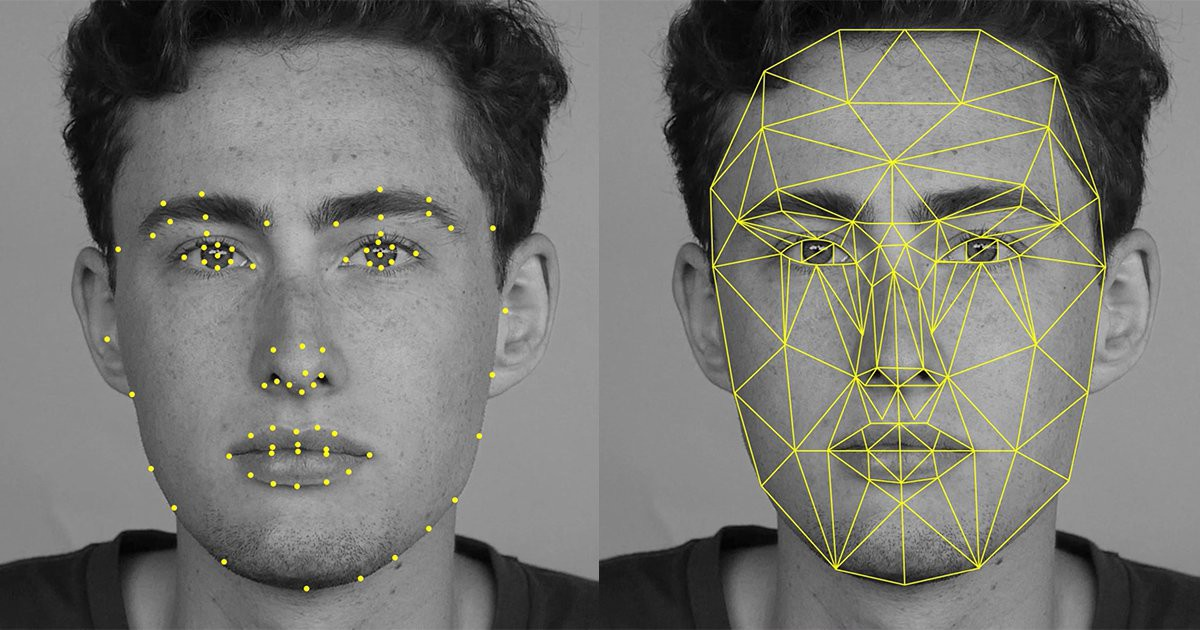
\includegraphics[scale=0.20]{figures/face-recognition-keypoints.jpeg}
  \caption{Keypoints marking to extract features for face recognition. Figure extracted from \cite{Face-Recognition-1}}
  \label{fig:face-recognition-keypoints}
\end{figure}

\subsection{Musical images analysis}
Actually, music is easily represented by images. It can be in the form of music score or spectral density, every song has its proper visual representation. Image recognition technology can be used to recognize the song obviously, but also to classify a large dataset of songs by genre. What was said about the presence of images in our daily life is also valid for music. Indeed, the music's market is growing and new genres are created over the multiple genres already existing. Applications that allows you to listen music (such as Spotify or Deezer) have to classify all their music library by genre. This is especially useful for the songs recommendations that the software is proposing to you following your music preferences or simply to find a specific song in the large library. \\ 

% source : https://pdfs.semanticscholar.org/22bf/c923870688d47fe3e4e97c52ab119a028f27.pdf
Concerning image processing, the overall procedure is the same as for simple images. the genre classification process of music has two main steps: feature extraction and classification. The first step obtains audio signal information, while the second one classifies the music into various genres according to extracted features. For instance, for music score analysis, one of the interesting features are the notes and their rhythm so that we have to create a model that recognizing musical notation as illustrated in \autoref{fig:partition-example}. To do that, it exists different methods that will be tackled further in the document such as CNN or Markov models. 

\begin{figure}[h]
  \centering
  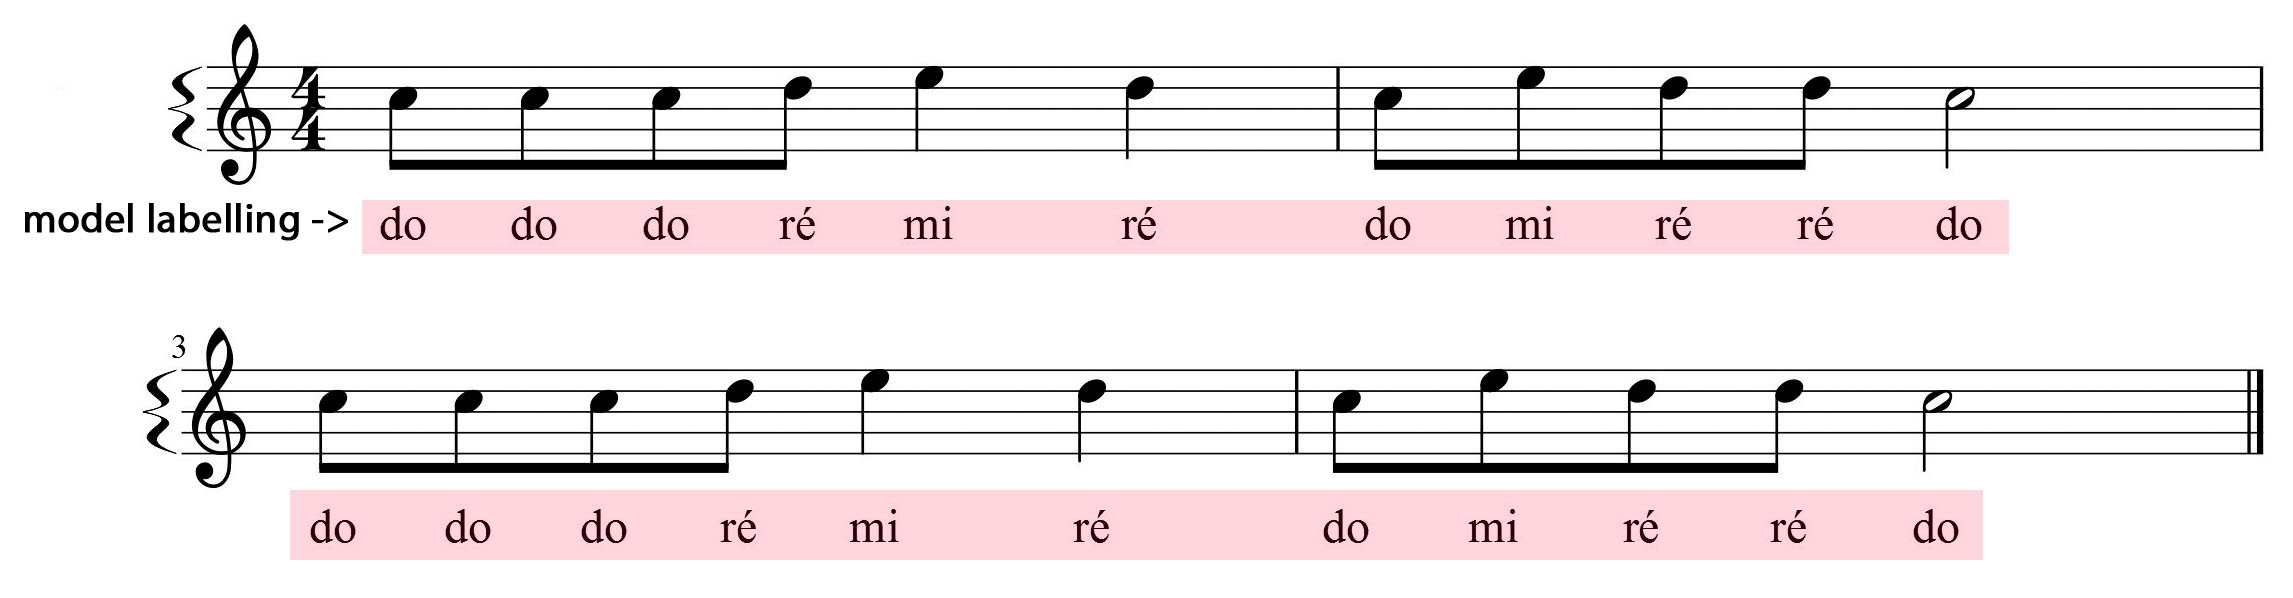
\includegraphics[scale=0.18]{figures/partition-example.jpg}
  \caption{(French) Labelling of the different notes of "Au clair de la lune" 's music score}
  \label{fig:partition-example}
\end{figure}
  
More generally, what is applied to music can also be applied to recognize sounds in general such as dog's bark, riding moto or human voice in particular thanks to their spectrogram representation. The following figure is using Deep belief network (DBL), a class of neural network, to recognize the audio.

\begin{figure}[h]
  \centering
  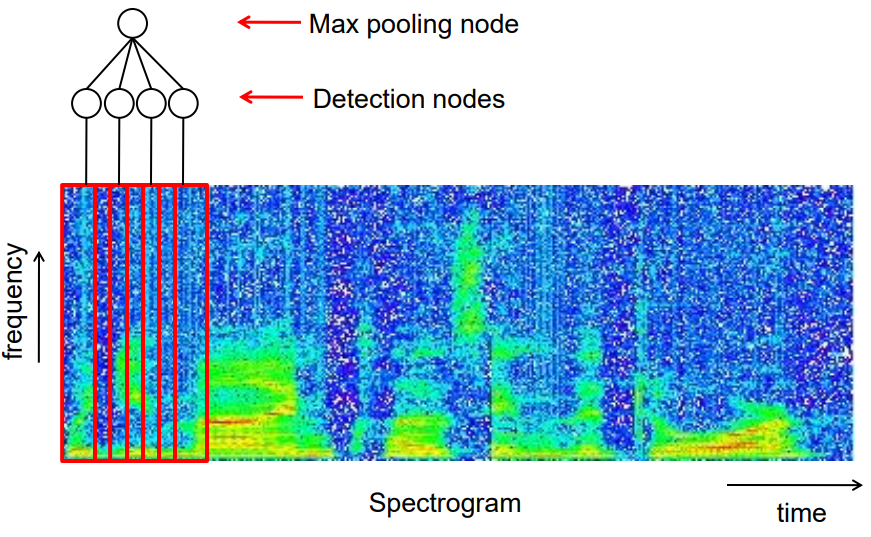
\includegraphics[scale=0.4]{figures/spectrogramSound.png}
  \caption{A sound spectrogram recognition using convolutional DBN. Figure extracted from \cite{sound}.}
  \label{fig:spectrogramSound}
\end{figure}


\subsection{Medical images analysis}
% Faire une grosse paranthèse sur le domaine médical % faire un lien avec facial recognition, on peut voir les diseases en fonction du visage
In the medical field, different techniques of medical images exist which make the use of images quite abundant. The most popular one are radiography or ultrasounds scan, but much more imaging techniques exist such as magnetic resonance imaging (MRI) or histological images observed under a microscope. This huge amount of images generated is a precious source of information and constitutes an important training dataset to help to extract important and redundant features for future analysis. Thus, the existing methods for image classification can also used for medical image analysis. The main goal of these methods is to highlight anomalies that may help to detect diseases. Deep learning excels in perceptual tasks such as detection and segmentation. Here are some examples of different types of medical images analysis and their reason for being used.

\begin{enumerate}
\item \textbf{mammographic mass classification:} this is actually one of the most frequent disease for women over a certain age. The important thing is to detect the disease at starting point to treat it correctly. Thus, what we want to detect here is a center of a lesion, especially to detect malignant tumor which is a sign of breast cancer.  To do that, the image includes different types of features that are used to raise the lesion such as contrast features that highlight a feature that is often mentioned by radiologists which is the distance that separates the lesion from the background. An other feature that is relevant to raise is the presence of holes in the candidate lesion which often decrease their suspiciousness, since tumours are solid, with possibly the exception of lobular carcinoma\footnote{From the \textit{National Cancer Institute} (NCI) \cite{NCI}: Cancer that begins in the lobules (milk glands) of the breast. Lobular carcinoma is a noninvasive condition in which abnormal cells are found in the lobules of the breast. Lobular carcinoma rarely becomes invasive cancer, but having lobular carcinoma in one breast increases the risk of developing invasive cancer in either breast.} \cite{breast-cancer-2}. This is just two types of features that is relevant to analyse mammographic mass but they are many more.  In particular, breast cancer detection is subject of an entire part of the document (\autoref{chap:breast-cancer}).

\begin{figure}[h]
  \centering
  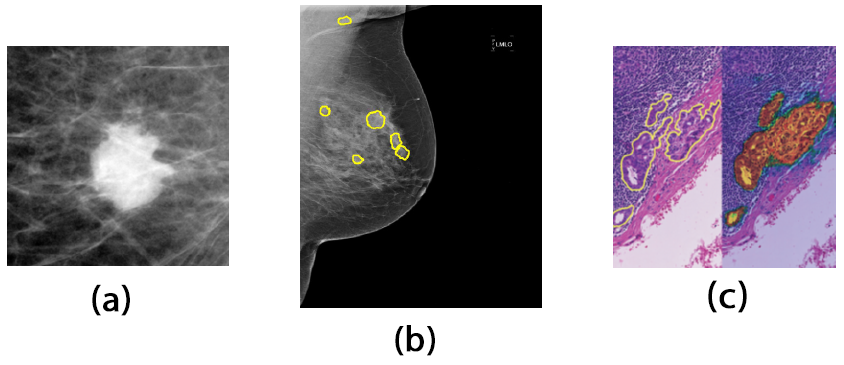
\includegraphics[scale=0.4]{figures/breast-images-examples.png}
  \caption{Mammographic mass images classification. (a, b) Segmentation of lesion, (a) is the illustration of the lesion on a smaller scale. (c) breast cancer metastases detection in lymph nodes using an histopathology image. Figures extracted from \cite{breast-cancer-2}}
  \label{fig:breast-example}
\end{figure}

\item \textbf{segmentation of lesions in the brain:} brain tumors can easily lead to death if they are not detected early and accurately to avoid disasters. Thus, brain tumors segmentation is an important challenge for medical purposes. Magnetic Resonance Imaging (MRI) is the medical imaging technique which is extensively used for diagnosis and treatment of brain tumors in clinical practice. Of course, these images provided by MRI includes different patterns of tumors which are interesting to collect to detect it automatically from deep learning and AI techniques. \\
Usually, healthy brain tissue consists of three parts: gray matter, white matter, and cerebrospinal fluid. The segmentation is used to identify areas surrounded by a tumor by separating the active tumorous tissue from the necrotic tissue. This is done by identifying abnormal areas when compared to normal tissue \cite{brain-tumor-1}. 

\begin{figure}[h]
  \centering
  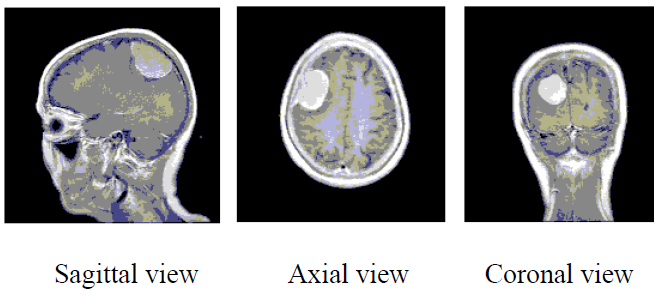
\includegraphics[scale=0.5]{figures/brain-images-examples.png}
  \caption{Brain MRI slices captured from different directions. Figure extracted from \cite{brain-tumor-1}.}
  \label{fig:brain-example}
\end{figure}

\newpage
\item \textbf{diabetic retinopathy (DR) classification :} DR is an eye deficiency created by diabetes and can lead to blindness. The main purposes of this deficiency is due to the high-level of sugar in your blood which can lead to the blockage of the tiny blood vessels that nourish the retina, cutting off its blood supply. Classification methods and pattern recognition are tried to help analysing color fundus photographies (which is represented in the figure) to detect DR automatically and are actually in good progress. These classifying models are capable of quantifying the different features as blood vessels, fluid drip, exudates, hemorrhages and micro aneurysms\footnote{A micro aneurysm is a small swelling that forms in the wall of tiny blood vessels. These small swellings may break and allow blood to leak into nearby tissue.} into different classes. All these features are signs of DR, especially micro aneurysms which is usually the first visible sign of diabetic retinopathy. \\
Many filters are used to highlight these features such as edges detection which is the one of the feature extraction methods where the boundaries of the features are highlighted (i.e., the edges of the blood clots, white lesions, veins) are detected based on the sudden change in the pixel values with the neighborhood pixel intensity \cite{DR-1}.

\begin{figure}[h]
  \centering
  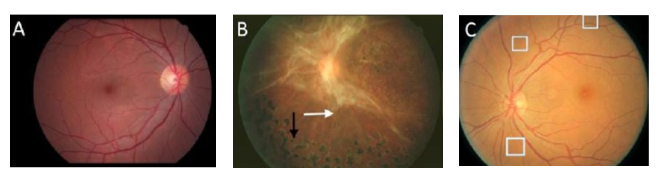
\includegraphics[scale=0.6]{figures/DR-images-examples.png}
  \caption{Representative retinal images of DR at various stages of the disease, as labeled: A- normal, B- end stage, C- early stage. Arrows in B point to pathological indications. White boxes in C enclose very small lesions that the CNNs have difficulty discerning. Figure extracted from \cite{DR-2}.}
  \label{fig:DR-example}
\end{figure}

\end{enumerate}

However, the outcomes of these methods of image processing is not sufficient to give complete information about the image. The computer has not yet the knowledge of scientists and doctors which means that a human's intervention is necessary to complete the information given by the computer's outcomes. That is why the deep learning methods used are rather called \textbf{computer aided detection} (CAD) which is defined as systems that assist doctors in the interpretation of medical images. 

\chapter{General concepts of AI}

\section{Machine learning and deep learning}
We know that image classification is a problem resolvable by AI methods such as machine learning and especially deep learning. These methods are usually used to resolve data science problems such as image classification. Let's introduce and define them.

\subsection{Machine learning}

\begin{defn}
\textit{Machine learning} is an application of artificial intelligence (AI) that provides systems the ability to automatically learn and improve from experience without being explicitly programmed. Machine learning focuses on the development of computer programs that can access data and use it learn for themselves \cite{ML-1}. 
\end{defn}

% source : https://searchenterpriseai.techtarget.com/definition/machine-learning-ML
The main goal of machine learning is then to allow the computers \textbf{learn automatically} without human intervention to find a model that does an approximation of reality by doing predictions. Nevertheless, there exists different types of learning whose supervised and unsupervised learning -- which are defined thereafter, where in the first case, data are pretreated by humans while in the second case it does not need it and use instead an iterative approach to review data and arrive at conclusions which is object of deep learning. 

\subsubsection{Supervised and unsupervised learning} \label{sec:supervised-unsupervised}

\begin{defn}
\textit{Supervised} learning is a type of system in which both input and desired output data are provided. Input and output data are labelled for classification to provide a learning basis for future data processing \cite{Supervised-1}. 
\end{defn}

\begin{exmp}
A simple example for \textit{supervised} learning. Given the dataset presented in \autoref{table:ex1-supervised}, the machine can easily compute the output $y$ of input $x$. 
If $x = 10$, the computer will output $y = 100$ by learning the pattern of squaring the input thanks to the provided dataset.  

\newpage
\begin{center}
    \begin{tabular}{|c|c|}
      \hline
      Input $x$ & Output $y$ \\
      \hline
      1 & 1 \\
      \hline
      2 & 4 \\
      \hline
      3 & 9 \\
      \hline
      4 & 16 \\
      \hline
    \end{tabular}
    \captionof{table}{Example of dataset for supervised learning}
    \label{table:ex1-supervised}
\end{center}
\end{exmp}

Note that in supervised learning, machine learning cannot be used without a good dataset. Before using machine learning to models and evaluates new data, we need to give him a relevant and useful set of data to allow him to learn correctly. If what we are interested for is a specific feature, the data should be adapted to highlight and label this specific feature to ease the learning of the machine. Once data are correctly pretreated, the machine will use this dataset called \textbf{training set} to learn from it and acquire knowledge about the data to apply it to new data.

\begin{figure}[h]
  \centering
  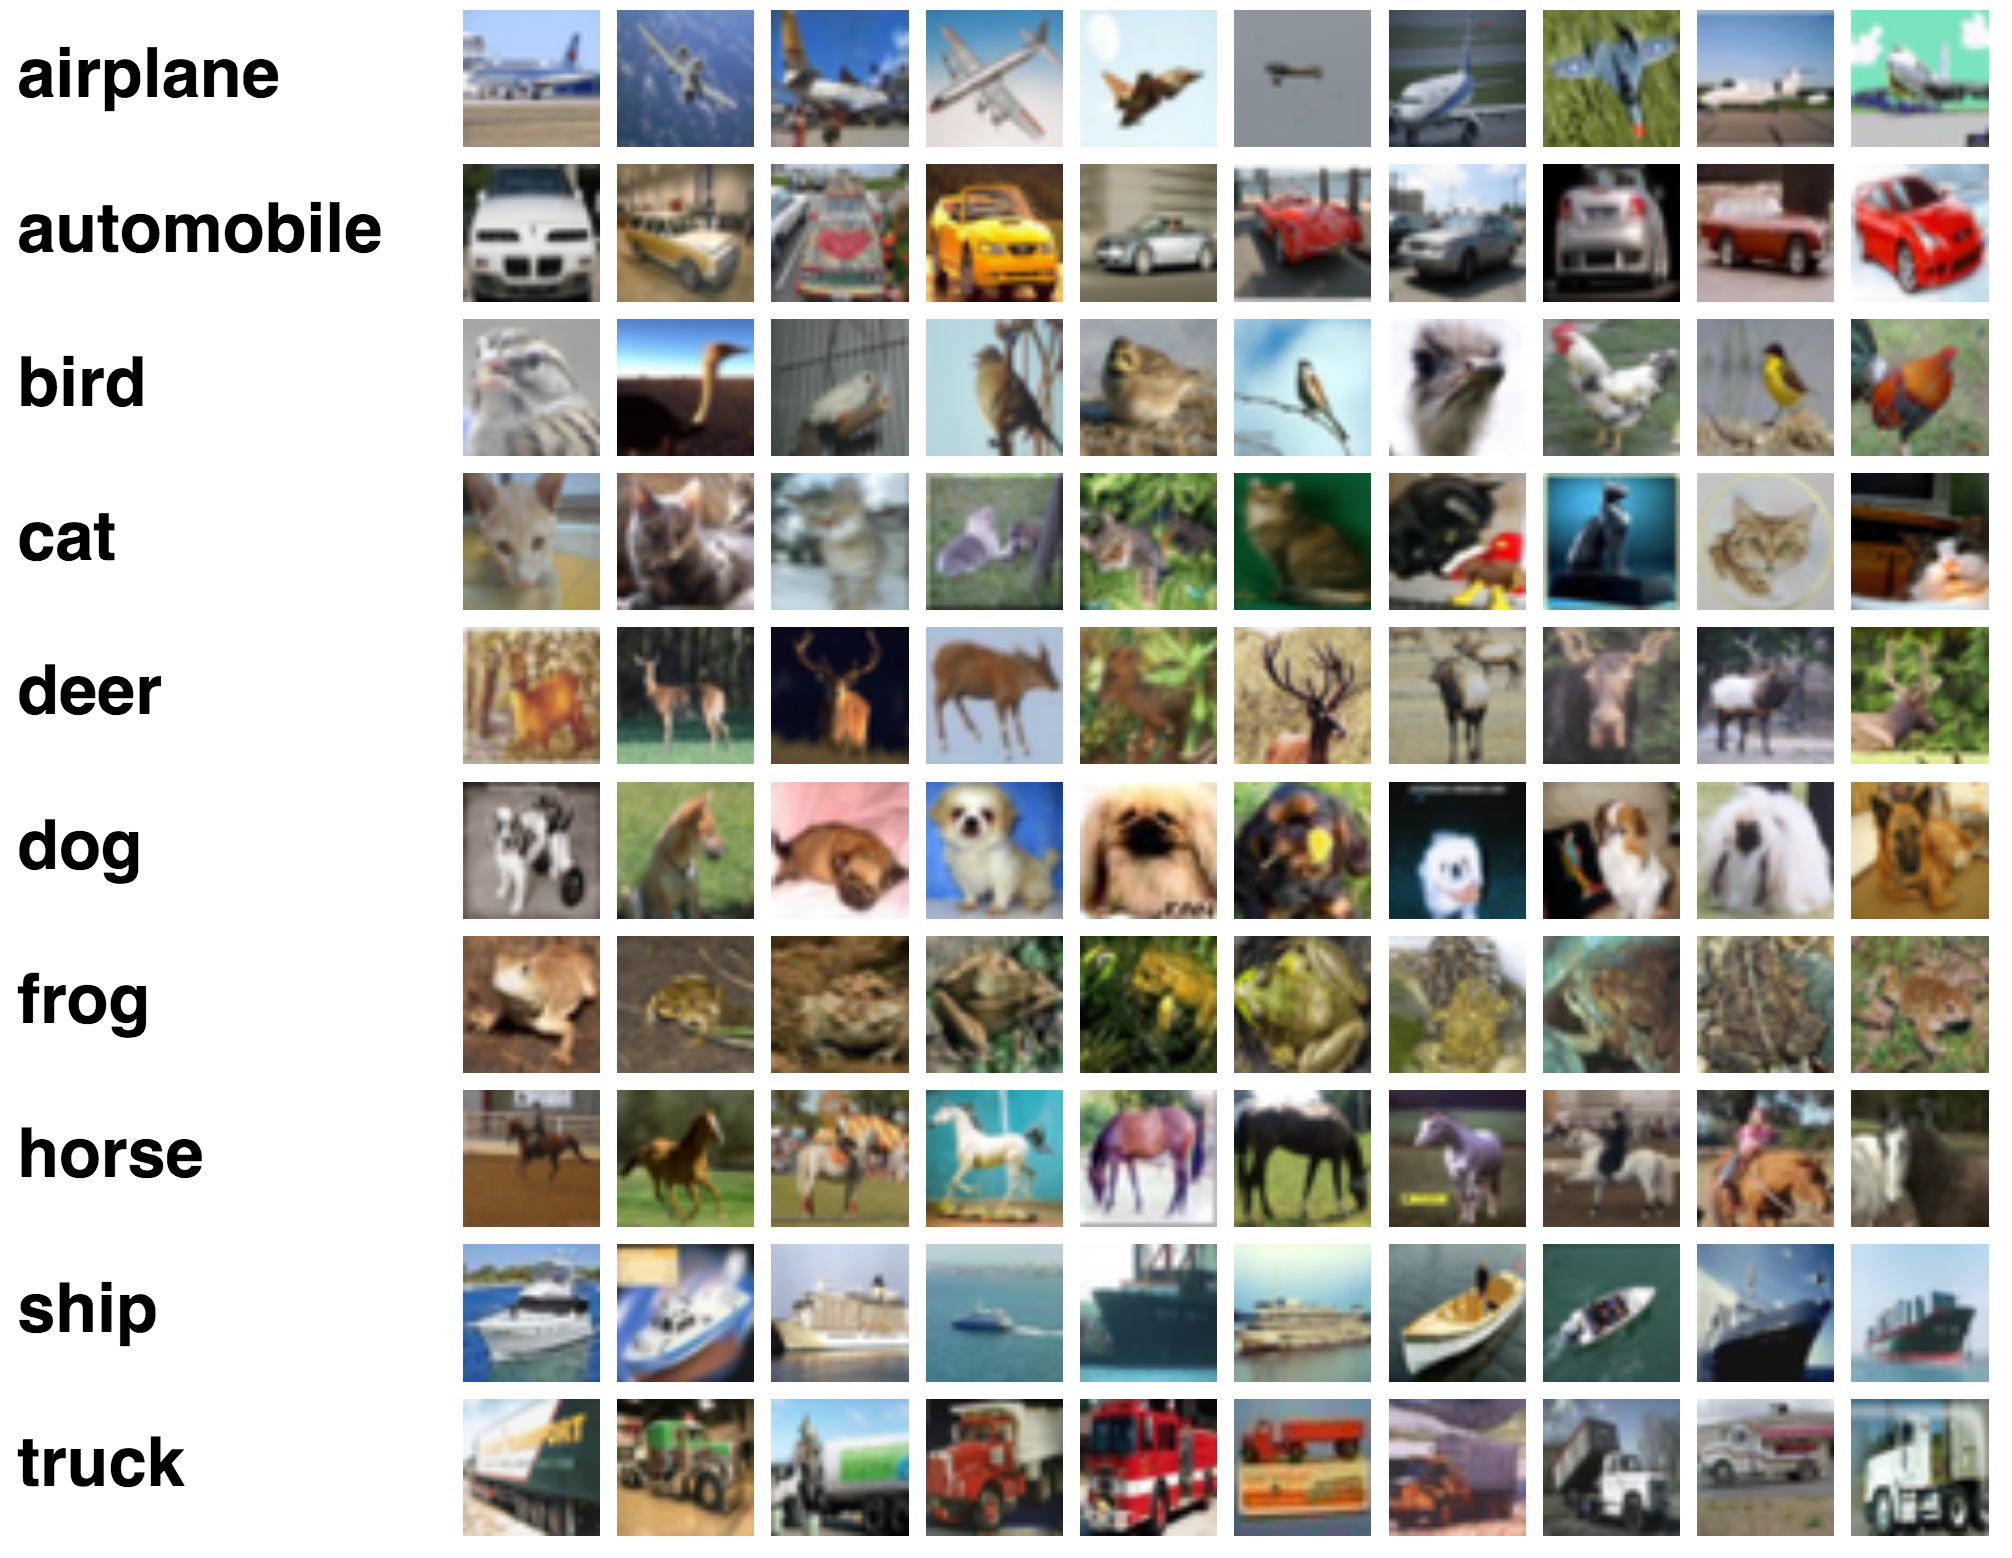
\includegraphics[scale=0.25]{figures/cifar10.png}
  \caption{Example of training dataset : CIFAR-10. Figure extracted from \cite{CIFAR10}.}
  \label{fig:cifar10}
\end{figure}

\begin{defn}
\textit{Unsupervised} learning is the training of an AI algorithm using information that is neither classified nor labeled and allowing the algorithm to act on that information without guidance, i.e. data are unlabeled and the system’s algorithms act on the data without prior training \cite{Unsupervised-1}. 
\end{defn}

\begin{exmp}
Compared to supervised learning, in unsupervised learning \textbf{only inputs} are given as dataset which means that there is no output to match to. As simple example, given a group of people, we are trying separate them in different categories. The machine has different ways to classify them: their ethnicity, their hair colors, their gender, etc. But no one is giving information to the machine about the right way to divide the group. The machine has to learn without any supervisor. That is what unsupervised learning means.   To resolve this, different methods of \textit{clustering} algorithms exist and will be used to run through the data and find natural clusters if they exist. % on va en parler plus tard des =/= méthodes des clustering, lien utile pour plus tard: https://blog.algorithmia.com/introduction-to-unsupervised-learning/

\end{exmp}    

% https://towardsdatascience.com/deep-learning-for-image-classification-why-its-challenging-where-we-ve-been-and-what-s-next-93b56948fcef
\begin{figure}[h]
  \centering
  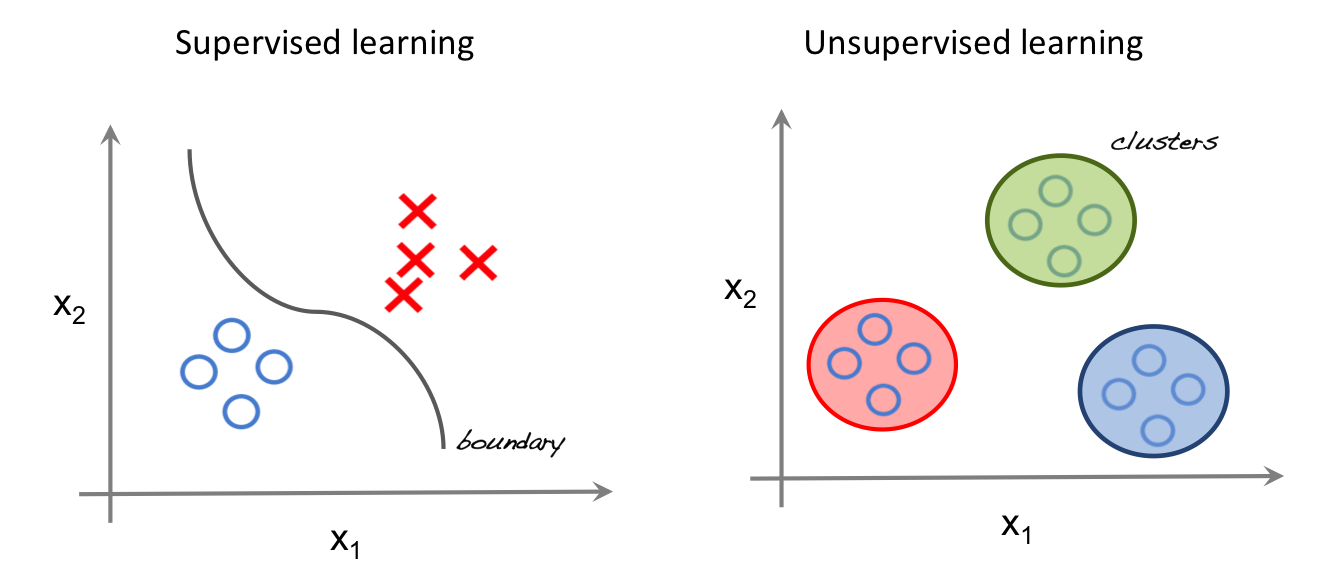
\includegraphics[scale=0.32]{figures/supervised-unsupervised.png}
  \caption{Supervised learning VS Unsupervised learning. In supervised learning, the separation and the categories are well defined while in unsupervised learning, clusters have to be found. Figure extracted from \cite{supervisedVSunsupervised-1}}
  \label{fig:supervised-unsupervised}
\end{figure}


\newpage
\subsubsection{Categories of machine learning} \label{sec:categories-ML}
% https://openclassrooms.com/fr/courses/4011851-initiez-vous-au-machine-learning/4120981-comment-se-passe-lapprentissage-dun-modele
% https://towardsdatascience.com/machine-learning-general-process-8f1b510bd8af
% linear regression, logistic regression, decision trees, support vector machines, and neural networks, as well as non-parametric models such as k-Nearest Neighbors.
Machine learning is divided into 4 main categories which are classification, regression, clustering and dimensionality reduction. The two first are generally used for supervised learning while clustering is more often used for unsupervised learning. Regarding dimensionality reduction, its function is to transform data to highly dimensional data which could be used for both types of learning. Let's now introduce and define these terms. 

\begin{defn}
\textit{Classification} algorithms are used when the desired output is a discrete label. In other words, they're helpful when the answer to your question about your business falls under a finite set of possible outcomes \cite{class-regression-1}. 
When the set of possible outcomes is composed by only two elements, such as returning if an image has been forged or not, is called binary classification. 
\end{defn}

\begin{defn}
\textit{Regression} is useful for predicting outputs that are continuous. That means the answer to the question is represented by a quantity that can be flexibly determined based on the inputs of the model rather than being confined to a set of possible labels \cite{class-regression-1}. We are trying to map input variables to some continuous functions. 
\end{defn}

\begin{defn}
\textit{Clustering} is the assignment of objects to homogeneous groups (called clusters) while making sure that objects in different groups are not similar. As said, clustering is considered an unsupervised task as it aims to describe the hidden structure (features) of the objects \cite{clustering-dimensionalityReduction-1}  . 
\end{defn}

\begin{defn}
As its name said, \textit{dimensionality reduction} is a process where its main objective is to reduce the number of random variables under consideration to treat smaller and specific data. The number of features under consideration decreases, where each feature is a dimension that partly represents the objects.
\end{defn}

\begin{figure}[h]
  \centering
  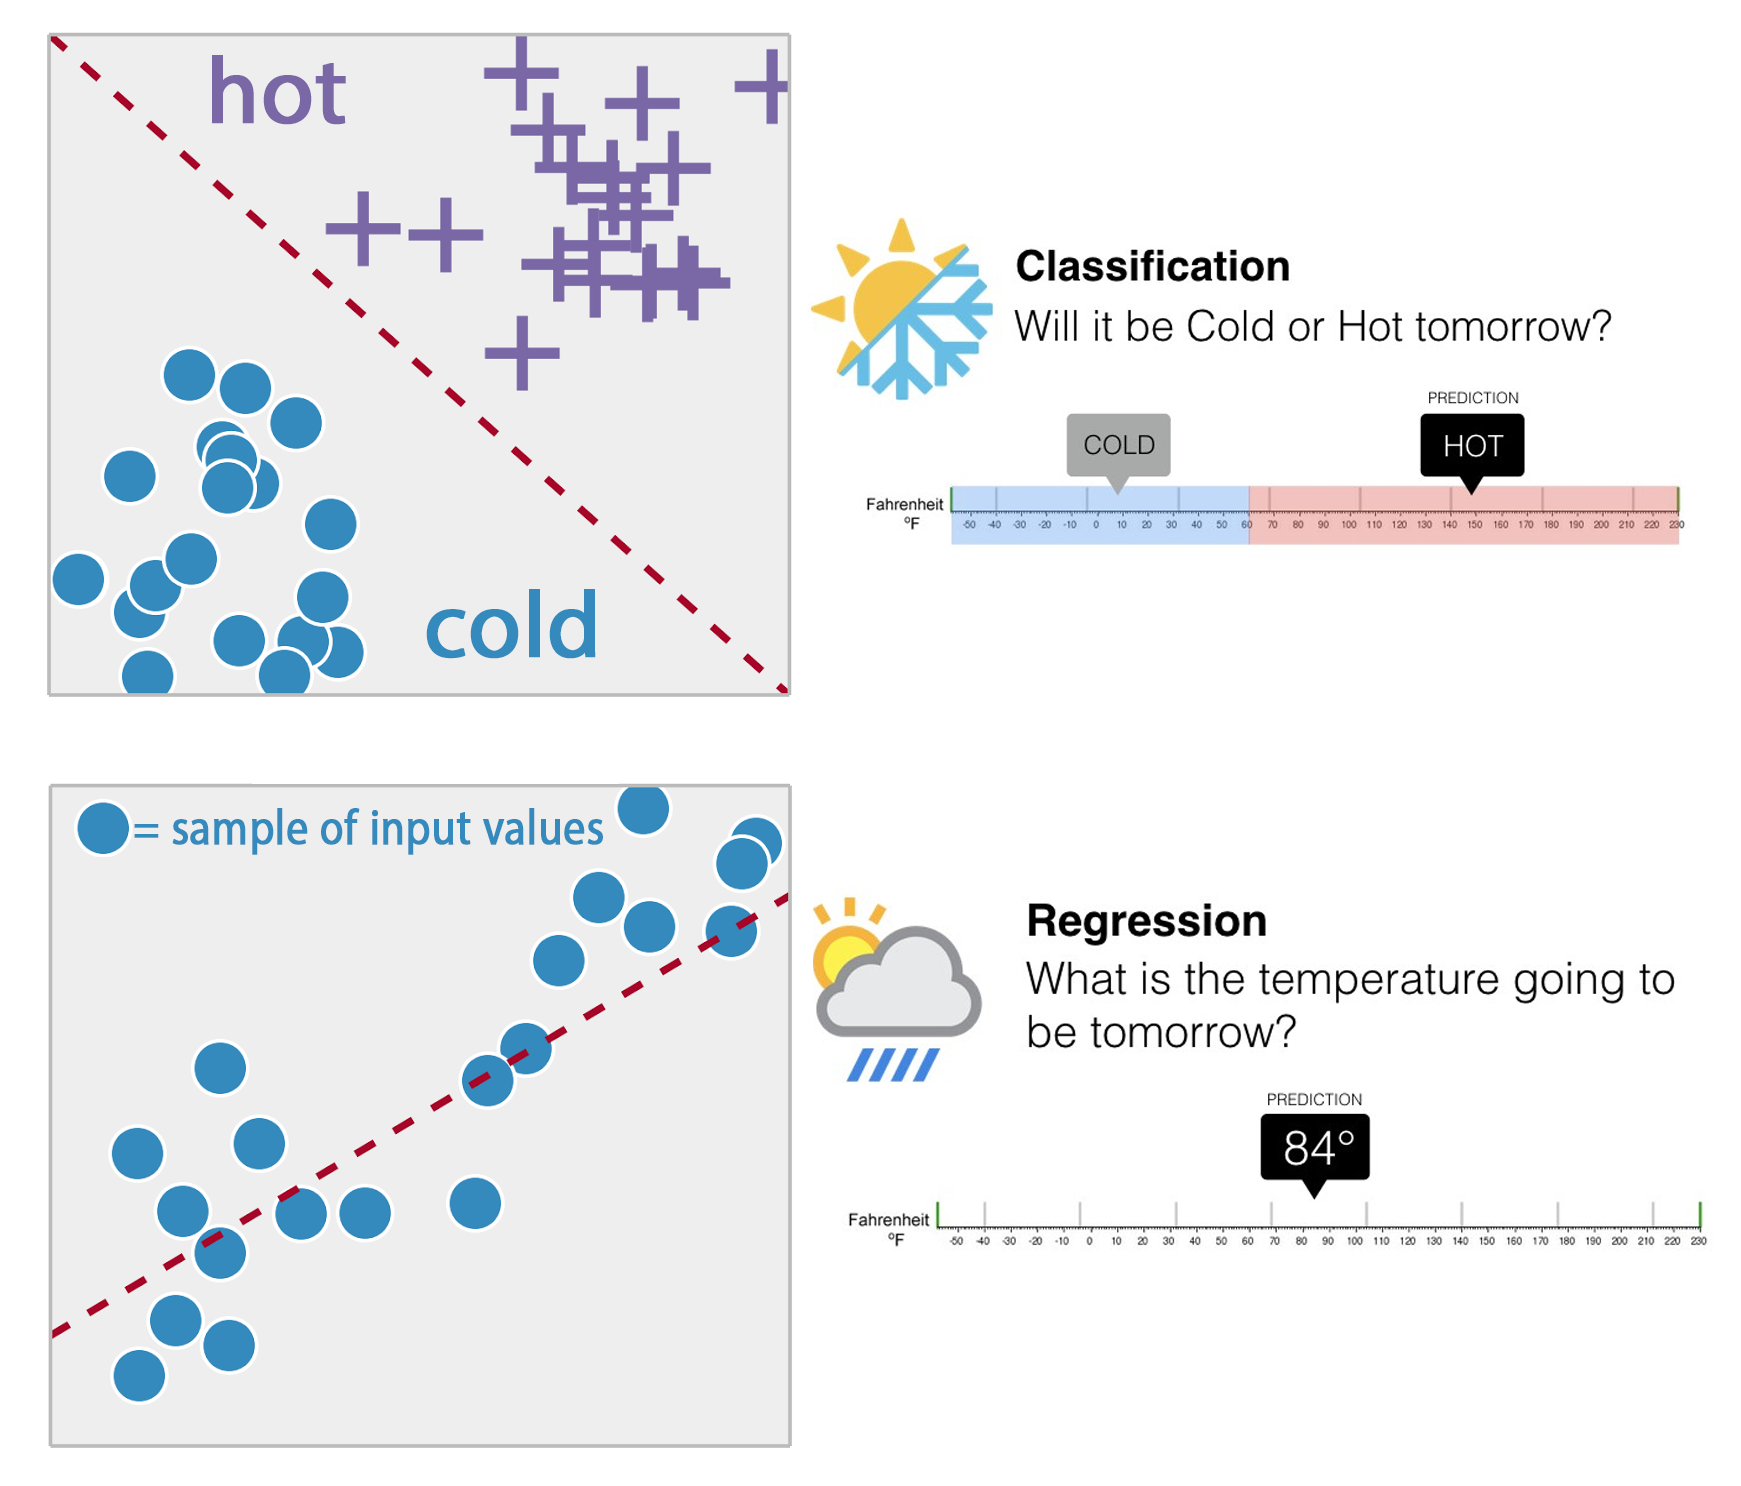
\includegraphics[scale=0.8]{figures/classification-regression.png}
  \caption{Difference between classification and regression on a weather example. For classification, we are doing a clear separation between two classes : hot and cold. For regression, we are trying to mean the degrees values given on input by a certain function. Figure adapted from \cite{fig_class_regression}}
  \label{fig:classification-regression}
\end{figure}

\newpage
\subsection{Deep learning}

\begin{defn}
\textit{Deep learning} is an artificial intelligence function that imitates the workings of the human brain in processing data and creating patterns for use in decision making. Deep learning is a subset of machine learning in artificial intelligence (AI) that has networks capable of learning unsupervised from data that is unstructured or unlabeled. Also known as deep neural learning or deep neural network \cite{DL-1}. 
\end{defn}

Contrary to simple machine learning, deep learning is thus used to treat data that do not need to be pretreated and then used for unsupervised learning. To do that, deep learning will use artificial neural networks inspired by human's brain. This network is composed by a certain number of layers (which explains the term "deep" in "deep learning") where every layer receives and interprets informations of previous layer. To see more details, neural networks make object of \autoref{sec:neural-networks}.  

\subsubsection{Differences between machine learning and deep learning}
Of course, machine learning and deep learning are both used. Some difference make machine learning more useful than deep learning in a specific case and vice versa. Some of those difference are presented below: 
\begin{itemize}
\item Machine learning (ML) uses statistical learning algorithms to treat labelled data while deep learning (DL) uses neural networks to treat unlabelled data.
\item On one hand (ML), raw data are labelled manually by a data scientist to give a "clean" dataset to the machine. On the other hand (DL) , raw data are directly given to the machine which will uses its neurons to extract features. 
\item ML uses linear learning techniques while DL uses a non-linear architecture which its complexity is growing proportionally to the number of neurons.   
\item ... in summary, ML has a \textbf{supervisor} (human) to learn while DL does not have. 
\item But both ML and DL are able to handle massive dataset sizes, however, ML methods make much more sense with small datasets. 
\end{itemize} 
 
\begin{figure}[h]
  \centering
  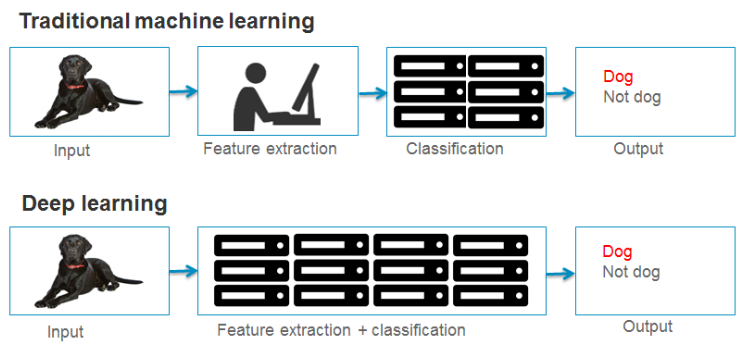
\includegraphics[scale=0.65]{figures/machineVSdeep.png}
  \caption{Illustration of the main difference between machine learning and deep learning}
  \label{fig:machineVSdeep}
\end{figure}


\section{Definition of image classification problem}
% lien utile : https://developers.google.com/machine-learning/practica/image-classification/ 
Recognize an animal from an object is a trivial task for humans but how about machines? A machine cannot assert with a 100\% accuracy if an image contains such or such thing. That proves that classify images seems to be a complex task for machines. Thus, the main objective of image classification problem is to converge towards a perfect accuracy. 

Basically, \textbf{image classification is the task of categorizing images into different classes}. This problem can be extended into other computer vision problems, such as localization, detection, and segmentation. However, it can either be a supervised learning problem or an unsupervised learning problem. 

\begin{defn}
\textit{Supervised image classification} is a problem where we have to define a set of target classes (for instance, objects to identify in images), and train a model to recognize them using labelled example photos \cite{Google-2}. The idea is that a user can select sample pixels in an image that are representative of specific classes and then softwares apply it on new images to retrieve features of these specific classes used as reference. 
\end{defn}

\begin{defn}
\textit{Unsupervised image classification} is a problem where the outcomes (clusters of pixels with same features) are based on the software analysis of an image without the user providing sample classes. The computer uses techniques to determine which pixels are related and groups them into classes. 
\end{defn}

\begin{figure}[h]
  \centering
  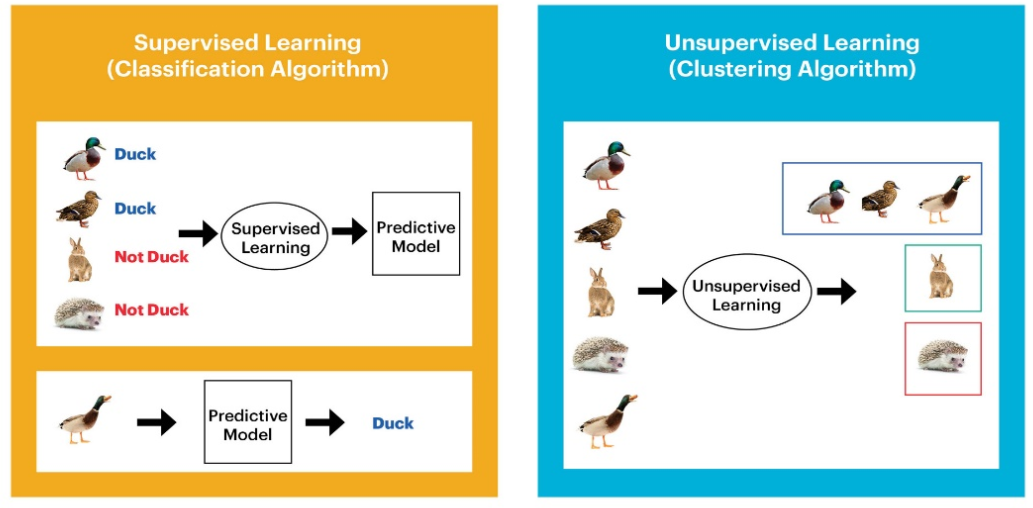
\includegraphics[scale=0.5]{figures/supervised-unsupervised-2.png}
  \caption{Supervised classification VS Unsupervised classification. Figure extracted from \cite{supervisedVSunsupervised-2}}
  \label{fig:supervised-unsupervised-2}
\end{figure}

\subsection{Which methods should we use?}
% présenter les différents cas quand on utilise supervisé, pareil pour non supervisés et présneter les avantages de l'un par rapport à l'autre
% https://www.mathworks.com/discovery/machine-learning.html
It exists different methods whether for supervised or unsupervised learning and all of them are useful. There exists no method better than an other one. Choosing the method depends of different criteria whose information missed, size of data, the insights you want to get from the data, etc. Generally, supervised learning is used to train a model to \textbf{make a prediction}. It can be used for instance for weather forecast and more generally for continuous and linear variables. On the other hand, unsupervised learning is employed to explore data and train a model to \textbf{find clusters} into the data. Some of the most familiar methods are \textit{Support Vector Machine} (SVM), nearest neighbour, maximum likelihood, decision tree classifier for supervised learning. Concerning unsupervised learning, K-means clustering algorithm or neural networks are the most common methods. 
% All these methods will be tackled later.. 




\chapter{Materials and Methods} % etat de l'art
% Cas particulier -> reconnaissance d'image facile comme les lettres  
% https://arxiv.org/pdf/1705.02680.pdf
% example lettres : https://www.youtube.com/watch?v=mmXB636p_E8
% Cas particulier (domaine médical) -> à définir 
% cancer du sein : https://peerj.com/articles/6201.pdf 

%\textit{\textbf{Plan du chapitre:} état de l'art - présentation des méthodes utilisés dans les références traités ainsi que des résultats (comparaison). Focus sur le cas du cancer du sein selon l'article : "Breast cancer detection using deep convolutional neural networks and support vector machines". Les deux premières sections introduisent CNN et SVM : les deux méthodes de classification principales utilisés dans l'article. S'en suit la méthodologie complète présentée dans l'article ainsi que les résultats obtenus.} 

In this chapter, different methods of learning are introduce and presented. In particular, neural networks is the main and most known method for images classification especially convolutional neural networks (CNN). In a second time, support vector machines (SVM) models are presented to associate learning algorithms that analyse data used for classification and regression analysis. Finally, we take interested of the evaluation methods: how do we evaluate the classification? From which percentage is the evaluation correct? Therefore, this evaluation leads to a question of validation to define how do we validate a prediction.


\section{Neural networks} \label{sec:neural-networks}
% parler de ANN -> pourquoi c'est pas suffisant et pourquoi on a besoin de CNN ? 
% https://uv.ulb.ac.be/pluginfile.php/1393702/mod_resource/content/1/NeuralNetworks.pdf
% http://www.cs.tau.ac.il/~dcor/Graphics/pdf.slides/YY-Deep%20Learning.pdf 
% définition / intro à CNN 
% parler vite fait de ANN etc mais SURTOUT bien parler de CNN car c'est ce qui est utilisé dans la classification d'images pour détecter les patterns
When speaking about deep learning, the most known technique is probably neural networks. Formally, the simplest definition of a neural network, more properly referred to as an 'artificial' neural network (ANN), is provided by the inventor of one of the first neurocomputers, Dr. Robert Hecht-Nielsen:  

\begin{quote}
\textit{"A neural network is a computing system made up of a number of simple, highly interconnected processing elements, which process information by their dynamic state response to external inputs."}
\end{quote}    

% https://www.researchgate.net/publication/262936797_ARTIFICIAL_NEURAL_NETWORK_PART_1
This definition is somehow explaining how a human's brain work and this is mostly why a ANN is inspired of to recognize patterns. To imitate the behaviour of a human's brain, let's see first how does a brain works. Basically, the biological neural network is composed of four main elements:
somas, dendrites, axons and synapses. For a better understanding, we have to define their respective functions to create elements that will act similarly in our ANN.
\begin{itemize}
\item \textbf{Soma:} central part of a neuron, contains the cell nucleus which mainly contains all of the cell's genome (DNA). In ANN, this should correspond to the neurons. 
\item \textbf{Dendrite:} projection of a neuron that receive signals (information) from other neurons. In ANN, this should correspond to the inputs. 
\item \textbf{Axon:} carries nerve impulses away from the cell body. A neuron typically has one axon that connects it with other neurons or with muscle or gland cells. In ANN, this should correspond to the outputs. 
\item \textbf{Synapse:} transfer electric activity (information) from one cell to another.  In ANN, this should correspond to the links between every neuron and their respective weights which correspond to the strength or amplitude of a connection between two nodes. Besides, that's why this weight is also called \textit{synaptic weight}. 
\end{itemize} 

To sum up, we can associate these biological elements to artificial ones following \autoref{table:bio-ANN}. The representation of both neural networks are shown in \autoref{fig:bio-ANN}. 

\begin{center}
    \begin{tabular}{|c|c|}
      \hline
      Biological NN & Artificial NN \\
      \hline
      Soma & Neuron \\
      \hline
      Dendrite & Input \\
      \hline
      Axon & Output \\
      \hline
      Synapse & Weight \\
      \hline
    \end{tabular}
    \captionof{table}{Association of elements from biological neural network to articial neural network.}
    \label{table:bio-ANN}
\end{center}

\begin{figure}[h]
  \centering
  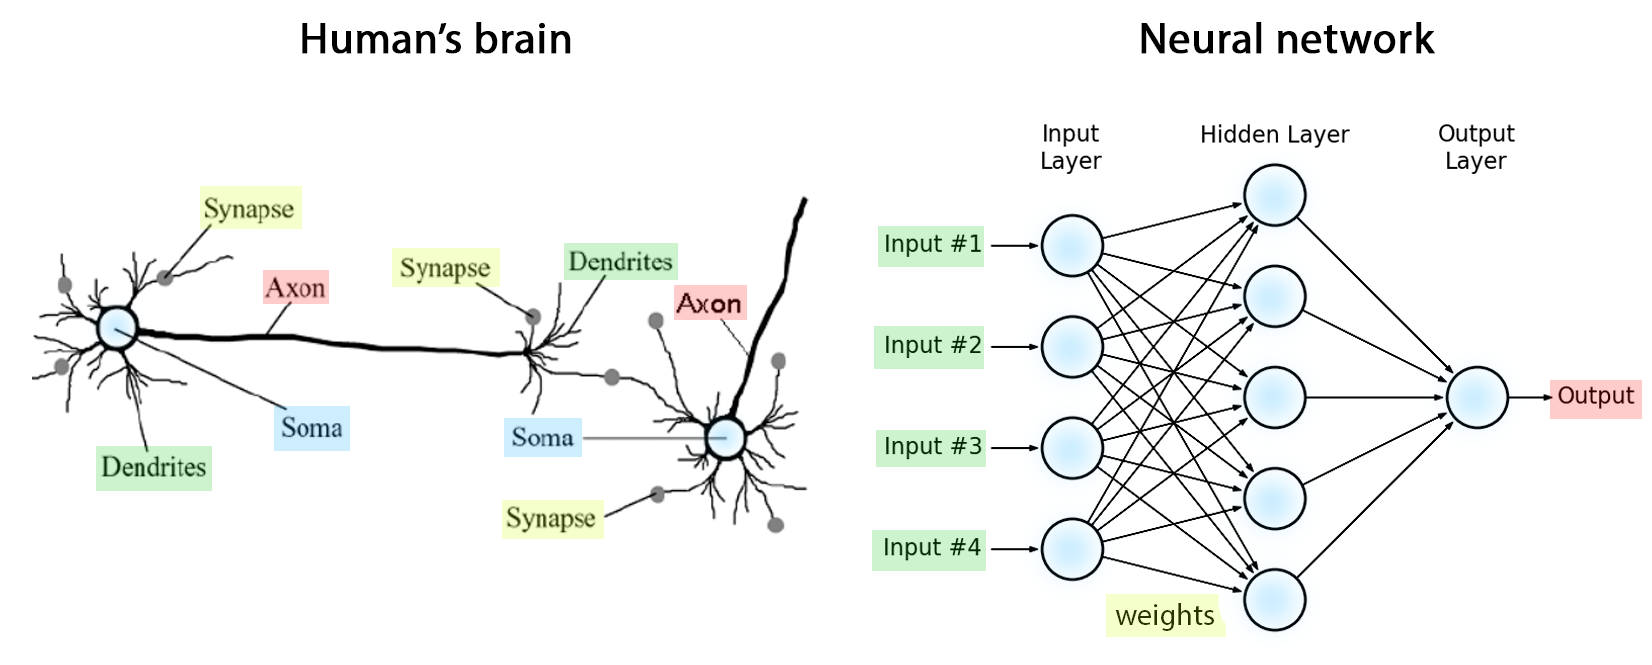
\includegraphics[scale=0.25]{figures/brainVSneuralnet.png}
  \caption{Comparison between a biological neural network and an ANN. The same color associates elements with the same function in a biological and artificial point of view.}
  \label{fig:bio-ANN}
\end{figure}

\subsection{How does neural network works?} \label{sec:nn-work}
Typically, a neural network is initially trained or fed large amounts of data. Training consists of providing input and telling the network what the output should be. The objective is to obtain a neural network that is trained and generalizes well that should behaves correctly on new instances of the learning task. To do that, we need an architecture of neural network composed by a set of neurons and links connecting neurons such that each link has a synaptic weight. Multiple neural network architectures exist such as single-layer or multi-layer perceptron. Inevitably, we need a learning algorithm to learn. Linear regression, logistic regression, decision tree or SVM are some examples of learning algorithms. The last one cited make object of \autoref{sec:svm}. 

Generally, a neural network is represented by the scheme presented below in \autoref{fig:nn-scheme}.

\begin{figure}[h]
  \centering
  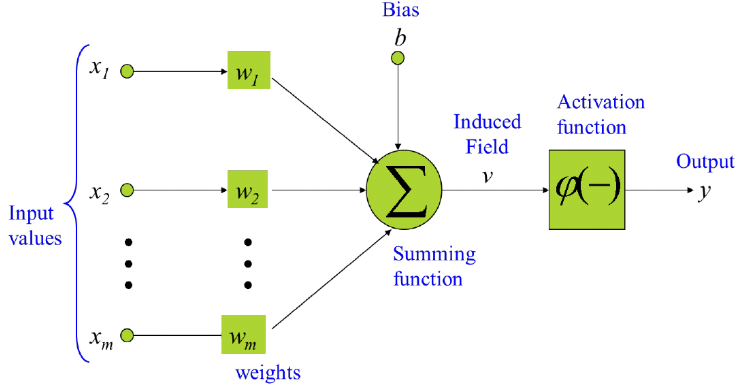
\includegraphics[scale=0.7]{figures/nn-scheme.png}
  \caption{General representation of a neural network. Figure extracted from \cite{neuralnet-course-1}.}
  \label{fig:nn-scheme}
\end{figure}

\newpage
Firstly, input values are given to the neural network. In the case of an image processing, the input will be given by each pixel of the image. For instance, if we try to process an image of 200x200 pixels, the input values will be defined by the set $\{x_{1}, x_{2}, ... , x_{39999}, x_{40000}\}$ where $x_{i}$ is a value that describes the level of a certain property (luminosity, contrast, ...) on the pixel. All these informations are given to \textbf{neurons}.

Neurons are functions consisting of a set of links described by synaptic weights which are computed by a summing (adder) function: 
$$ v_{j} = \sum_{i=1}^{n} x_{i} w_{ij} $$ where $n$ is the input number, $x_{i}$ the value of neuron $i$ and $w_{ij}$ the weight between neuron $i$ and neuron $j$. $v_{j}$ is called the local induced field of the neuron. 

Finally, this induced field added to a bias value $b$ are given to an activation function  $\phi$ (also called decision function) to determine the output value: 
$$ y = \phi(v + b)$$

Many types of activation function exist but in general, a sigmoid (and its derivative) is used for the statistical interpretation and is the most widely decision function used. The sigmoid is defined: 
$$ \phi(x) = \frac{1}{1+e^-x} $$ 
and its derivative:
$$ \phi'(x) = \phi(x)[1-\phi(x)] $$ 

The reason that sigmoid is one of the most used activation function is that it is a non-linear function which allow then to stack layers and to treat non-binary activations. Moreover, the output of the activation function is always going to be in range (0,1) compared to (-$\infty$, $\infty$) of linear function. Thus, an output with a value approaching 1 means that the prediction is most likely focused on this solution. 

\section{Convolutional neural networks} \label{sec:CNN}
Concerning image classification and recognition, traditional multilayer perceptron (MLP) models were a successfully method used. Nevertheless, due to the full connectivity between nodes they suffer from the curse of dimensionality, and thus do not scale well to higher resolution images. For example, a 1000×1000-pixel image with RGB color channels has 3 million weights, which is too high to feasibly process efficiently at scale with full connectivity \cite{wiki-cnn}. For this reason, scientists had to find an efficient solution to remedy this situation. That's why in the end of the 80's, convolutional neural network (CNN) were created. 

CNN is a type of neural network mostly applied for visual tasks such as image or video recognition.  A convolution is the simple application of a filter to an input that results in an activation. Thus, we are applying a filter of a fixed size $N \times N$ to every window of size $N \times N$ of the input image a number of times needed to filter the whole image. This filter is used to highlight the feature that we are interested in. CNN basically uses the same structure as a basic neural network: input, hidden and output layers. However, several difference occur especially for hidden layers. Indeed, the hidden layers of a CNN typically consist of convolutional layers, pooling layers and fully connected layers as shown in \autoref{fig:cnn-architecture} and detailed in the next sections. 

\begin{figure}[h]
  \centering
  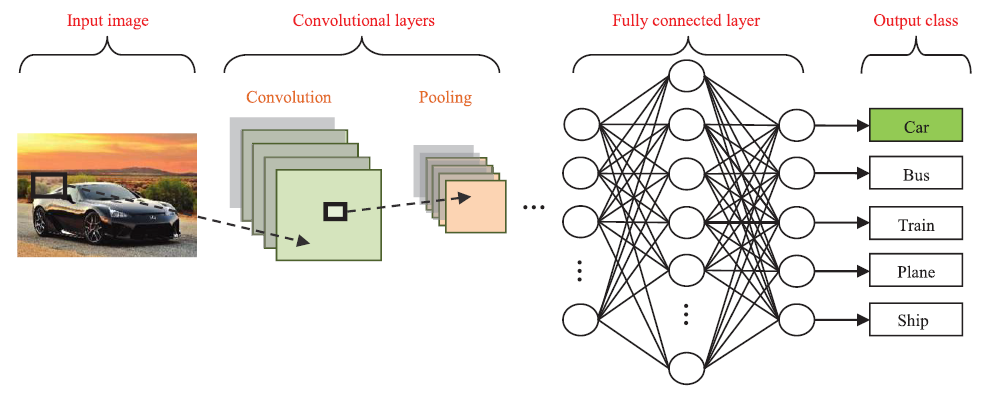
\includegraphics[scale=0.55]{figures/cnn-architecture.png}
  \caption{CNN image classification pipeline. Figure extracted from \cite{CNN-1}.}
  \label{fig:cnn-architecture}
\end{figure}

\subsection{Convolutional layers} \label{sec:conv-layers}
The objective of convolutional layers is to extract the high-level features such as edges, by learning features representations of the input image with shape width x height x depth.  As said previously, a convolution is simply applying a filter, also called kernel $K$, to the image. A simple example of convolution using $K = \begin{bmatrix} 
1 & 0 & 1 \\
0 & 1 & 0 \\
1 & 0 & 1 
\end{bmatrix}$ 
is shown in \autoref{fig:cnn-ex1} where we are applying the filter to every window of size 3x3 of the 5x5 image. Thus, the filter will be applied and shifted 9 times. 

\begin{figure}[h]
  \centering
  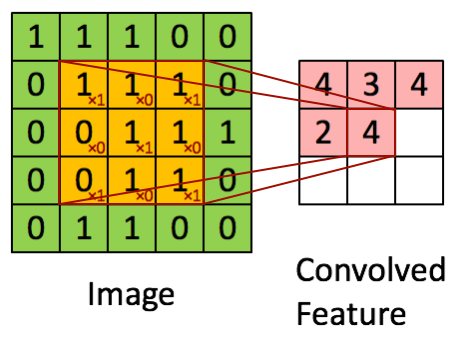
\includegraphics[scale=0.55]{figures/cnn-ex1.png}
  \caption{Convoluting a 5x5x1 image with a 3x3x1 kernel to get a 3x3x1 convolved feature. Figure extracted from \cite{CNN-TDS}}
  \label{fig:cnn-ex1}
\end{figure}

\newpage
The neurons in the convolutional layers are then arranged into feature maps. As ANN did, every neuron is connected to a neighborhood of neurons in the previous layer via a set of trainable weights. Inputs are then convolved following these weights in order to compute a new feature map which will be finally sent to an activation function.  
The $k$th output feature map $Y_{k}$ can be computed as \cite{CNN-1}: 
$$ Y_{k} = f(W_{k} * x) $$ 
where $f()$ is the nonlinear activation function, $W_{k}$ is the convolutional filter related to the kth feature map and $x$ the input image. 


\subsection{Pooling layers} \label{sec:pooling-layers}
Another novelty compared to traditional neural network is the pooling layers. Pooling layers have a dimensionality reduction function to decrease the computational power required to process the data. Same as convolutional layers, reducing dimensionality is a way to detect patterns. The two most known and used pooling types are max pooling and average pooling. Their names are very explicit. Max Pooling returns the maximum value from the portion of the image covered by the filter while average pooling returns the average of all the values from the portion of the image covered by the filter. 

But which type of pooling is better? Should I use average or max pooling? Initially, the most common choice was the average pooling. This method smooths out the image and hence the sharp features may not be identified when this pooling method is used. Hence, average pooling simply performs dimensionality reduction as a noise suppressing mechanism by measures the mean value of existence of a pattern in a given region. 

On the other hand, max pooling discards the noisy activations altogether and also performs de-noising along with dimensionality reduction. This method is then sensitive to existence of some pattern in pooled region and roughly says "this type of feature was detected in this general area".

Therefore, there is no pooling method better than an other. The choice of pooling operation is made based on the data.  

\begin{figure}[h]
  \centering
  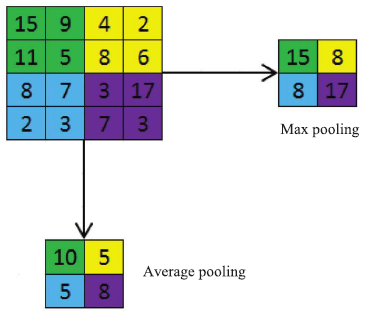
\includegraphics[scale=0.7]{figures/averageVSmaxPOOLING.png}
  \caption{Average pooling vs Max pooling. Figure extracted from \citep{CNN-1}.}
  \label{fig:avgVSmaxPOOLING}
\end{figure}

\newpage
\subsection{Fully connected layers} \label{sec:fully-connected-layer}
Now that we can detect these high level features thanks to the convolutional and pooling layers, the fully connected layer follows to interpret these feature representations. The structure of the fully connected layer is the same as a MLP: every neuron in one layer is connected to every neuron in another layer. The way this fully connected layer works is that it looks at the output of the previous layer (which as we remember should represent the activation maps of high level features) and determines which features most correlate to a particular class by mostly using the \textit{Softmax} classification technique.
The softmax classifier is defined: 
$$ L = \frac{1}{N} \sum_{i=1} L_{i} =  \frac{1}{N} \sum_{i = 1} - log \left(  \frac{e^{f_{yi}}}{\sum_{j=1}^K e^{f_{j}}}  \right) $$ 
where $x_{i}$ is the $i$th input feature with corresponding label $y_{i}$, $K$ the number of classes, $N$ the amount of training datas and $f$ the softmax function defined by: 
$$ f_{j}(z) = \frac{e^{z_{j}}}{\sum_{k} e^{z_{k}}} $$ where $z$ is a vector of arbitrary real-valued scores. 

Therefore, it is at fully connected layers that the model is classifying the image and gives the prediction of what is represented in with a certain probability computed using weights.

% https://adeshpande3.github.io/A-Beginner%27s-Guide-To-Understanding-Convolutional-Neural-Networks/ 

% https://towardsdatascience.com/a-comprehensive-guide-to-convolutional-neural-networks-the-eli5-way-3bd2b1164a53

% SVM vs Softmax : http://cs231n.github.io/linear-classify/ 


% \subsection -> training, backpropagation ? 

\newpage
\section{Support Vector Machine} \label{sec:svm}
Support vector machines (SVM) are supervised learning models that are efficient to resolve classification problems or regression problems\footnote{Defined in \autoref{sec:categories-ML}}. Basically, in the first case, we talk about \textit{support vector classification} (SVC) while we talk about \textit{support vector regression} (SVR) in the second case. SVM is based on the idea of finding an \textbf{hyperplane} that best separates the features into different domains. 

\subsection{Data structure and linearity}
The most known type of SVM is the \textit{linear kernel SVM} which the separation between the different domains is a straight line (or hyperplane if working in multidimensional plans). Nevertheless, it is the very basic case which is only usable for data which are linearly separable (as the example shown in \autoref{fig:classification-regression}) but not for non-linear data. In this case, in 1992, Bernhard E. Boser, Isabelle M. Guyon and Vladimir N. Vapnik suggested a way to create nonlinear classifiers by applying the \textbf{kernel trick} to \textbf{maximum-margin hyperplanes} \cite{wiki-svm}. 

\subsubsection{Margin maximisation}
Maximising the margin, which corresponds to the distance between the closest points (also called \textit{support vector points}) and the hyperplane, can be interpreted as maximising the confidence of the model. In other words, more the SV points is far from the hyperplane, more is the probability of correctly classifying the points in their respective region or classes. Therefore, we can denote the importance of the SV points positions which has an direct impact to the hyperplane. 

As a reminder for the simplest case, given $a \in \mathbb{R}$ the slope and $b \in \mathbb{R}$ the $y$-intercept, the equation form of a linear separation $y$ is:  
\begin{align} \label{eq:1}
y = ax + b
\end{align}

Concerning the hyperplane $\pi$, given $x$ an input vector, $w$ the margin width and $b$ the bias, the form of equation defining the decision surface separating the classes is a hyperplane $\pi$ of the form: 
\begin{align} \label{eq:2}
\pi \equiv w^\top x + b = 0
\end{align}

Moreover, we can define $\pi_{1}$ as the hyperplane of the first class $y^{-}$ (green) parallel to the decision border hyperplane $\pi$ and $\pi_{2}$ as the hyperplane crossing the SV point of the second class $y^{+}$ (red) parallel to $\pi$. The margin is then defined by $\pi_{2}-\pi_{1}$. Knowing the hyperplane defined by \autoref{eq:2}, we can define $\pi_{1}$ and $\pi_{2}$ as: 
\begin{align} \label{eq:3}
\pi_{1} \equiv w^\top x + b = -1 \\
\pi_{2} \equiv w^\top x + b = 1
\end{align}

By solving algebraically $\pi_{2}-\pi_{1}$, we obtain:
\begin{align}
\pi_{2}-\pi_{1} &= (w^\top x + b - 1) - (w^\top x + b + 1)\nonumber  \\ 
 				&= \frac{2}{\mid w \mid} \nonumber
\end{align} 

Thus, to increase the margin, we have to minimize $\mid w \mid$. In other words, with the condition that there are no datapoints between $\pi_{1}$ and $\pi_{2}$:
\begin{center}
$ x_{i} \cdot w + b \geq +1 \Rightarrow y_{i} = +1 \Rightarrow y^{+} $ \\
$ x_{i} \cdot w + b \leq -1 \Rightarrow y_{i} = -1 \Rightarrow y^{-} $
\end{center}

The following pseudo-code sums up the procedure, so either we save the $w$ and $b$ values and keep going or we adjust the parameters, which corresponds to a convex optimization problem which surely gives us global minimum value, and keep going. Moreover, \autoref{fig:margin-svm} illustrates the problem and all the variables. 
 
\begin{algorithm} 
  \caption{Margin Maximization - Finding the best hyperplane} \label{alg:max-margin}
  \begin{algorithmic}[1]
  \ForAll {point $x_{i}$ we check:}
  \If {$y_{i} \cdot (w \cdot x_{i} + b) = 1$}
  \State $x_{i} =$ SV point
  \State Correctly classified $\Rightarrow$ Save parameters $b$ and $w$ 
  \ElsIf {$y_{i} \cdot (w \cdot x_{i} + b) > 1$} 
  \State Correctly classified $\Rightarrow$ Save parameters $b$ and $w$
  \Else 
  \State Incorrectly classified $\Rightarrow$ Adjust parameters $b$ and $w$
  \EndIf 
  \EndFor
  \end{algorithmic}
\end{algorithm}



% http://web.mit.edu/6.034/wwwbob/svm-notes-long-08.pdf
% https://medium.com/deep-math-machine-learning-ai/chapter-3-support-vector-machine-with-math-47d6193c82be 

\begin{figure}[h]
  \centering
  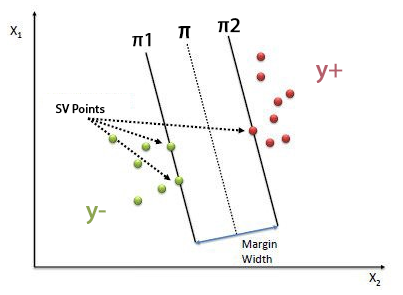
\includegraphics[scale=0.85]{figures/margin-svm.png}
  \caption{SVM hyperplane and margin representation. Figure extracted from \cite{svm-towardsdatascience}.}
  \label{fig:margin-svm}
\end{figure}

\newpage
\subsubsection{Kernel trick}
Let's now define the kernel trick and how does it work. Basically, the kernel trick is used by a \textit{radial basis function} (RBF) SVM where this trick will allow us to use a linear classifier to resolve a non-linear problem by transforming data into another higher dimension (potentially infinite) that has a clear dividing margin between classes of data. The kernel trick is then a way of computing the scalar product of two vectors $x$ and $y$ in some (very high dimensional) feature space. \\

More formally, given an input vector $x$ labelled by $y$. We apply a non-linear transformation $\phi : \mathbb{R} \rightarrow H$ to the data where $H$ is an \textit{Hilbert space}\footnote{An \textit{Hilbert space} is a real vectorial space including a scalar product, which allow us to measure lengths, angles and to define an orthogonality.}. After this transformation, the procedure only depends of the scalar product $\phi(x) \cdot \phi(y)$  but computing this scalar product in a high-dimensional space is somehow complicated. The idea of the kernel trick is then to use a kernel function $K$ of the form: $K(x,y) = \phi(x) \cdot \phi(y)$. Simply, applying kernel trick means just to the replace scalar product of two vectors by the kernel function.\\ 
       
% est-ce que je dois expliquer comment ça marche ?

% https://scikit-learn.org/stable/auto_examples/svm/plot_rbf_parameters.html
Concerning RBF SVM, the kernel function is defined as: 
$$ K(x,y) = exp( - \gamma \norm{x-y}^2 ) $$
where $\gamma$ defines how far the influence of a single training example reaches, with low values meaning "far" and high values meaning "close". Moreover, RBF SVM implies a cost  parameter $c$ which defines a penalty value when a datapoint is not correctly classified. For larger values of $c$, a smaller margin will be accepted if the decision function is better at classifying all training points correctly. A lower $c$ will encourage a larger margin, therefore a simpler decision function, at the cost of training accuracy. 

\begin{figure}[h]
  \centering
  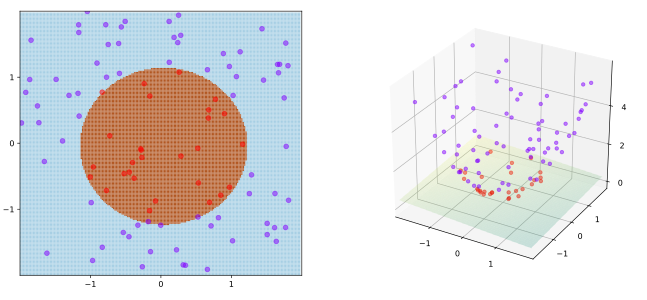
\includegraphics[scale=0.65]{figures/kernel-trick.png}
  \caption{A training example of SVM with kernel given by $\phi((a, b)) = (a, b, a^{2} + b^{2})$ and thus goes from a 2D space to a 3D space defined by $K(x, y) = x \cdot y + x^2 y^2$. The training points are mapped to a 3-dimensional space where a separating hyperplane can be easily found. Figure extracted from \cite{wiki-svm}.}
  \label{fig:kernel-trick}
\end{figure}

\newpage
\section{Evaluation and validation} \label{sec:evaluation}
% \textit{\textbf{Plan:} maitrise d'évaluation, parler du pourcentage de précision, comment on évalue la classification? comment on entraine? comment on valide?}
% parler de crossvalidation, overfit, 
% Confusion matrix -> TP, FP etc 
% ROC Curves
 
Once classification models are done, it is mandatory to evaluate the prediction to determine potential errors that should falsify the obtained results.  To do that, it is useful to know which type of error exist and how are we computing the performance of a classification model to finally validate the prediction or not. More precisely, we call the statistical measures of the performance of a binary classification test "sensitivity" and "specificity". 

\subsection{Sensitivity, specificity and confusion matrix}
A confusion matrix is an $N \times N$ matrix that is often used to summarize the performance of a classification model. The confusion matrix gives information about what the model is predicting right and what error it did. These two informations are separated in 4 categories: True Positive (TP), True Negative (TN), False Positive (FP) and False Negative (FN). The two first one are the results where reality is in favor with the model predictions while FP and FN define the two types of errors that the model can encounter.

Given the confusion matrix, we can compute the accuracy of the model to show how often the classifier was correct following this formula: 
$$ accuracy = \frac{TP + TN}{TP + TN + FP + FN} $$
A variant of accuracy is the Positive Predicted Value (PPV), also called \textit{precision}, that computes how often the model was correct when it predicted positively: 
$$ precision = \frac{TP}{TP + FP} $$ 

The two other values interesting to compute are the \textbf{sensitivity} and \textbf{specificity} of the model. 

The sensitivity, also called \textit{true positive rate} or \textit{recall}, shows how often the model correctly detect a true response while it is the case. It increases by reducing the number of FN. When the number of FN is null, it means that the positive response of the model is always verified. Likewise, a negative response asserts that the positive case is impossible. In summary, when the model has a 100\% sensitivity, it means that the model is predicting perfectly. Mathematically, the sensitivity is computed by: 
$$ sensitivity = \frac{TP}{TP + FN} $$ 

The specificity, also called \textit{true negative rate}, is simply the opposite of sensitivity. It shows how often the model predicted negatively when the response in reality is negative too. Similarly, the specificity is increased by reducing the number of FP.
$$ specificity = \frac{TN}{TN + FP} $$ 


Moreover, it exists a value, called {F1 score}, that combines recall and precision which indicates the weighted average of both elements. It is usually used to rate classifier performance and hence take into account FP and FN. 
$$ \text{F1 score} = \frac{2*recall*precision}{recall+precision} $$

\subsubsection{Application} \label{sec:appli-confusion-matrix}
To illustrate these terms and the use of the confusion matrix, let's take an example of a medical testing where the model is trying to predict if a patient has a disease or not. Roughly, there exist 4 possible results and evaluations: 
\begin{center}
    \begin{tabular}{cl}
      TP & the patient has the disease and the test is positive\\
      TN & the patient does not have the disease and the test is negative \\
      FP & the patient does not have the disease but the test is positive \\
      FN & the patient has the disease but the test is negative \\
    \end{tabular}
\end{center}

Taking a sample of 100 people, the current model predicts 20 people to have the disease but only 15 people have actually disease and among those 15 people, the model predicted 12 correctly. These results put in the confusion matrix gives what is illustrated in \autoref{fig:confusion-matrix}. 

Moreover, we can compute the different values tackled previously to evaluate the model. 

\begin{center}
    \begin{tabular}{|c|c|}
      \hline 
      accuracy & 89\% \\
      \hline
      precision & 60\% \\
      \hline
      sensitivity & 80\% \\
      \hline
      specificity &  90\% \\
      \hline
    \end{tabular}
\end{center}

\begin{figure}[h]
  \centering
  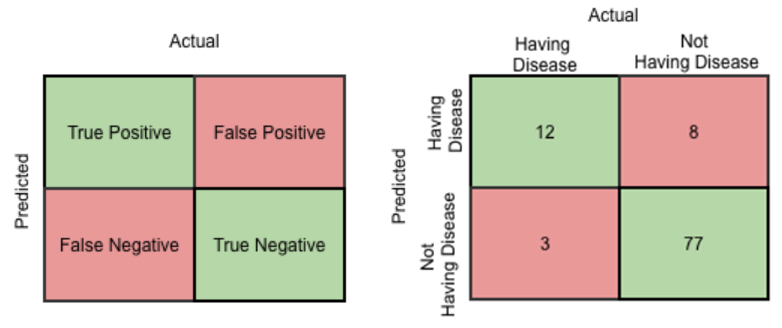
\includegraphics[scale=0.4]{figures/confusion-matrix.png}
  \caption{A confusion matrix prototype and an application to the above example. $TP = 12$, $FP = 8$, $TN = 3$, $TN = 77$.}
  \label{fig:confusion-matrix}
\end{figure}


\subsection{ROC curves}
The \textit{Receiver Operating Characteristic} curve (ROC curve) is a plot of the true positive rate (TPR, sensitivity) against the false positive rate (FPR, corresponding to 1-specificity) for different classification thresholds. In other words, ROC curves can be used to select a threshold for a classifier which maximizes the TP while minimizing the FP. A perfect ROC curve would follow the two axes. In general, real-life classification rules produce ROC curves which lie between these two extremes. 

Given a ROC curve, it is interesting to compute what we call the \textit{Area Under The Curve} (AUC) which represents the degree or measure of separability, i.e. how much the model is capable of distinguishing between classes. If $AUC = 1$, it means that the test has perfect accuracy. 

For instance, in the example tackled above in \autoref{sec:appli-confusion-matrix} , higher the AUC is, better the model is at distinguishing between patients with disease and patients with no disease.

\begin{figure}[h]
  \centering
  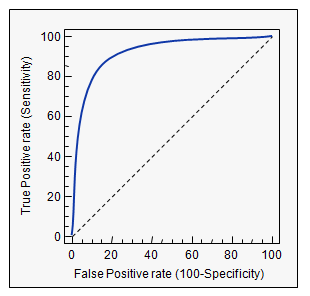
\includegraphics[scale=0.8]{figures/roc-curve.png}
  \caption{A ROC curve. The blue line denotes the change of TPR with different FPR for a model. The AUC is described by the area under this blue line. Figure extracted from \cite{roc-schema} }
  \label{fig:roc-curve}
\end{figure}

\newpage
\subsection{Overfit, underfit and cross-validation}
%OVERFIT + UNDERFIT & CROSS VALIDATION section à faire si possible
A frequent problem in model training is when the fitting is too low or too high which implies a lack of information or in contrary a too large value of information to learn which may lead to noise. The first case is called \textit{underfitting} while the second case is called \textit{overfitting}. Finding a happy medium is then an important case to manage. This value is also called \textit{goodness of fit} which refers to how closely a model's predicted values match the observed (true) values.

\begin{figure}[h]
  \centering
  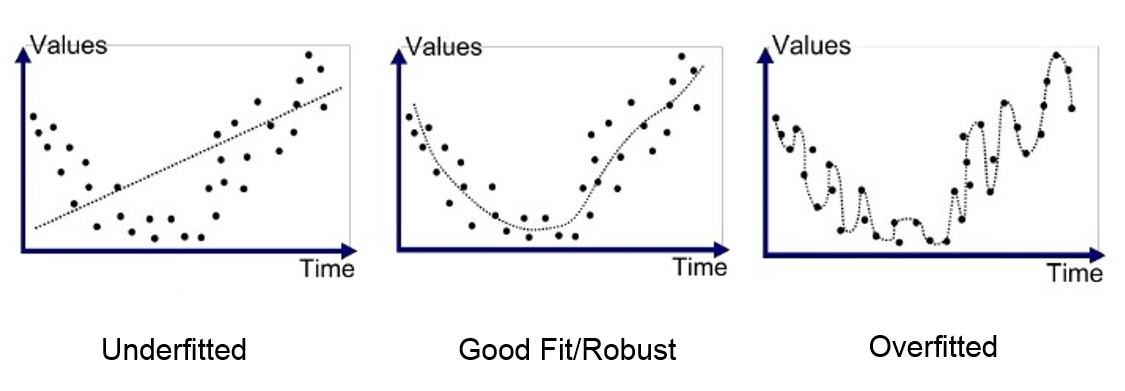
\includegraphics[scale=0.35]{figures/over-under-fit.png}
  \caption{Illustration of an underfit, a good fit and an overfit. Figure extracted from \cite{over-under-fit-schema} }
  \label{fig:over-under-fit}
\end{figure}

\subsubsection{Overfitting}
Generally, more you learn, the better it is. But in case of learning to predict, it can cause troubles. Why would learn a large number of information/features be a bad thing? 
The objective is to find a model that \textbf{generalizes} well certain patterns to finally apply these generalisations to new data. Therefore, while learning too much data, the model may save too much superfluous and too detailed information which are only specific to the images that the model is currently learning. In other words, the predictive model will capture the generalizable correlations and the \textbf{noise} produced by the data.

In summary, we can define overfitting as a model that is too specialized on training set data and that will not generalize well. That implies that the model will predict very well on training set data but bad on new datasets. Therefore, to detect overfitting, we see if the model predict much better on the training set (used to learn) than on the test set (that is never touched before prediction), if it is the case, then we are likely overfitting.


\subsubsection{Underfitting}
Underfitting problem is more meaningful to everyone. This is exactly the contrary to overfitting which means that not enough information are learnt to predict new datasets correctly, even for the training set. In this case, the model suffers from a large bias and then will not be viable for any dataset. 


\subsubsection{Cross-validation}
To prevent those problems, cross-validation (fully called \textit{k-fold cross-validation}) is one of the most known method which is estimating the skill of machine learning models. In standard $k$-fold cross-validation, we partition the data into $k$ subsets, called folds. Then, we iteratively train the algorithm on $k-1$ folds while using the remaining fold as the test set. In other words, one round of cross-validation involves partitioning a sample of data into complementary subsets, performing the analysis on one subset (called the training set), and validating the analysis on the other subset (called the validation set or testing set) \cite{wiki-cross-validation}. This way, we generate multiple mini train-test splits (then, the training tests number) from the initial training data to multiply the chance to detect and prevent from over or underfitting.

The choice of $k$ is usually 5 or 10. But as $k$ gets larger, the difference in size between the training set and the resampling subsets decreases which implies the reduction of the bias of the technique.

Of course, cross-validation is not the only way to prevent from over and underfitting. There exists much solutions such as simply train with more data or remove some features. 


\begin{figure}[h]
  \centering
  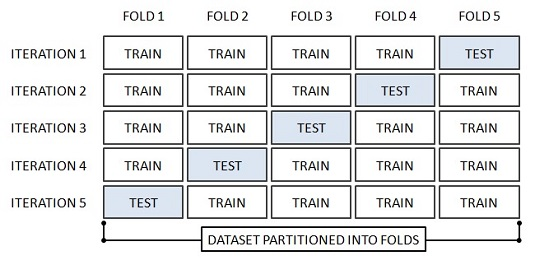
\includegraphics[scale=1.3]{figures/cross-validation.jpg}
  \caption{Illustration of 5-fold cross-validation. Figure extracted from \cite{MachineLearningForDummies}.}
  \label{fig:over-under-fit}
\end{figure}


\chapter{A well-known application: breast cancer detection} \label{chap:breast-cancer}
One of the most recurrent serious disease which is one of the leading for women globally is breast cancer. To overcome this disease, mammography is one of the important methods which use medical imaging to detect breast cancer. This chapter is devoted to the state-of-the-art of the article "Breast cancer detection using deep convolutional neural networks and support vector machines" \cite{breast-cancer} written by Dina A. Ragab, Maha Sharkas, Stephen Marshall and Jinchang Ren published recently in January 2019. We will study the methodology adopted by the authors to detect breast cancer through magnetic resonance imaging and present the results that they have obtained. These results are obtained using the digital database for screening mammography (\textbf{DDSM}) and the Curated Breast Imaging Subset of DDSM (\textbf{CBIS-DDSM}) that are publicly available datasets.

\section{Biological features}
% voir page 5 du 2e article sur breast cancer 
To detect breast cancer, it is essential to detect the indicators of it, i.e. tumors. Globally, the two most important and most significant signs of the disease are \textit{masses} and \textit{microcalcifcations} (MCs).  

\begin{defn}
A mass is a lump in the body and may be caused by the abnormal growth of cells, a cyst, hormonal changes, or an immune reaction. It can be either benign or malignant \cite{NCI}.
\end{defn}  

\begin{defn}
A MC is a tiny deposit of calcium in the breast that cannot be felt but can be detected on a mammogram. A cluster of these very small specks of calcium may indicate that cancer is present \cite{NCI}. Same as masses, MCs can either be benign or malignant.  
\end{defn}

\subsection{Benign and malignant tumors}
In two words, the difference between benign and malignant tumors is that the meaning of malignant is cancerous and the meaning of benign is non-cancerous but they have each one specific features. The benign tumors won't invade nearby tissues or spread to other areas of the body and are characterized for breast cancer detection by round or oval shapes. Nevertheless, even if at the start they are non-cancerous, it may lead to malignant tumors which denotes the importance of removing it. 

On the other hand, malignant tumors can invade nearby tissues. In the case of breast cancer, the tumor begins in breast tissue but could spread to lymph nodes which may lead the cancer cells to other areas of the body, like the liver or bones. In this case, the malignant tumors are characterized by partially rounded shape with an irregular outline and will appear whiter than any tissue surrounding it.

\begin{figure}[h]
  \centering
  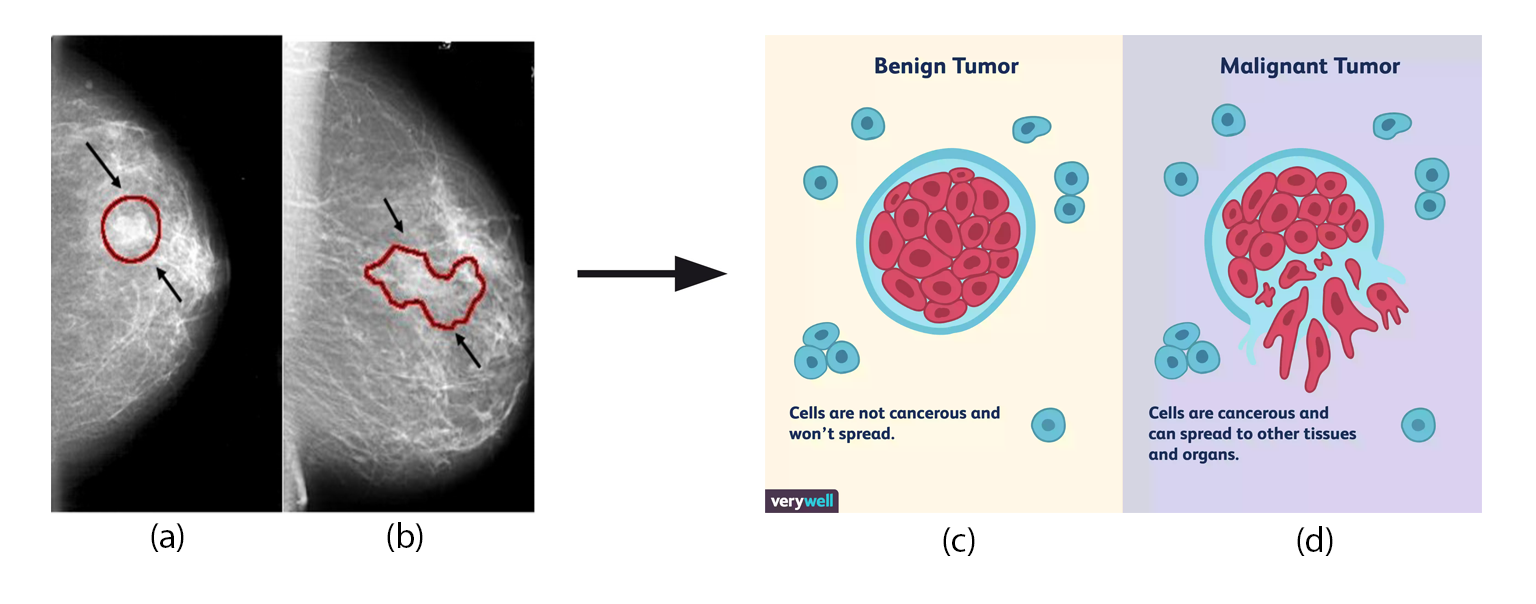
\includegraphics[scale=0.28]{figures/tumor-types.png}
  \caption{Illustration of the different types of tumor. (a) Mass, (b) MCs, (c) Benign, (d) Malignant. First, the tumor can be masses or MCs and no matter what type, they are either benign or malignant. (a) and (b) images are from \cite{breast-cancer} and (c) and (d) from Joshua Seong \copyright Verywell, 2017.}
  \label{fig:tumor-types}
\end{figure}

Therefore, the purpose of the work of Ragab et al. \cite{breast-cancer} is to detect the masses and to classify benign and malignant tissues in mammograms. The methodology to do that is presented in the next section.  

\section{Methodology for breast cancer detection}
The methodology tackled in the paper \cite{breast-cancer} is divided into 5 main steps: (1) image enhancement, (2) image segmentation, (3) feature extraction, (4) feature classification, and finally, (5) an evaluation for the classifier. 

The functions and the methods applied for these steps make subject of the next subsections. Basically, the objective is to detect the region of interest (ROI) of the image to extract and classify the features that would indicate if the disease is present or not. 

\subsection{Image enhancement} \label{sec:img-enhancement-breast}
Taking a mammogram image in input returned by magnetic resonance imaging, the first step consists to suppress the noise to make the image more clear to highlight potential anomalies. To do that, the authors of the paper are using \textit{contrast-limited adaptive histogram equalization} (CLAHE) which is a type of \textit{adaptive contrast enhancement} (AHE) will be used to improve the contrast in images.  

The CLAHE technique is characterized by these following steps \cite{breast-cancer}: 
\begin{enumerate}
\item Divide the original image into contextual regions of equal size. \\
	  $\rightarrow$ \textit{Contextual regions} are relevant regions depending on neighbourhood pixels. For example, if we take a region of size 2x2, it is quite hard to extract information from that. The difficulty is then to find regions' sizes which may help.   

\newpage	  
\item Apply the histogram\footnote{An \textit{histogram} is an accurate representation of the distribution of numerical data. (Wikipedia)} equalization on each region \\ 
	  $\rightarrow$ \textit{Histogram equalization} is a method in image processing of contrast adjustment using the image's histogram characterized by the following equation \cite{book-digital-processing}: 
	  $$ g_{i,j} = floor((L-1) \sum_{n=0}^{f_{i,j}} p_{n}) $$ where $g$ is the histogram equalized image, $L$ is the number of possible intensity values, $f$ the image and $p$ the normalized histogram computed by $p_{n} = \frac{\text{pixel numbers with intensity n}}{\text{total number of pixels}}$. 
	  
\item Limit this histogram by the clip level (which corresponds to the threshold level to determine how the clipping occurs) 

\item Redistribute the clipped amount among the histogram to be as close as possible to the desired histogram

\item Obtain the enhanced pixel value by the histogram integration. 
\end{enumerate}

\begin{figure}[h]
  \centering
  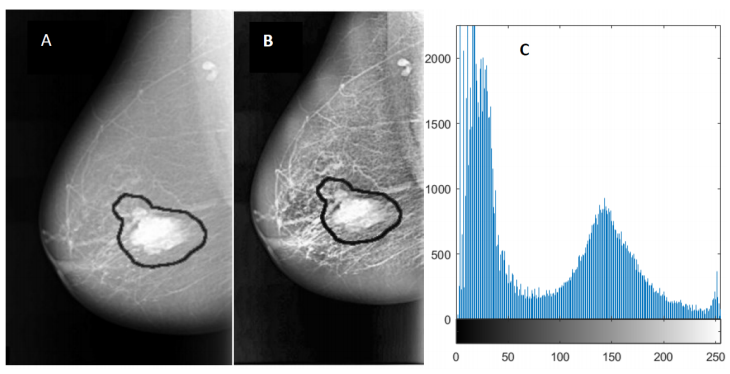
\includegraphics[scale=0.55]{figures/CLAHE.png}
  \caption{Mammogram enhancement using CLAHE. (A) Original malignant mass case extracted from DDSM,(B) Enhanced image using CLAHE, and (C) Histogram representation of the image. Figures extracted from \cite{breast-cancer}}
  \label{fig:CLAHE}
\end{figure}

\subsection{Image segmentation}
After the enhancement of the image done, the next step is to segment the image into different regions which have similar features and properties. This segmentation can for example be done by using ANN, which is presented in \autoref{sec:neural-networks}. The methods used in the paper are thresholding and region-based methods in addition to CNN tackled in \autoref{sec:CNN} to extract the region of interest (ROI). The tumors in the DDSM dataset are labelled with a red contour and accordingly, these contours are determined manually by examining the pixel values of the tumor and using them to extract the ROI \cite{breast-cancer}.

\subsubsection{Thresholding method}
Thresholding is the simplest method of image segmentation and usually used to transform an image into binary images\footnote{Warning: binary images are not grey-scale images. In binary images, only 2 values are possible for each pixel: black or white.} (black and white images). As its name said, the thresholding method is based on a threshold value $T$ which will determine if a pixel is 0 (white) or 1 (black) in the output image $p(x,y)$ for every pixel of the original image $q(x,y)$. Formally: 
$$
q(x,y) = \left\{
    \begin{array}{ll}
        1 & \mbox{if } p(x,y) > T \\
        0 & \mbox{else if } p(x,y) < T
    \end{array}
\right.
$$
In our case, thresholding method is used to determine the tumor region by a threshold value which is a value determined with respect to the red color pixel. After some trials, the threshold was set to 76 for all the images regardless of the size of the tumor \cite{breast-cancer}.

\subsubsection{Region-based method} 
Region-based method divides an image into different regions based on pre-defined criteria (color, intensity, etc). The main advantage of this method is that it is noise resilient. The method is defined by two types of algorithms: (1) region growing and (2) region splitting and merging. Thus, after the thresholding method which returns the biggest area within this threshold along the image, region-based method is used to crop automatically the tumor. 

\begin{itemize}
\item \textbf{Region growing:} also classified as a pixel-based image segmentation, region growing algorithm is based on a single pixel called \textit{seed pixel} and checks the neighboring pixels and add them to the region if they are similar to the seed. This last is repeated for each of the newly added pixels and is stopped if no more pixels can be added. Thus, these adding steps are making the region growing. 

\item \textbf{Region splitting and merging:} the image is successively split into quadrants based on a homogeneity criterion and regions that possess similarities regarding this criterion are merged to create the segmented result. All regions are then compared with its neighbours to compute their homogeneity and merged with them if the region pass the homogeneity test. The process is repeated until all regions pass this homogeneity test. The region splitting and merging is somehow the opposite of the region growing algorithm. 
\end{itemize} 

\subsubsection{Image segmentation summary}
The methodology used by Ragab et al. is then summarized by these following steps combining CNN, threshold and region-based techniques \cite{breast-cancer}: 
\begin{enumerate}
\item $\left[\text{Threshold}\right]$\footnote{The [] indicates the technique used for this step.} Convert the original mammogram grayscale image into a binary image. 
\item $\left[\text{CNN}\right]$ Binary image objects are labelled and the number of pixels are counted. 
\item $\left[\text{Threshold \& region-based}\right]$ All binary objects are removed except for the largest one, which is the tumor with respect to the threshold. The largest area is the area enclosed within the red contour labelled around the tumor. 
\item $\left[\text{Threshold}\right]$ After the algorithm checks all pixels in the binary image, the largest area pixels within the threshold are set to 1, otherwise all other pixels are set to 0
\item The resulting binary image is multiplied with the original mammogram image to get
the final image without taking in account any useless information in the image.
\end{enumerate}


\begin{figure}[h]
  \centering
  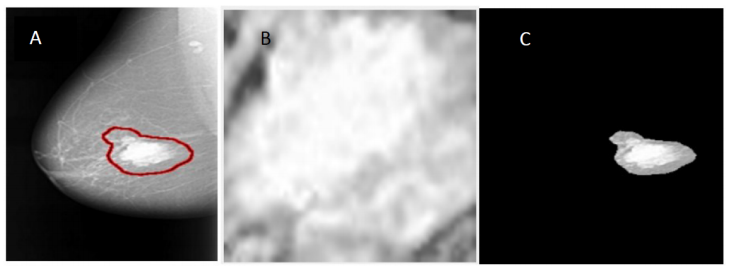
\includegraphics[scale=0.6]{figures/image-segmentation.png}
  \caption{Image segmentation using above methodology. (A) Original malignant mass case extracted from DDSM, (B) enhanced ROI extracted manually using circular contours, and (C) enhanced ROI extracted automatically by the region based method. Figures extracted from \cite{breast-cancer}.}
  \label{fig:image-segmentation}
\end{figure}


\subsection{Feature extraction}
The next step after image enhancement and segmentation is to extract features from these preprocessed images. To do that, CNN is the most used common and used method of the recent years. Different types of CNN architectures exist such as CiFarNet, the Inception v1 (GoogleNet) or AlexNet. This last is the one chosen by the authors from its performance that has been proved better over the other deep learning methods for image recognition by reducing the top-5 error from 26\% to 15.3\%. 

\subsubsection{AlexNet architecture}
AlexNet architecture is defined by 5 convolution layers, 3 pooling layers, and 2 fully connected layers with approximately 60 million free parameters. As reminder, the function of these different types of layers is explained in \autoref{sec:CNN}. Concerning the activation function, AlexNet uses Rectified Linear Units (ReLUs) defined by $f(x) = max(0, x)$ which turns every negative values to zero. 

\begin{figure}[h]
  \centering
  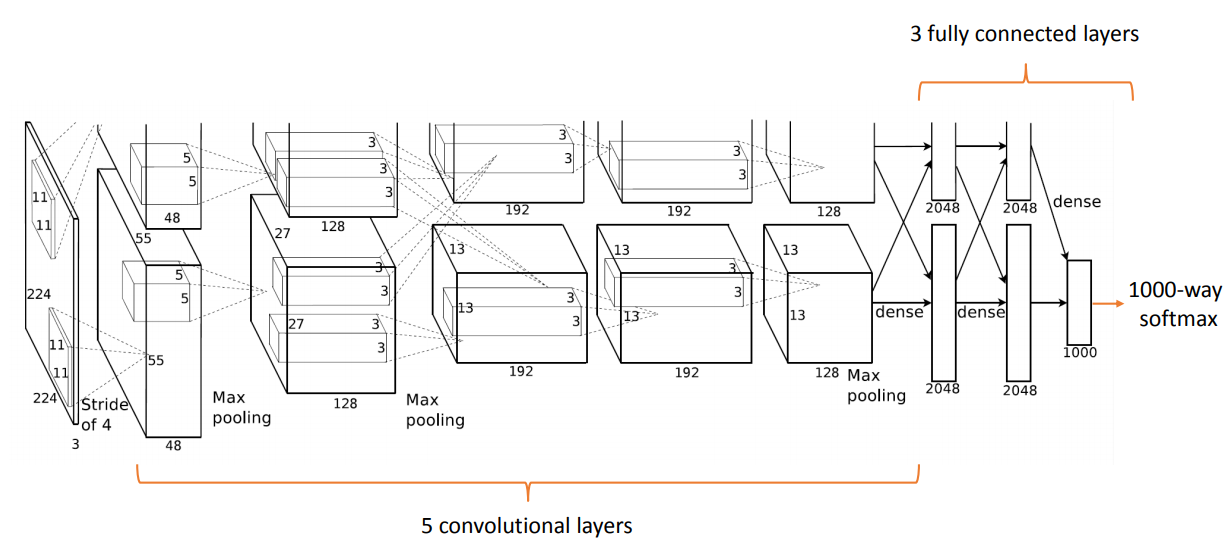
\includegraphics[scale=0.47]{figures/AlexNet.png}
  \caption{Illustration of AlexNet architecture. Figure extracted from \cite{AlexNet}.}
  \label{fig:image-segmentation}
\end{figure}

\subsubsection{Types of features}
There exists different types of features to extract in a mammogram image. Here are a non-exhaustive list of these different features types \cite{breast-cancer-2}: 
\begin{itemize}
\item \textbf{Contrast features:} this feature's type captures how well a lesion is separated from the background. An important nuisance in this setting is the tissue surrounding the lesion in addition to its border sharpness computed by the acutance feature and margin contrast. 

\item \textbf{Texture features:} a sign that may indicate the presence of a tumor is the non-presence of holes in the candidate lesion. Indeed, linear structures within a lesion can indicate an unfortunate projection rather then cancer \cite{breast-cancer-2}. 

\item \textbf{Geometrical features:} regularity of the border of a lesion is often used to classify lesions. The authors of \cite{breast-cancer-2} have incorporated 5 topology descriptor that may help to detect the disease. These are eccentricity, convexity, compactness, circular variance and elliptic variance \cite{breast-cancer-2}. 
\end{itemize}

Moreover, note that there exists other feature's type that are not related to the mammogram image. For instance, location features indicate the locations that are more sensible to the occurrence of lesions such as lymph nodes or patient features such as his age. 


\subsection{Classification}
The breast cancer detection has obviously two different possible outputs regarding the lesion. The ROI is classified as either \textbf{benign} or \textbf{malignant} according to the features. To classify this type of data, there exists many methods such as ANN, binary decision tree or SVM. This last has proven its efficiency for breast cancer detection by achieving high classification rates. That is the reason why the authors of the paper are using it. SVM method is fully explained in \autoref{sec:svm}.  

To do that, after the training step, the last fully connected layer is replaced by a new layer for the classification of these two classes: benign and malignant masses.

\subsection{Evaluation}
Finally, the last step of the classification is the evaluation. We have seen in \autoref{sec:evaluation} different tools and methods to evaluate a classifier. All these tools are appropriate to use in order to get an accurate classifier to make potential modification to enhance the model if necessary. The evaluation results of Ragab et al.'s model make subject of the next section. 

A global summary of the methodology is presented in the \autoref{fig:summary-breast-cancer-methodology}.

\newpage
\hspace*{0mm}\vfill
\begin{figure}[h]
  \centering
  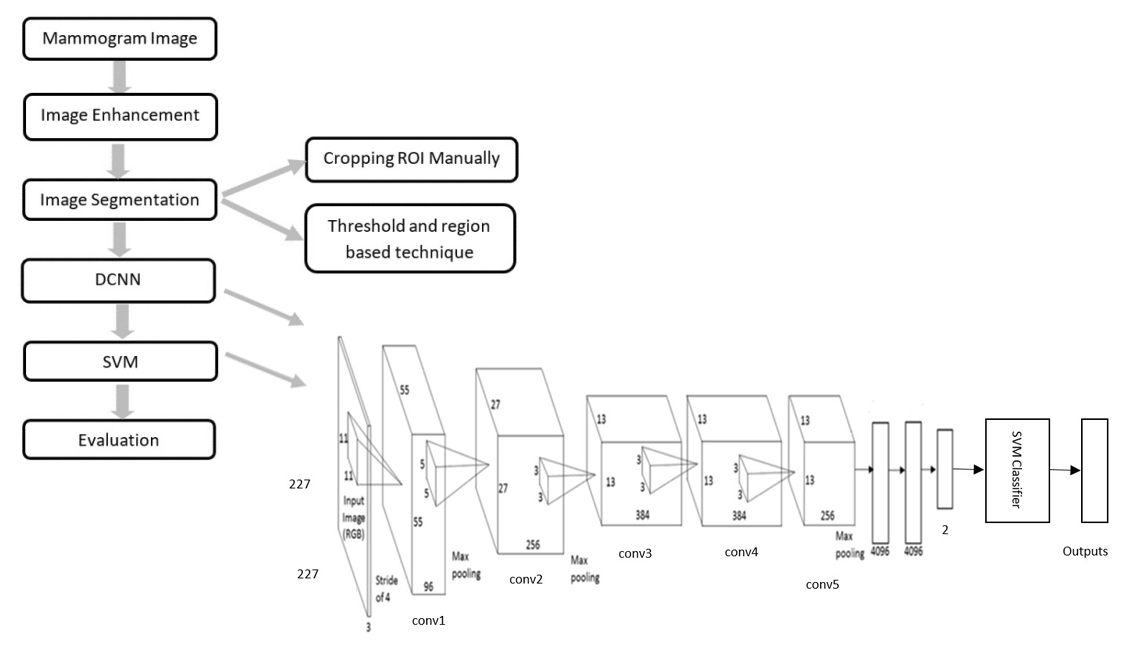
\includegraphics[scale=0.375]{figures/summary-breast-cancer-methodology.png}
  \caption{Summary of the breast cancer detection methodology of Regab et al.'s paper \cite{breast-cancer}.}
  \label{fig:summary-breast-cancer-methodology}
\end{figure}
\vfill\hspace*{0mm}

\newpage
\section{Current results}
The following results are obtained by taking samples from the DDSM dataset which contains images that have been pre-processed and converted to 299x299 images by extracting the ROIs. The entire dataset contains 55,890 training examples, of which 14\% are positive and the remaining 86\% negative. 70\% of the DDSM samples taken have been used for training and 30\% for testing. This proportion is usually used when doing a classification problem. 

The first steps are images enhancement and segmentation. For those steps, the following numbers of training and testing samples were used:
\begin{center}
    \begin{tabular}{|c|c|c|c|}
      \hline
       & Training & Testing & Total \\
      \hline
       DDSM (ROI cropped manually) & 1580 & 676 & 2256 \\
      \hline
       DDSM (ROI using threshold and region based) & 1288 & 552 & 1840 \\
      \hline
       CBIS-DDSM & 3691 & 1581 & 5272 \\
      \hline
    \end{tabular}
    \captionof{table}{The number of training and testing samples for all the datasets used \cite{breast-cancer}.}
\end{center}

Initially, when using manual cropping method for segmentation in addition to CNN to classify, the accuracy of the new-trained AlexNet was only 71.01\%. However, when combining CNN with SVM for the classification, this accuracy increased to 79\% with AUC equals to 0.88 (88\%). As reminder, higher the AUC is, better the model is at predicting malignant as malignant and benign as benign.

Whereas, concerning the thresholding and region-based method for segmentation, the accuracy while using only CNN reached only 69.2\%. Nevertheless, this accuracy was strongly increased and even more than the first method since it achieved 80.9\% with same AUC value. 

The complete evaluation of both methods using SVM with different kernel functions is presented in \autoref{fig:eval-article} by computing the accuracy, AUC, sensitivity, specificity, precision and F1 score. 


In conclusion, the choice concerning the kernel function is unequivocal, the best result was always obtained by using linear kernel functions. Concerning the choice of the segmentation technique, both are viable. Nevertheless, thresholding added to region-based method has slightly a better average accuracy and precision.

\newpage
\hspace*{0mm}\vfill
\begin{figure}[H]
  \centering
  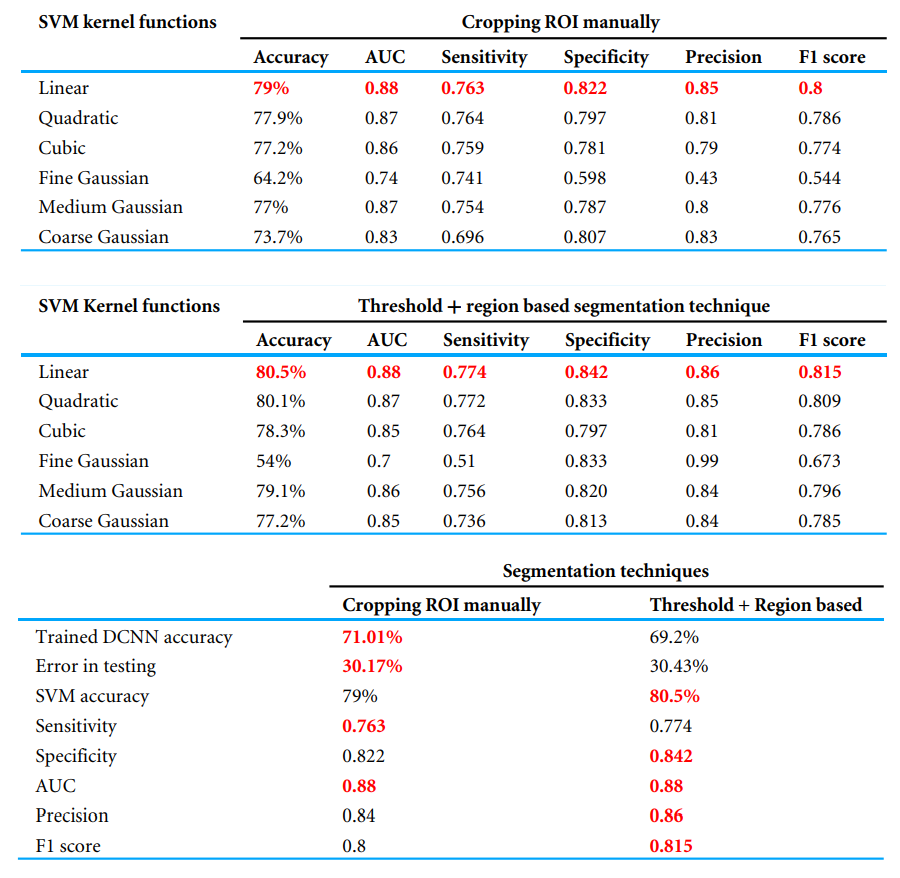
\includegraphics[scale=0.465]{figures/eval-article.png}
  \caption{Complete evaluation of the different methods used. The first results table is obtained by using manual cropping for segmentation while the second one is using thresholding and region-based methods. Moreover, these two first tables are comparing results with different kernel functions for SVM. The last table is summarizing the different evaluation values between these two segmentation methods. A red value indicates the greatest value between the compared methods \cite{breast-cancer}.}
  \label{fig:eval-article}
\end{figure}
\vfill\hspace*{0mm}

%%%%%%%%%%%%%%%%%%%%%%%%%%%%%%%%%%%%%%%%%%%%%%%%%%%%%%%%%%%%%%%%%%
% 								MA2 							 %
%%%%%%%%%%%%%%%%%%%%%%%%%%%%%%%%%%%%%%%%%%%%%%%%%%%%%%%%%%%%%%%%%%

\chapter{Model prototype} \label{sec:CIFAR10-exp}

After discussing theoretically about the different methods and materials of image classification and recognition, this chapter is tackling a simple image classification model implementation for the non-medical dataset CIFAR-10 \cite{CIFAR10} based on the CNN implementation of Jason Brownlee \cite{CIFAR10-implementation-1} and Dan Nelson \cite{CIFAR10-implementation-2}. Henceforth we can determine the parameters which optimize the evaluation criteria of a predictive model and how it reacts to noise. 

\section{The CIFAR10 dataset}
The CIFAR (Canadian Institute For Advanced Research) created two versions of datasets: CIFAR-10 and CIFAR-100 which differs from the number of image classes that contains the respective datasets. In this work, we will use the CIFAR10 dataset whose involves a collection of images belonging to the following 10 classes: airplanes, cars, birds, cats, deer, dogs, frogs, horses, ships, and trucks illustrated in \autoref{fig:cifar10}.  

The CIFAR-10 dataset consists of 60000 $32\times32$ colour images in these 10 classes, with 6000 images per class mutually exclusive. 50000 of these images are dedicated to the training phase and constitutes the training set while the 10000 remaining are dedicated to the evaluation and then shapes the test set (test batch). These 50000 training images are divided into batches of 10000 elements. The training batches contain the remaining images in random order, but some training batches may contain more images from one class than another. Between them, the training batches contain exactly 5000 images from each class.

The fact that the images are in low resolution allows mainly fast training phase execution which makes the testing easier. Moreover, CIFAR-10 is a well-known dataset and has proven several times that it was a friendly and efficient dataset to use in order to test different models on it as well as MNIST dataset which approaches a trivial problem (recognizing 10 digits).       

\section{Model implementation}

In this section, the development of a convolutional neural network using Python3 and its machine learning packages such as TensorFlow and Keras is done. Moreover, parameters used are reviewed in order to optimize the model's accuracy. 

\subsection{Why CNN over other models?} \label{sec:why-cnn}
As seen in \autoref{sec:CNN}, the best model type for images are convolutional neural networks. Some reasons of this efficiency may be that CNN is a kind of deep learning neural network where \textbf{transfer} learning happens which means that learned knowledge about the data are stored and used for the future. An example of transfert learning related to CIFAR-10 would be that the knowledge acquired to recognize cars could be applied when trying to recognize trucks. A simple analogy of transfert learning could be the learning of a Romance (e.g. Spanish) language while your native language is another Romance language (e.g. Italian) facilitates and accelerates the learning. This works the same for machine learning and image recognition.     

Moreover, thanks to its pooling layers (see \autoref{sec:pooling-layers}), CNN manages dimensionality reduction which enhances the feature extraction. Thus, CNN can somehow be thought of automatic feature extractors from the image. In comparison with other methods such as KNN, SVM or logistic regression where we need to spend much time on feature selection, this time is then less significant for CNN.   

\subsection{Structure and implementation}

\subsubsection{Dataset preprocessing}

% Sample 
\textbf{Sampling}

Before starting to create the model, the preprocessing step on dataset is essential in order to get more significant prediction results. Initially, the training set of CIFAR-10 is composed of 50000 images. However, it is necessary to \textbf{sample} this starting training set for two reasons: 
\begin{itemize}
\item To avoid multiple large execution times: multiple tests are done, it would be really long and constraint to train on the whole training set at each execution 
\item To produce highly imbalanced set in order to test the methods on it and obtain significant results
\end{itemize}

Hence, the sampling phase is splitting up the 50000 images into a drastically smaller number. Knowing that the CIFAR-10 is divided into 5 batches of 10000 images, the sample method of our model is simply to use only one batch of the dataset.  \\

%One-hot encoding
\textbf{One hot encoding} 

The second preprocessing to apply on the dataset is a process called \textbf{One hot encoding}. What is this doing is converting the categorical data label encoding (i.e. airplanes=0, cars=1, birds=2, ...) into another type of encoding that enhances the reading of these data by the machine learning algorithms. But why this label encoding would not be enough?  The problem with label encoding is that the categories now have natural ordered relationships. The model will then assumes that the higher numbers has higher weights which may result in poor performance or unexpected results. Therefore, rather than labelling things as a number starting from 0 and then increasing for each category, we will go for more of a binary style of categorizing.  

Thus, one hot encoding transforms our categorical labels into vectors of zeros and ones. The length of this vectors is equal to the number of classes that our model is expected to classify. The one hot encoding of CIFAR-10 is illustrated in \autoref{fig:ohe-CIFAR10}. For example, the dog class is then represented by the vector $[0,0,0,0,0,1,0,0,0,0]$.  

\begin{figure}[h]
  \centering
  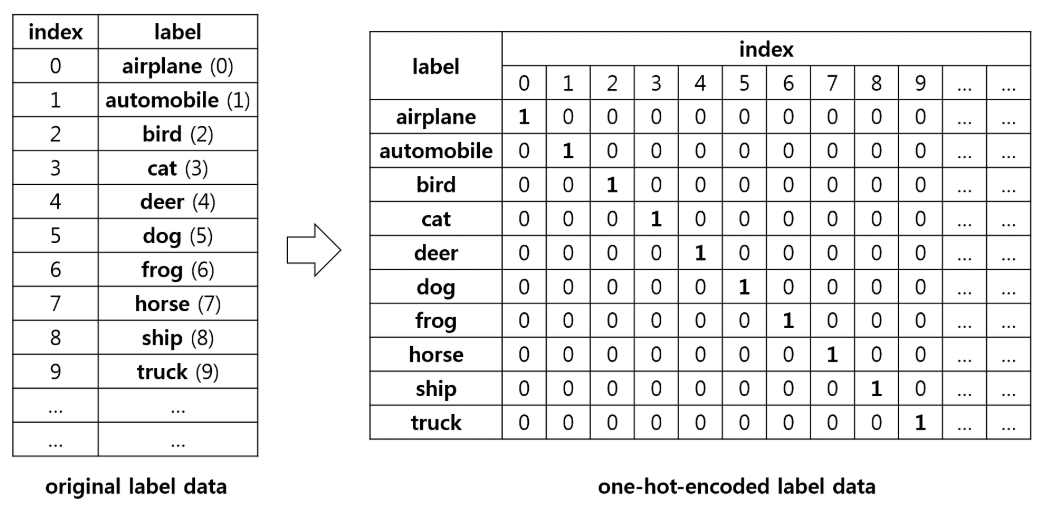
\includegraphics[scale=0.55]{figures/ohe-cifar10.png}
  \caption{One hot encoding of CIFAR-10 dataset. To the left, the categorical data label encoding. To the right, the one hot encoding.}
  \label{fig:ohe-CIFAR10}
\end{figure}

\subsubsection{Creating the CNN}

The CNN is created using keras library from Python. Its architecture is based on the classic CNN architecture illustrated on \autoref{fig:cnn-architecture} taking on input an image passing through convolutional layers and a fully connected layer giving the output class. Below is described the basic structure of our implemented CNN (baseline). \\

\textbf{Model basis}

When using keras, it allows two ways to generate a model: sequential or functional. The major difference between them is that the functional model allows you to connect layers to more than just the previous and next layers which allows you to create much more complex models and networks. In our case, it is not necessary. A sequential model is widely sufficient. Indeed, its limit is defined by its incapacity to share layers or have multiple inputs or outputs which is not necessary to resolve a simple image classification problem. The model is then created using the following method: 
\begin{center}
\texttt{Sequential()}
\end{center} 

\textbf{Convolutional layers}

Once the basis of the model has been created, we can generate the first convolutional layers. As we manage images, we have to use 2D convolutional layer which mainly take the number of filters for the convolution, the filter's size and the input shape as parameters. The keras method to create a 2D convolutional layer is then basically defined by:
\begin{center}
\texttt{Conv2D(filters, filter\_size, input\_shape)}
\end{center}
In our case, we use 32 as starting filters number which doubles each time we add a convolutional layer. The size of each filter is a 3x3 window. We also add \texttt{padding="same"} (which defines that we do not change the input image size) as well as its activation function as parameters. We generally use \texttt{ReLU} as activation function which is the most widely used activation function in neural networks today such as the AlexNet architecture. The exhaustive list of \texttt{Conv2D} method parameters can be found on the official keras library documentation \cite{keras-doc}. 

Between each layer, we use batch normalization which normalizes the inputs heading into the next layer using, ensuring that the network always creates activations with the same distribution that we desire \cite{CIFAR10-implementation-2}: 
\begin{center}
\texttt{BatchNormalization()}
\end{center}

After creating two convolutional layers, we generate a pooling layer of size 2x2 which compresses the information of the image to make it smaller (see \autoref{sec:pooling-layers} for full explanation). The pooling layer is created using: 
\begin{center}
\texttt{MaxPooling2D(size)}
\end{center}
It's important to not have too many pooling layers, as each pooling discards some data. Pooling too often will lead to a too small number of information that can be used for the next layers (densely connected layers) to learn about the data. Generally, we add a pooling layer between 2 convolutional layers to reduce the spatial volume of input image after convolution. 

Should we add another convolutional layer? There is no exact number of convolutional layers but each one added increases the number of filters so the model can learn more complex representations but obviously also adds more computation expenses. 

As we manage small sized images (32x32), the model that we are creating will be quite small. We then only add a third convolutional layer. Thus, we only pool once as our model contains only 3 convolutional layers. \\ 

\textbf{Fully-connected layer}

Before creating the fully-connected layer, we need to flatten the data to obtain the data into a 1-dimensional array (containing all the pixels data) for inputting it to the next layer so that he can process pixel by pixel to finally have the final output in the good format (a single vector of 10 elements representing the likelihood of each 10 outputs). We then add a flatten layer by using: 
\begin{center}
\texttt{Flatten()}
\end{center}

We can now create the fully-connected layer (dense layers) where the neurons have a complete connection to all the activations from the previous layers to generate a prediction from the results of these previous layers. A dense layer basically takes the number of neurons as parameter and then can be used in keras using (all parameters available in keras documentation \cite{keras-doc}:
\begin{center}
\texttt{Dense(neuronsNumber)}
\end{center}
The number of neurons chosen are starting from 256 which decreases in succeeding layers to finally approach the same number of neurons as there are classes in the dataset. Thus, we pass to the final layer the number of classes for the number of neurons (=10). Each neuron then represents a class with a certain probability that the image is belonging to this class. Moreover, as we want to prevent from overfitting, we also add a kernel constraint as parameter which regularize the data as it learns. 

Finally, as we have seen in \autoref{sec:fully-connected-layer}, we use \textit{Softmax} as activation function which selects the neuron with the highest probability as its output, voting that the image belongs to that class. 

The \autoref{fig:my-CNN} is summarizing the baseline of the CNN implemented. 

\begin{figure}[h]
  \centering
  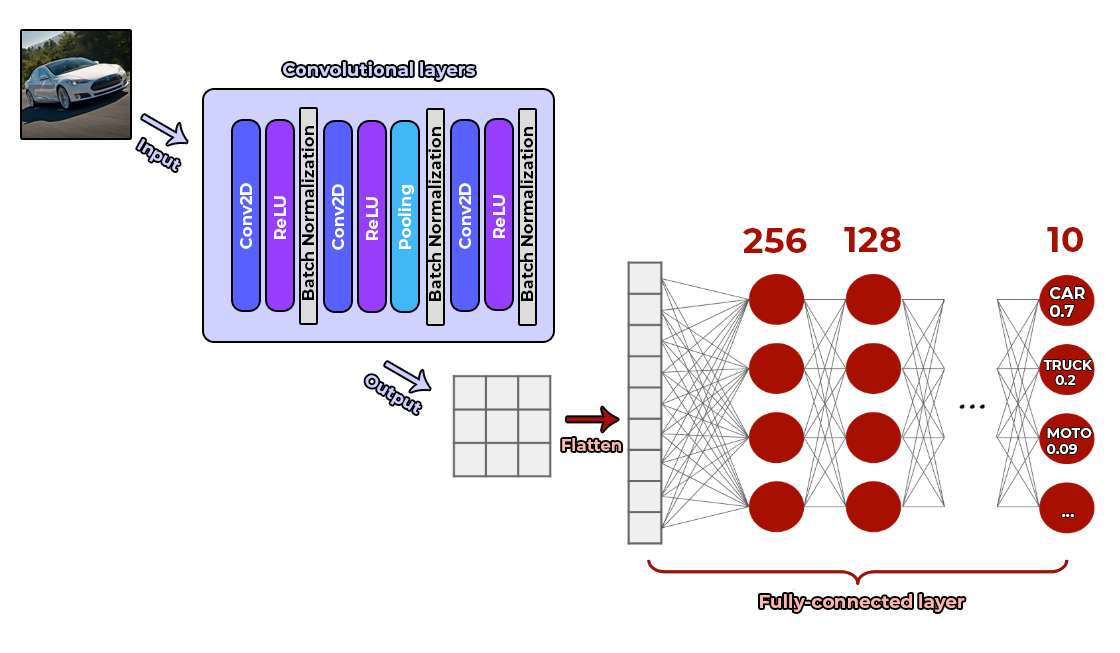
\includegraphics[scale=0.38]{figures/my-cnn.png}
  \caption{The baseline of the CNN implemented. In this example, the input image is a car and the CNN model outputs "car" as highest probability (0.7) and is then assigning the input image as "car" class.}
  \label{fig:my-CNN}
\end{figure}

\subsection{Summary pseudo-code}

\begin{algorithm}[H]
  \caption{Baseline CNN implementation} \label{alg:CNN}
  \begin{algorithmic}[1]
  \State Init the model: \texttt{Sequential()}
  \For {a number of convolutional layer to add}  
  \State Add convolutional layer
  \State ReLU activation function 
  \If {between 2 convolutional layer}
  \State Add pooling layer
  \EndIf
  \State Batch Normalization  
  \EndFor
  \State Flatten the data
  
  \For {a number of Dense layer to form the fully-connected layer}  
  \State Add dense layer
  \If {not last layer}
  \State ReLU activation function
  \State Batch Normalization 
  \Else 
  \State{Softmax activation function} 
  \EndIf
  \EndFor
  
  \State Compile the model 
  \State Train the model: \texttt{model.fit(X\_train, y\_train, X\_test, y\_test)} 
  \State Predict: \texttt{model.predict()}
  \end{algorithmic}
\end{algorithm}

\section{Optimizing parameters (Regularization)}
The CNN model created above is the simplest way to create a CNN and would probably not have the best prediction results. In this section, the different parameters that may enhance the accuracy and the results of our predictive CNN model are theoretically described in order to understand how to get better results. Generally, these parameters add information in order to prevent overfitting of which the process is called \textbf{regularization}.  

\subsection{Epochs}
When compiling your model, you give a number of epochs and a batch size to your model. Batch size may not influence the accuracy result but only the memory space needed. Higher the batch size, the more memory space you'll need. We usually use 64. In contrast, epochs certainly influences the performance of the model since an epoch refers to one cycle through the full training dataset. Thus, more epochs the model is learning, more features it will learn which can be damaging the model's performance due to overfitting, i.e. your model does not learn the data, it memorizes the data. Finding the good epochs number is then meaningful for the model's performance. 


\subsection{Optimizer}
Also at compilation step, you need to specify an optimizer. Optimizers are algorithms or methods used to change the attributes of your neural network such as weights and learning rate in order to reduce the losses. 

Optimizers algorithms are generally based on \textit{gradient descent algorithm} which is optimization algorithm used to minimize some function by iteratively moving in the direction of steepest descent as defined by the negative of the gradient \cite{gradient}. 

The choice of optimizers are based on the type of network, type of layers and type of data. In the \autoref{sec:exp-cnn}, we will experiment 5 different optimizers: RMSProp, ADAM, SGD, AdaGrad and AdaDelta. %p-e a expliquer 

\subsection{Dropout} \label{sec:dropout-cifar}
Dropout refers to ignoring units (i.e. neurons) during the training phase of certain set of neurons which is chosen at random. For instance, a dropout value of 0.2 means that you randomly select 20\% of the neurons and set their weights to zero for the forward and backward passes i.e. for one iteration. This dropout process is used to prevent from overfitting that can be led by neurons developing co-dependency amongst each other during training phase. 

\begin{figure}[h]
  \centering
  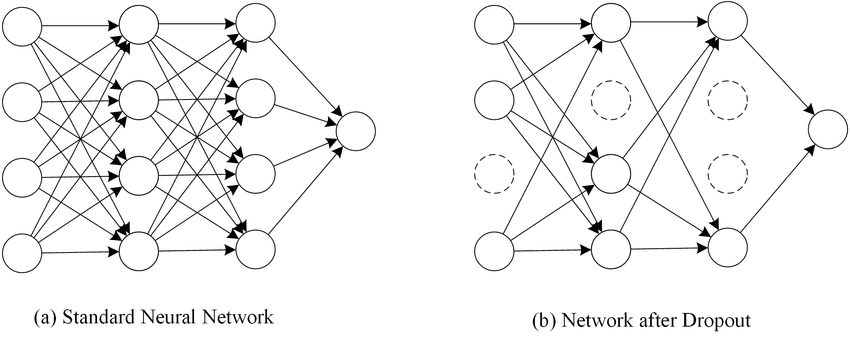
\includegraphics[scale=0.45]{figures/dropout.png}
  \caption{Dropout Neural Net Model. Left: A standard neural net with 2 hidden layers. Right: An example of a thinned net produced by applying dropout to the network on the left. Crossed units have been dropped. Figure extracted from \cite{dropout}}
  \label{fig:dropout}
\end{figure}

\newpage
\subsection{Weight decay}
Another way to prevent from overfitting is to use weight decay which involves updating the loss function to penalize the model in proportion to the size of the model weights. By updating weights this way, we penalize the learning complexity and then reduces the chance of overfitting. Weight decay is a regularization method existing by 3 types of regularizers, with $x$ a small number:
\begin{itemize}
\item $L1(x)$: we multiply the sum of the absolute weights with $x$.
\item $L2(x)$: we multiply the sum of the squared weights with $x$.
\item $L1L2(x)$: we multiply the sum of the absolute and squared weights with $x$.
\end{itemize}  
Generally, we use L2 weight regularization which is the most common type used for neural networks since L2 regularizer does not have sparse estimations and is computational efficient due to having analytical solutions. 


\subsection{Data augmentation}
Same as previous parameters, our objective is to reduce overfitting to generalizes well the data. Another way to allow the model to learn the same general features is making copies of the examples in the training dataset and add small random modifications to the images. It expands the dataset so that model learns to not take in account these modifications but only the general features. This process is called data augmentation. Many types of data application can be applied to images such as cropping, rotating, shifting, zooming, random erasing, etc.   

\begin{figure}[H]
  \centering
  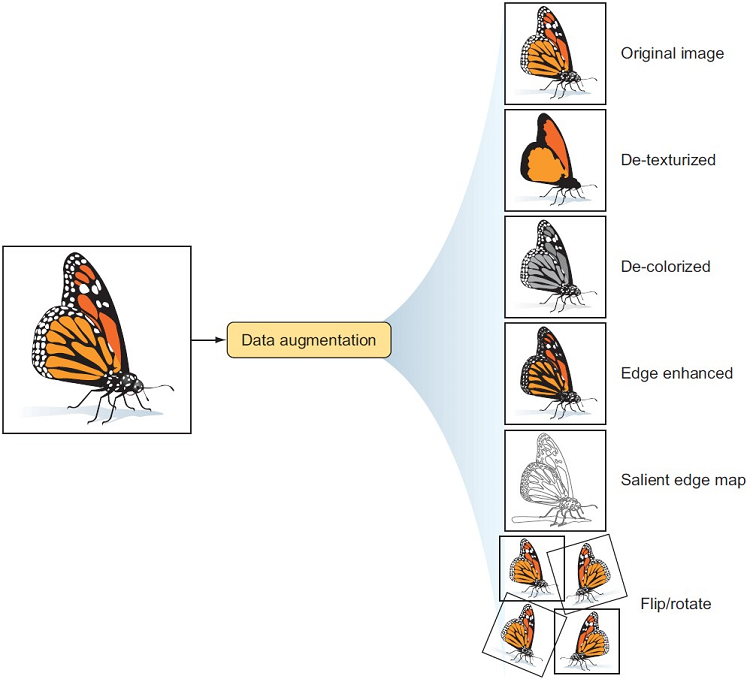
\includegraphics[scale=0.55]{figures/data_augmentation.png}
  \caption{Some image data augmentation examples. Figure extracted from \cite{data-aug-examples}}
  \label{fig:dropout}
\end{figure}


\subsection{Adding noise} \label{sec:noise-cifar}
% https://www.researchgate.net/figure/Performance-on-CIFAR-10-for-varying-amounts-of-noisy-labels-Noisy-training-examples-are_fig2_317241165 
% https://machinelearningmastery.com/how-to-improve-deep-learning-model-robustness-by-adding-noise/ 
What if the images are getting noisy over time? Is the model reacting well to that kind of perturbations? Theoretically, if the model suffers from overfitting, adding noise may be benefit to the accuracy of the model for the reason that learning noisy images is more complex and the model may only distinguish general features and big lines of the images.
Thus, adding noise during the training phase should have a regularization effect and can make the training process more robust and reduce generalization error. 

The most common type of noise is Gaussian noise illustrated in \autoref{fig:gaussian-noise}. Of course, adding noise is done relating to a configurable hyperparameter. The choice of this value is then decisive since too little noise has no effect, whereas too much noise makes the mapping function too challenging to learn. 

\begin{figure}[h]
  \centering
  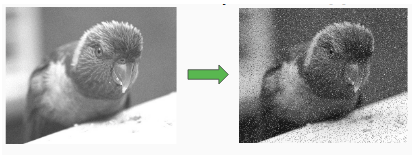
\includegraphics[scale=1]{figures/gaussian-noise.png}
  \caption{Illustration of adding Gaussian noise to an image. The image becomes blurry.}
  \label{fig:gaussian-noise}
\end{figure}

 

\section{Experiments and results}

Several experiments testing the efficiency of the different parameters are done and the corresponding results are presented to find optimal parameters. 

\subsection{Experiments} \label{sec:exp-cnn}
Here under are the experiments that have been done in order to encompass all the parameters tests to show how the CNN model react to them and how they impact its performance. So that, each parameter are approached \textbf{separately} (= without any other regularizer than the parameter in question). These experiments are done with sampling on 1 batch of the training set (10000 images) on 5 epochs. Note that the sampling is \textbf{not stratified} which means that the batch selected does not respect the proportions of each class from the complete dataset. Moreover, we also have done the experiments concerning regularizers (experiment 3 to 6) on the complete training set also on 5 epochs. Indeed, regularizers are processes used to counter overfitting. Therefore, using the whole training set may be more reliable to observe their efficiency. For both cases, the testing phase has been done on the test set (10000 images). They all have been done using AdaDelta as optimizer (except experiment 2 obviously). 

\begin{itemize}
\item \textit{Experiment 1 - Epochs number:} run on 40 epochs, on the baseline CNN without any regularizer (= no dropout, no weight decay, no data augmentation and no added noise) 

\item \textit{Experiment 2 - Optimizer:} 5 runs testing the following optimizers: RMSProp, ADAM, SGD, AdaGrad and AdaDelta. 

\item \textit{Experiment 3 - Dropout value:} 6 runs with the following dropout values: 
\newline $[0, 0.1, 0.2, 0.4]$, the last value means that the dropout value is increasing from 0.2 to 0.5 over layers.
 
\item \textit{Experiment 4 - Weight decay values:} 2 runs with the following weight decay values: $[0.001, 0.01]$.   

\item \textit{Experiment 5 - Data augmentation:} unique run with data augmentation on images : horizontal flip, minor shifts of the image and small zooming.

\item \textit{Experiment 6 - Adding Gaussian noise:} 3 runs with the following Gaussian noise rate: $[0.1, 0.2, 0.4]$.
\end{itemize}

\subsection{Results} 

\textit{N.B.: As we use sampling to avoid multiple large execution times, the results may be quite lower compared to if we have used the whole dataset. Nevertheless, these results can be more significant since the training set is highly imbalanced.}    

\subsubsection{Experiment 1 - Epochs number} 
What we can see from the results presented in \autoref{fig:cifar_epoch_res} is that the accuracy reaches $\approx 100\%$ for the training set after only 5-6 epochs which shows that using more epochs should not be relevant and even counterproductive. Indeed, we can see that the global accuracy is not evolving and stalling around 65\% between 10 and 40 epochs which shows the uselessness of using too much epochs. 

\begin{figure}[H]
  \centering
  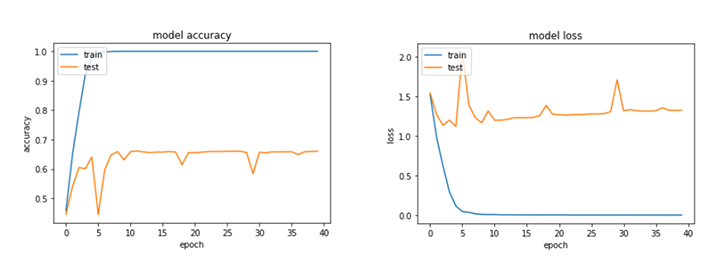
\includegraphics[scale=0.6]{Code/ch5-ModelPrototype/figures_result/40epochs_sample_withoutoptimisation.PNG}
  \caption{Experiment 1 result: model accuracy and lost over epochs.}
  \label{fig:cifar_epoch_res}
\end{figure}
 
\subsubsection{Experiment 2 - Optimizer} 

This experiment represents the results without any regularizer depending only on optimizer choice.

The general behaviour of the results observed about the optimizers is that SGD (Stochastic gradient descent) seems to not be a good optimizer in this case. Indeed, SGD is very basic and rarely used now: although SGD minimizes loss faster, it is noisier and it oscillates around the the minimum giving some variation in accuracy and loss run to run.

The other optimizers as for them have quite similar results even if ADAM and AdaGrad seems to be the most adapted in our case. In fact, their algorithm is quite similar too: RMSProp and AdaDelta have both been developed independently but AdaDelta is an extension of AdaGrad and ADAM is somehow a combination of AdaDelta and RMSProp. However, we generally use AdaGrad to deal with sparse data and ADAM for more general cases since it requires relatively low memory and combines the good properties of AdaDelta and RMSProp. That may explain why ADAM and AdaGrad stand out from the crowd. 

\begin{center}
\begin{tabular}{|c|c|}
  \hline
  Optimizer & Accuracy (with sampling) \\
  \hline
  RMSProp & 54.640\% \\
  ADAM  & 61.220\% \\
  SGD & 51.720\% \\
  AdaGrad & \textbf{63.490\%} \\
  AdaDelta & 55.770\% \\
  \hline
\end{tabular}
\captionof{table}{Experiment 2 results.}  
\end{center}


\subsubsection{Experiment 3 - Dropout value} 

For the sampling case, we see that the best result is obtained while not using dropout. It is somehow logical since sampling removes already lot of information and is hence less subject to overfitting but more to underfitting. 

However, when using the entire training set, it is more to be prone to overfitting. That is why we obtain better results when using dropout. Watch out, we have to take care of the value of dropout added. Indeed, the results show that see that a too high dropout value is decreasing drastically the accuracy which means that too much dropout was done impacting the capacity of the model to learn well. On the following results, we see that a dropout value above 0.2 is decreasing the accuracy which can be considered as the threshold value which impact negatively the model's learning. Using keras, dropout can be added using \texttt{model.add(Dropout(dropoutValue))}. 

\begin{center}
\begin{tabular}{|c|c|c|}
  \hline
  Dropout value & Accuracy (no sampling) & Accuracy (with sampling) \\
  \hline
  0 & 76.13\% &  \textbf{63.490\%} \\
  0.1 & 76.51\% & 55.530\% \\
  0.2 & \textbf{78.140\%} & 57.840\% \\
  0.4 & 59.890\% & 45.140\% \\
  \hline
\end{tabular}
\captionof{table}{Experiment 3 results table.}  
\end{center}


\begin{figure}[H]
  \centering
  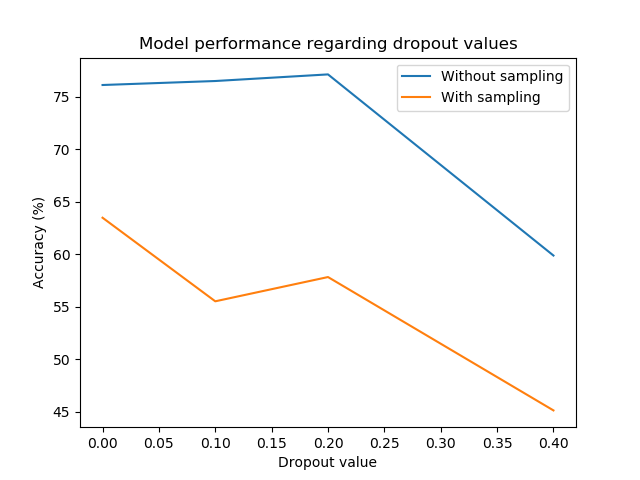
\includegraphics[scale=0.6]{Code/ch5-ModelPrototype/figures_result/dropout_graph.png}
  \caption{Experiment 3 result graph: the blue line is the experiment without sampling and the orange line is the one with sampling. $0.2 \rightarrow 0.5$ refers to the experiment using increasing dropout values.}
  \label{fig:cifar_dropout_res}
\end{figure}

\subsubsection{Experiment 4 - Weight decay values} 

The impact of weight decay looks a bit less effective as dropout in most and general cases. But in the sampling case, we now observe a small accuracy enhancement which was not observable when using dropout. However, using larger weighting (0.01) looks to not be a good idea neither since weight decay is usually used with a very small weighting number. Using keras, weight decay is done by adding \texttt{kernel\_regularizer=l2(0.01)} to \texttt{Conv2D} parameters. 

\begin{center}
\begin{tabular}{|c|c|c|}
  \hline
  Weight decay value & Accuracy (no sampling) & Accuracy (with sampling) \\
  \hline
  0 & 76.13\% &  63.490\% \\
  0.001 & \textbf{77.470\%} & \textbf{64.190\%} \\
  0.01 & 76.090\% & 60.140\% \\
  \hline
\end{tabular}
\captionof{table}{Experiment 4 results table.}  
\end{center}

\begin{figure}[H]
  \centering
  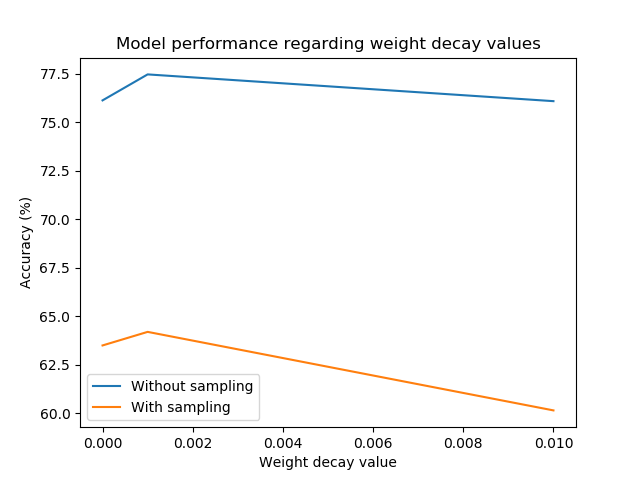
\includegraphics[scale=0.6]{Code/ch5-ModelPrototype/figures_result/weight_decay_graph.png}
  \caption{Experiment 4 result: the blue line is the experiment without sampling and the orange line is the one with sampling.}
  \label{fig:cifar_weightdecay_res}
\end{figure}


\subsubsection{Experiment 5 - Data augmentation} 

In both cases, we see an improvement compared to the baseline results. Data augmentation seems then to be a good process to enhance the model's accuracy. Making copies of the images with random modifications expands the training set passed to the model and then can only be benefit the model's learning. To implement data augmentation, we have used \texttt{ImageDataGenerator} method also from keras library.   

\begin{center}
\begin{tabular}{|c|c|c|}
  \hline
  Data augmentation & Accuracy (no sampling) & Accuracy (with sampling) \\
  \hline
  No & 76.13\% & 63.490\% \\
  Yes & \textbf{78.410\%} & \textbf{64.810\%} \\
  \hline
\end{tabular}
\captionof{table}{Experiment 5 results table.}  
\end{center}

\subsubsection{Experiment 6 - Adding Gaussian noise} \label{sec:noise-CIFAR10}
Same as previous regularizers, choosing the right added noise rate is really important. As the training set is highly balanced, this can be well observed in the non-sampling case where we observe that the accuracy is decreasing a lot when adding too much noise. This can easily be explained same as experiment 3 with dropout, i.e. in the sampling case, we learn less then we already have missing information (underfitting), adding noise is then not benefit to increase the model accuracy.

However, for the non-sampling case that the model is reacting well to noise since that the accuracy is not fluctuating at all and keep constant. This Gaussian noise has been added after the pooling layer by using \texttt{GaussianNoise(value)} from keras.   

\begin{figure}[H]
  \centering
  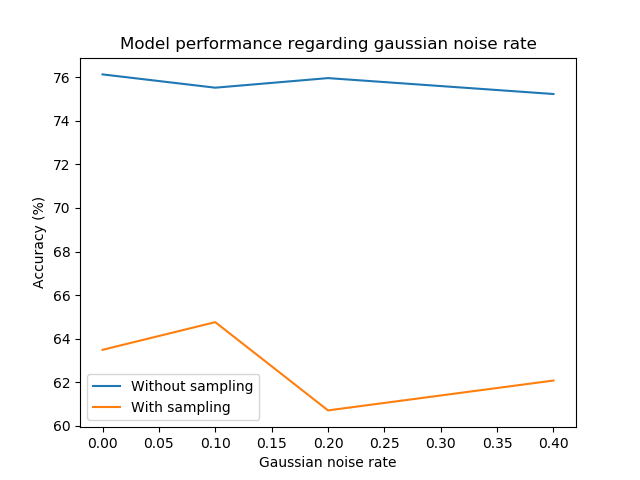
\includegraphics[scale=0.6]{Code/ch5-ModelPrototype/figures_result/gaussian_noise_graph.png}
  \caption{Experiment 6 result: the blue line is the experiment without sampling and the orange line is the one with sampling.}
  \label{fig:cifar_noise_res}
\end{figure}


\subsection{Conclusion}
When talking about image classification, the most popular model is a convolutional neural network. After creating a baseline CNN, several regularizers have been introduced and have been experimented to observe their impact on our model's accuracy. Following the results obtained, dropout regularizer and data augmentation seems to be the most efficient ones. After discussing about a simple non-medical case, we can henceforth tackle medical images using our knowledge about CNNs. 


\chapter{Identification of Leukemia Subtypes from microscopic images}

Leukemia is a malignant progressive disease that results in high numbers of abnormal blood cells in the bone marrow and other blood-forming organs. These abnormal blood cells suppress the production of normal blood cells leading to multiple symptoms. The main method to detect these abnormal blood cells is from microscopic images of blood's content. Moreover, leukemia is subdivided into a variety of large group which can also be detected by these microscopic images. In this chapter, we first tackle the detection of leukemia as a binary classification (ill/healthy) using the ALL-IDB dataset \cite{ALL-IDB}. In a second step, the different types of leukemia make object of a multi-class image classification problem. Experiments on these different types of leukemia will use the DEMIR-LEUKEMIA dataset \cite{leukemia}. This allows us to distinguish the difference between medical and non-medical images previously studied (CIFAR10). Are the methods the same? Are the regularizers used for non-medical images relevant for the medical ones? This chapter is based on the work of Ahmed et al \cite{leukemia}. 


\section{Subtypes of leukemia}
The two main subdivisions of leukemia are acute and chronic forms and can be defined following the National Cancer Institute: 
\begin{itemize}
\item \textbf{Acute} leukemia: A rapidly progressing cancer that starts in blood-forming tissue such as the bone marrow, and causes large numbers of white blood cells to be produced and enter the blood stream\cite{NCI}. Acute leukemia is then characterized by a rapid increase in the number of immature blood cells and needs to treated quickly since the cancer can evolve quickly. 
\item \textbf{Chronic} leukemia: A slowly progressing cancer that starts in blood-forming tissues such as the bone marrow, and causes large numbers of white blood cells to be produced and enter the blood stream \cite{NCI}. Chronic leukemia typically takes months or years to progress, the cells are produced at a much higher rate than normal, resulting in many abnormal white blood cells and is generally not diagnosed until symptoms, such as enlarged lymph nodes, appear.
\end{itemize} 

Acute and chronic leukemia can be subdivided into 2 more classes regarding which kind of blood cells is affected. These 2 classes are called lymphocitic and myelogenous leukemias. 

\begin{itemize}
\item \textbf{Lymphocitic} leukemia: A type of cancer in which the bone marrow makes too many lymphocytes (white blood cells) \cite{NCI}. 
\item \textbf{Myelogenous} leukemia: the cancerous change takes place in a type of marrow cell that normally goes on to form red blood cells, some other types of white cells, and platelets \cite{wiki-leukemia}. 
\end{itemize} 

There exists many more specific leukemia types but we will only approach these 4 main subtypes in the context of this document. These 4 subtypes of leukemia are summed up on \autoref{table:leukemia-subtypes} and illustrated by \autoref{fig:leukemia-subtypes}. 
We can see the importance of determining the leukemia subtype of the patient. A chronic leukemia is not as urgent as an acute leukemia that needs to be treated as soon as possible. 

\begin{center}
    \begin{tabular}{|c|c|c|}
      \hline
      Cell type & Acute & Chronic \\
      \hline
      Lymphocitic & Acute Lymphocitic Leukemia (\textbf{ALL}) & Chronic Lymphocitic Leukemia (\textbf{CLL})  \\
      \hline
      Myelogenous & Acute Myelogenous Leukemia (\textbf{AML})  & Chronic Myelogenous Leukemia (\textbf{CML})  \\
      \hline
    \end{tabular}
    \captionof{table}{Summary of the 4 main leukemia subtypes tackled in the document.}
    \label{table:leukemia-subtypes}
\end{center}

\begin{figure}[H]
  \centering
  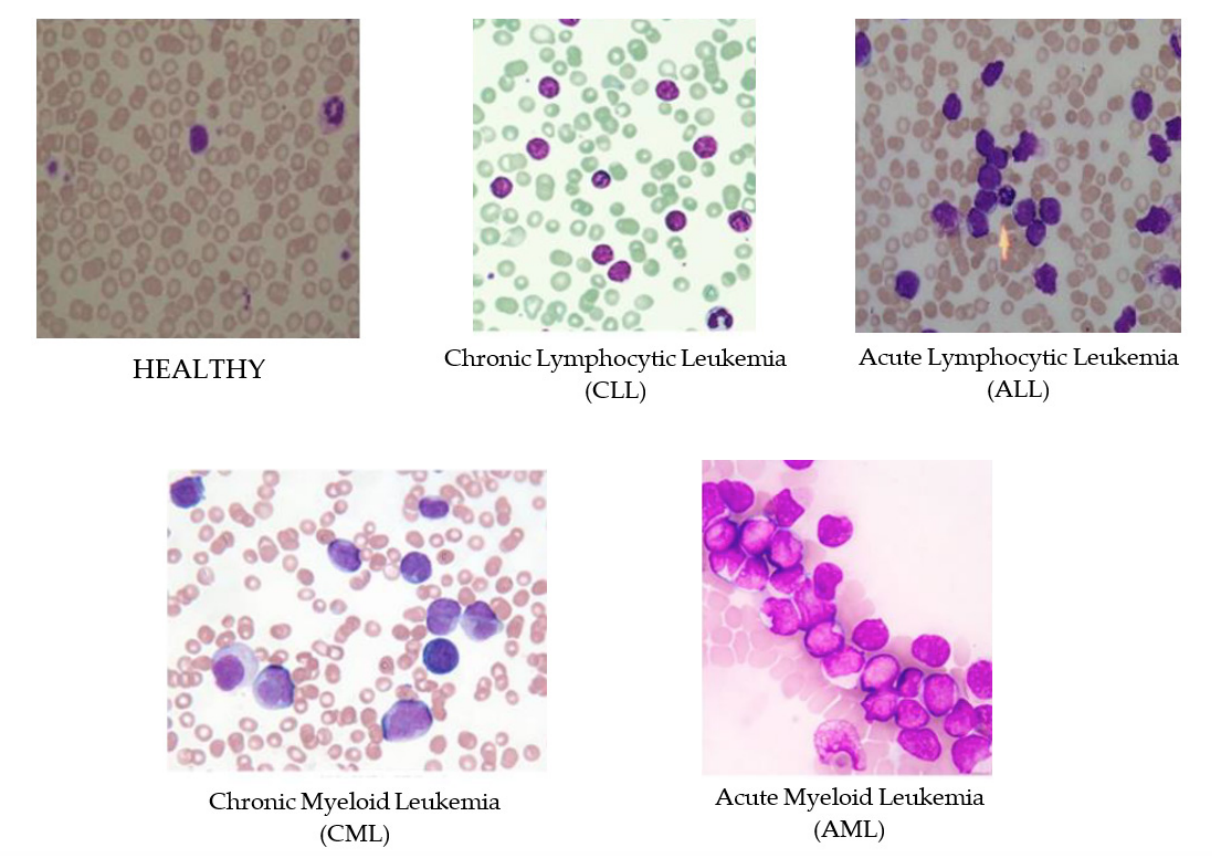
\includegraphics[scale=0.6]{figures/leukemia-subtypes.png}
  \caption{Sample images of four different types of Leukemia. From left to right, HEALTHY, Chronic Lymphocytic Leukemia (CLL), Acute Lymphocytic Leukemia (ALL), Chronic Myeloid Leukemia (CML), Acute Myeloid Leukemia (AML). Figure extracted from \cite{leukemia}}
  \label{fig:leukemia-subtypes}
\end{figure}

\newpage
\section{ALL-IDB dataset} \label{sec:all-idb}
The ALL-IDB dataset, fully named \textit{Acute Lymphoblastic Leukemia Image Database for Image Processing}, is provided by Fabio Scotti from the University of Milan \cite{ALL-IDB}. As its name indicates, the ALL-IDB dataset only contains microscopic images from patients that have the ALL type of leukemia when labelled positive to illness. For each image in the dataset, the classification/position of ALL lymphoblasts is provided by expert oncologists. 

The ALL-IDB dataset is divided into 2 sets of data: ALL-IDB1 and ALL-IDB2. 
\begin{itemize}
\item ALL-IDB1 contains large images of average size 2592 x 1944 which contains about 39000 blood elements spread into 108 images collected in September 2015. In these 108 images, 50 are labelled positive to leukemia and 58 labelled healthy. The ALL-IDB1 image files are named with the notation ImXXX\_Y.jpg where XXX is a 3-digit integer counter and Y is a boolean digit equal to 0 is no blast cells are present (healthy), and equal to 1 if at least one blast cell is present in the image (ill). As the images are large, ALL-IDB1 is quite useful for testing different image preprocessing methods such as segmentation or data augmentation to see their efficiency in the final classification accuracy.  As the dataset also provides the position of the blast cells in the image, this information may be used to estimate the location of the centroids of the blast cells as well as the number of ALL blast.  

\item ALL-IDB2 is a collection of cropped area of interest of normal and blast cells that belongs to the ALL-IDB1 dataset. These images are then somehow already preprocessed regarding the region of interest. Their size is $\approx$ 250 x 250. ALL-IDB2 images have similar gray level properties to the images of the ALL-IDB1, except the image dimensions. The images are annotated similarly to the images from ALL-IDB1. ALL-IDB2 contains 260 images including 130 ALL cases and 130 healthy cases.  
\end{itemize}


\begin{figure}[H]
  \centering
  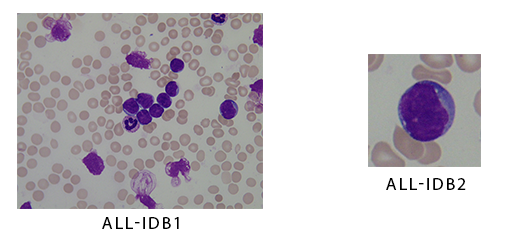
\includegraphics[scale=1]{figures/all-idb.PNG}
  \caption{Image examples of ALL-IDB1 and ALL-IDB2.}
  \label{fig:all-idb}
\end{figure}

\newpage
\section{DEMIR-LEUKEMIA dataset} \label{sec:demir-leukemia}
The DEMIR-LEUKEMIA dataset has been created by Ahmed et al. \cite{leukemia} from the The American Society of Hematology (ASH) Image Bank \cite{ASH}. Since ALL-IDB only deals with ALL leukemia subtype, the DEMIR-LEUKEMIA dataset is complementary to ALL-IDB by providing a collection of CLL, AML and CML leukemia subtypes images.  

ASH Image Bank is publicly available on the Web and includes a comprehensive collection of
images related to a wide range of hematological topics. In this study, Ahmed et al. have selected all available blood cell images annotated with leukemia, including any of CLL, AML and CML subtypes. 

DEMIR-LEUKEMIA contains 177 AML, 185 CLL and 185 CML images. It contains no healthy cases. The sizes of the images are very variables, it can goes from 200 x 200 to 1000 x 1000. As Ahmed et al. have chosen the images with no specific criteria except the leukemia subtype, the images are very disparate. When using this dataset, the preprocessing step is then mandatory. 

\autoref{table:datasets-leukemia} sums up the content of the two original datasets used for leukemia subtypes detection, i.e. the number of samples. 

\begin{center}
    \begin{tabular}{|c|c|c|c|c|c|c|}
      \hline
      \textbf{Dataset} & \textbf{ALL} & \textbf{AML} & \textbf{CLL} & \textbf{CML} & \textbf{HEALTHY} & \textbf{Total}\\
      \hline
      ALL-IDB1 & 50 & 0 & 0 & 0 & 58 & 108  \\
      \hline
      ALL-IDB2 & 130 & 0 & 0 & 0 & 130 & 260  \\
      \hline
      ALL-IDB & 180 & 0 & 0 & 0 & 188 & 368  \\
      \hline
      DEMIR-LEUKEMIA & 0 & 177 & 185 & 185 & 0 & 547  \\
      \hline
      \hline
      ALL-IDB + DEMIR-L & 180 & 177 & 185 & 185 & 188 & 915 \\ 
      \hline
    \end{tabular}
    \captionof{table}{Summary of the ALL-IDB and DEMIR-LEUKEMIA datasets used for leukemia subtypes detection.}
    \label{table:datasets-leukemia}
\end{center} 

\section{Data augmentation on datasets} \label{sec:data-aug-leuk}

In addition to the original datasets, these data have also been augmented using multiple minor images transformations in order to have larger datasets. Data augmentation techniques were widely utilized to increase the dataset size and avoid memorization. As the images change and the pixels are moved, the neural network would think these are distinct. The transformations that have been applied are listed below: 

\begin{itemize}
\item \textbf{Rotation}: random rotations between -25° (left rotation) and 25° (right rotation). The rotation effect has usually good impact on the neural network as the change is very minor and then the features impacting the label can also be recognized as the original. Nevertheless, the corners of the images are black due to the rotation that can negatively impact the learning of the neural network especially if we manage small images. Indeed, the black area can dominate the image and can be considered as an important feature to determine the label. This rotation has been done using the \texttt{sk.transform.rotate()} method from \texttt{skimage} library in Python.  
  
\item \textbf{Horizontal flip}: reverse the image horizontally, the image generated is a mirror-reversal of an original across a horizontal axis image. Pixels were moved horizontally from one half of the image to the other half. In contrary to simple rotation, flipping the image does not imply black areas and is then theoretically beneficial to the learning.    

\item \textbf{Vertical flip}: reverse the image vertically, the image generated is a mirror-reversal of an original across a vertical axis image. Pixels were moved vertically from one half of the image to the other half.

\item \textbf{Noise}: random noise added to the image. As seen in the previous experiments done on the CIFAR10 dataset (see \autoref{sec:noise-CIFAR10}), gaussian noise has relatively a good regularizer impact on the network. We then use the assumption that it would also have a positive impact on medical images. This noise has been added using the \texttt{sk.util.random\_noise()} method from \texttt{skimage} library in Python.   

\item \textbf{Uniform filter}: similarly as noise, the uniform filter that we apply there is to reduce the sharpness of the image, i.e. the image is somehow blurred and can easily be compared as noise. This uniform filter has been added using the \texttt{ndimage.uniform\_filter()} method from \texttt{scipy} library in Python.   

\item \textbf{Random gamma}: gamma defines the relationship between a pixel's numerical value and its actual luminance. In other words, gamma impacts the contrast and the luminosity of the image. In this study, modifying the gamma could be a reliable transformation to detect features as the edges of the shapes can be made more visible. This uniform filter has been done using the \texttt{exposure.adjust\_gamma()} method from \texttt{skimage} library in Python.    
\end{itemize} 

All these transformations are illustrated by order in \autoref{fig:data_augmentation_leuk}.

When using data augmentation, people are also usually applying shifts and crops to their images. Here, I decided to not use these two as shifting or cropping an image is more likely affected by information loss and could be then not relevant for the model's enhancement. 

\begin{figure}[H]
  \centering
  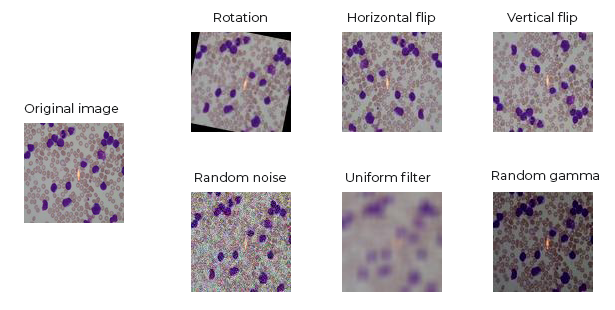
\includegraphics[scale=0.7]{figures/data_augmentation_leuk.PNG}
  \caption{Image transformations used for data augmentation. From left to right: original, rotation, horizontal flip, vertical flip, random noise, uniform filter and random gamma.}
  \label{fig:data_augmentation_leuk}
\end{figure}

% expectation : good but prolly bad car les images se ressemblent assez et le sens des images pourraient être une feature impactant 

\newpage

To create the transformed dataset, we apply randomly one of the transformations described above to each image from the original dataset. Each image has been augmented, thus we obtain a stratified dataset where the proportion of each label is not impacted and is similar to the original dataset. In that case, as we are creating one "copy" of each image, we are doubling the dataset size, then the number of images assigned to each label is also doubled. (e.g. if we have 2 classes of 40 "healthy" and 30 "ill", after data augmentation, we obtain 80 "healthy" and 60 "ill")

All the datasets with their corresponding number of images per leukemia subtypes are summarized in \autoref{table:datasets-leukemia-final}. 

\begin{center}
    \begin{tabular}{|c|c|c|c|c|c|c|}
      \hline
      \textbf{Dataset} & \textbf{ALL} & \textbf{AML} & \textbf{CLL} & \textbf{CML} & \textbf{HEALTHY} & \textbf{Total}\\
      \hline
      ALL-IDB1 & 50 & 0 & 0 & 0 & 58 & 108  \\
      \hline
      ALL-IDB1 (+ data aug.) & 100 & 0 & 0 & 0 & 116 & 216  \\
      \hline
      ALL-IDB2 & 130 & 0 & 0 & 0 & 130 & 260  \\
      \hline
      ALL-IDB2 (+ data aug.) & 260 & 0 & 0 & 0 & 260 & 520  \\
      \hline
      ALL-IDB & 180 & 0 & 0 & 0 & 188 & 368  \\
      \hline
      ALL-IDB (+ data aug.) & 360 & 0 & 0 & 0 & 376 & 736  \\
      \hline
      DEMIR-LEUKEMIA & 0 & 177 & 185 & 185 & 0 & 547  \\
      \hline
      DEMIR-LEUKEMIA (+ data aug.) & 0 & 354 & 370 & 370 & 0 & 1094  \\
      \hline
      \hline
      ALL-IDB + DEMIR-L & 180 & 177 & 185 & 185 & 188 & 915 \\ 
      \hline
      ALL-IDB + DEMIR-L (+ data aug.) & 360 & 354 & 370 & 370 & 376 & 1830 \\ 
      \hline
    \end{tabular}
    \captionof{table}{Summary of the ALL-IDB and DEMIR-LEUKEMIA datasets used for leukemia subtypes detection in addition with data augmentation datasets.}
    \label{table:datasets-leukemia-final}
\end{center} 

\section{Methodology}

The methodology used is based on the article "Identification of Leukemia Subtypes from
Microscopic Images Using Convolutional Neural Network" from Ahmed et al. \citep{leukemia}. As the article's statement indicates, the model used is a convolutional neural network and can easily be justified (cfr. \autoref{sec:why-cnn}). 


\subsection{Preprocessing}
In the article \cite{leukemia}, no preprocessing phase was done to the images and are used from their original sizes and colors. In average, the images from the datasets used are quite large ($\approx$ 1500x1000) and requires a huge processing time if used at this size from a classic student laptop. Because of that, a preprocessing step is mandatory to avoid endless execution. In this case, the preprocessing is defined by: 
\begin{itemize}
\item Resize of all the images of a fixed size 100x100, illustrated in \autoref{fig:preproc-leuk} (a). 
\item In some experiments, we have applied some filters before processing the images: images to \textbf{greyscale}, images' \textbf{contrast increased} by an arbitrary value, \textbf{histogram equalization} of the images which is a method of contrast enhancement. This method consists on spreading out the most frequent intensity to make lower local contrast to gain a higher contrast. The principle of histogram equalization is illustrated in \autoref{fig:hist-eq}. A variant of histogram equalization (CLAHE) has been has been used and explained in \autoref{sec:img-enhancement-breast}. These filters have as objective to enhance the images by highlighting the important features of the images.  
\end{itemize}

\begin{figure}[H]
  \centering
  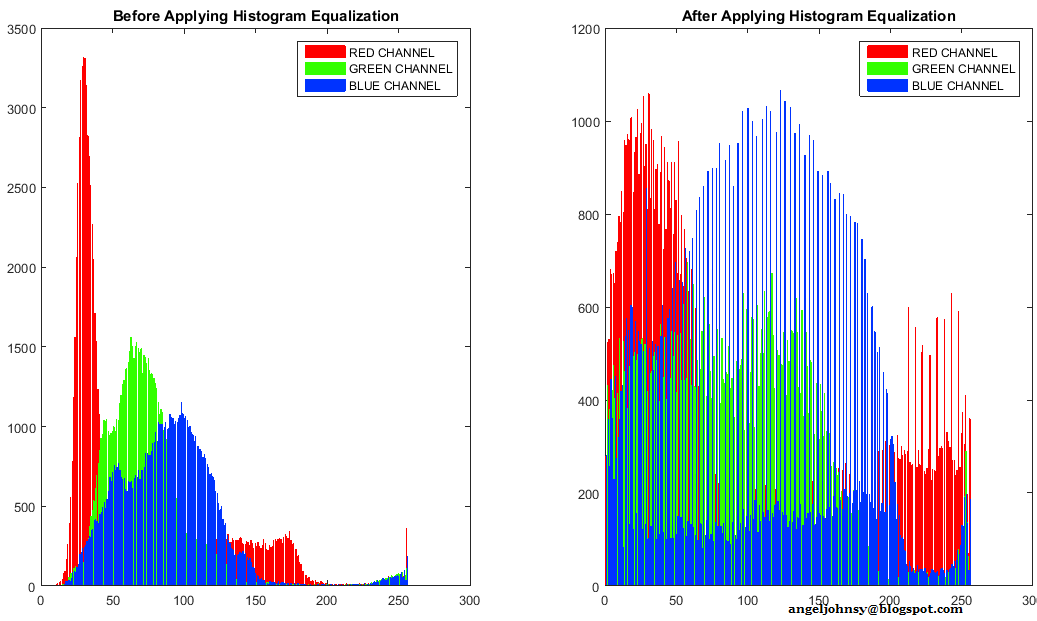
\includegraphics[scale=0.3]{figures/color_histogram_plot.png}
  \caption{Histogram equalization principle. A color histogram of an image represents the number of pixels in each type of color component. We spread out the most frequent intensity values of each color channel. Image extracted from \cite{hist-eq-fig}.}
  \label{fig:hist-eq}
\end{figure}

These preprocessing steps are illustrated in \autoref{fig:preproc-leuk}. 

Moreover, multiple questions are raised from this preprocessing: 

\begin{itemize}
\item Are informations still available from very small images? What is the capacity of the neural network to find the information? 
\item What informations are reliable to the training of a neural network? Is color needed to enhance the training? Is the direction of the images an impacting feature, i.e. are rotations and flips really relevant in this type of images?  
\item What is the best filter to apply on medical images? Which filter facilitates the model to retrieve the information on such images? 
\item Despite the preprocessing applied, can we still obtain good prediction rate? 
\end{itemize} 

\begin{figure}[H]
  \centering
  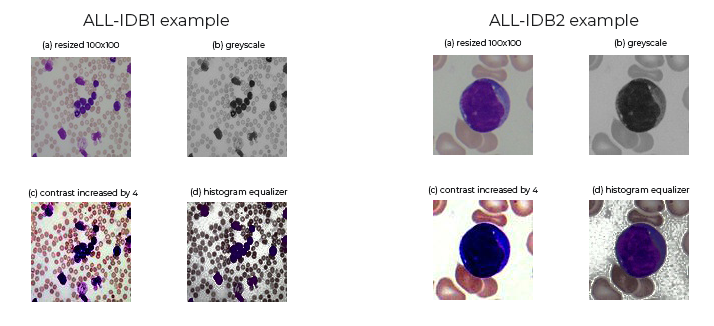
\includegraphics[scale=0.5]{figures/preproc-leuk.PNG}
  \caption{Example of preprocessing to an image of the dataset ALL-IDB1 and ALL-IDB2. (a) Image resized to 100x100 pixels, (b) grey-scale applied to the resized image, (c) image contrast increased, (d) histogram equalization applied.}
  \label{fig:preproc-leuk}
\end{figure}

\newpage
\subsection{CNN architecture}
As reminder, CNN is composed of convolution layers, pooling layers, flattening, and
multilayer perceptron. The number of layers and its respective parameters are chosen based on our previous study on CIFAR10 dataset done in \autoref{sec:CIFAR10-exp} and the article cited above \cite{leukemia}. Here below are described the choices done in the further experiments: 

\begin{itemize}
\item \textbf{Convolutional layers:} only 2 convolutional layers as the images are very small, 32 and 64 filters of size 3x3 with ReLU as activation function.  

\item \textbf{Max-Pooling layers:} one pooling layer after each convolutional layer (then total of two) of size 2x2. 

\item \textbf{Flatten layer:} one flatten layer between the convolutional layers and the fully-connected layer to transform the 2-dimensional max-pooled matrix into one dimensional array used as input for the fully-connected layer. 

\item \textbf{Fully-connected layer:} composed of two hidden layers (dense layers) and an output layer. The two hidden layers are respectively composed of 128 neurons and 64 neurons. The output layer contains as much as neurons than possible outputs.  
\end{itemize}

$\rightarrow$ Each layer is followed by a Batch normalization. 


\section{Experiments and results}

The following experiments are mainly based on the experiments done by Ahmed et al in their article \cite{leukemia}. However, some additional experiments are done to understand better how the model reacts and what are the best configuration to learn and predict better. In addition to my own results, when similar experiments were done, the results obtained by the authors of this article are also taken over in order to compare them and see the impact of the preprocessing. 

\subsection{Experiments}

In this study, we have 3 different datasets available: ALL-IDB1, ALL-IDB2 - which contains ALL and HEALTHY cases (described in \autoref{sec:all-idb} and DEMIR-LEUKEMIA - which contains AML, CLL and CML cases (described in \autoref{sec:demir-leukemia}). Having these 3 datasets, experiments will be done separately divided in 3 cases: 

\begin{itemize}
\item \textit{Case A - ALL-IDB1:} in this case, we only manage a binary classification between the ALL and HEALTHY cases. The images are not segmented and groups multiples blood cells. 

\item \textit{Case B - ALL-IDB2:} the second set of ALL-IDB contains segmented blood cells images and allow us to determine the potential improvement of the learning thanks to the segmentation. The question that can be raised using ALL-IDB2 is: "Does it give enough information?". 

\item \textit{Case C - All datasets:} runs on set of all images available: ALL-IDB and DEMIR-LEUKEMIA. This case involves the 4 subtypes of leukemia and the HEALTHY case. There are then 5 classes. 
\end{itemize}   


The experiments are realised on 25 epochs and batch size of 32 with ADAM optimizer. These choices have been made by the authors of \cite{leukemia} after multiple experiments that have noticed that working with 25 epochs performs better than longer epoch periods. The test set is defined by 20\% of the complete dataset. Each experiment has been repeated 5 times, the training set and the test set always change at each repetition. Note that this is not a 5-fold cross-validation since the train/test sets split is done randomly. The choice of not using a 5-fold cross-validation is due to the format and the order of the dataset which contains first all the ALL cases then all the AML cases then all the CLL cases and finally the CML cases. Using cross-validation would therefore not have been reliable since the test set would only contain one class. 

\begin{itemize}
\item \textit{Experiment 1 - Baseline:} 5 runs on the resized images of size 100x100 in color using the baseline CNN: no dropout and no data augmentation.  

\item \textit{Experiment 2 - With filters:} runs on the resized images with filters applied (greyscale, contrast increased or histogram equalization) of size 100x100 using the baseline CNN: no dropout and no data augmentation. Each filter is tested separately in order to see the impact of each filter. 5 runs are then done for each filter which involves a total of 15 runs.

\item \textit{Experiment 3 - Size 200x200:} 5 runs with larger resized images of size 200x200 in color using the baseline CNN: no dropout and no data augmentation.   

\item \textit{Experiment 4 - Noise:} runs on the resized images of size 100x100 with different level of noise applied. The level of noise applied are respectively $[0.1, 0.2, 0.4, 0.6, 0.8]$. We use the baseline CNN.  Each noise level is ran 5 times. 25 runs are then done in total. 

\item \textit{Experiment 5 - Dropout:} 5 runs on the resized images of size 100x100 in color using dropout set to 0.1 with no data augmentation. 
 
\item \textit{Experiment 6 - Data augmentation:} 5 runs on the data augmented dataset (described in \autoref{sec:data-aug-leuk}) with no dropout.   

\item \textit{Experiment 7 - Dropout and data augmentation:} 5 runs on the data augmented dataset (described in \autoref{sec:data-aug-leuk}) using dropout set to 0.1. 


\end{itemize}


\section{Results}

In this section, the results of the experiments described in the previous section are presented. For each experiment, 3 results' graphs are presented: 

\begin{itemize}
\item \textit{the evolution of the \textbf{accuracy} on the \textbf{test set} along epochs:} the indicator of how often the classifier was correct. 
\item \textit{the evolution of the value of \textbf{cost function} on the \textbf{test set} along epochs:} the cost function quantifies the error between predicted values and expected values and presents it in the form of a single real number \cite{TDS-CostFunction}, i.e. measure of how wrong the model is in terms of its ability to estimate the relationship between X and y. In our case, we want the cost function to be minimized.  
\item \textit{the evolution of the \textbf{accuracy} on \textbf{train set} along epochs:} this graph is used to visualise the speed at which the model learns and converges to 100\% accuracy (convergence state). 
\end{itemize}

In each result graph, the result of each run is drawn as well as the average of the 5 runs highlighted. 

\subsection{Case A - ALL-IDB1}

For the first case, we use the ALL-IDB1 dataset which contains a total of 108 images. We then use 86 images for training and 22 images for testing when not using data augmentation. Otherwise, we have 172 images for training and 44 images for testing. As reminder, ALL-IDB1 dataset contains only 2 classes: HEALTHY (label 0) vs ILL (label 1) and contains a large view of blood cells of the patient. ALL-IDB dataset is explained in details in \autoref{sec:all-idb}.    

\subsubsection{Experiment A.1 - Baseline}

This experiment consists of trying the simplest version of the CNN and observe how it reacts to the resized original dataset. To make a general idea about the efficiency of our model, we can refer to the results obtained by Ahmed et al on his work \cite{leukemia}. They obtained an average of 81.16\% accuracy on test set, 1.3093 for loss value and 99.55\% for train set without applying any image transformations. 

Generally, the results obtained are not so far than the results obtained by the reference article \cite{leukemia} knowing that we have used images resized to 100x100 (= 10000 pixels). Thus, the images that we have used have \textbf{22 times less pixels} since the original images are sized of $\approx$ 1700x1300 (= 221000 pixels). 

We can certainly assure that this resizing impacts the performance of our CNN model and can cause some troubles in its capacity to learn and retrieve the information. Nevertheless, despite this huge inconvenience, the CNN is still capable of learning some features otherwise we would have an average accuracy of 50\% in this type of binary classification.   
We can observe that the CNN converges very quickly -- no more than 5 epochs, to its convergence state.  

The general behaviour when looking to the results graphs on \autoref{fig:results-A1} is that the accuracy tends to increase slowly and stabilize at a certain time. Same for the loss value, it tends to decrease along time.  

\vspace{1cm}


\begin{center}
\begin{tabular}{|l|c|c|c|c|c|c|}
  \hline
   & \textbf{Run 1} & \textbf{Run 2} & \textbf{Run 3} & \textbf{Run 4} & \textbf{Run 5} & \textbf{AVG}\\
  \hline
  ACC-TEST & 68.18\% & 63.63\% & 59.09\% & 63.63\% & 72.72\% & 65.45\% \\
  LOSS-TEST & 3.53 & 5.86 & 6.55 & 0.55  & 0.82 & 3.46 \\ 
  ACC-TRAIN & 100\% & 100\% & 100\% & 100\% & 100\% & 100\% \\ 
  \hline
\end{tabular}
\captionof{table}{Experiment A.1 (On ALL-IDB1, with Baseline) - Train set = 86 images, Test set = 22 images - Detailed results of each run after 25 epochs. ACC-TEST is the accuracy result on test set, LOSS-TEST the value of cost function on test set and ACC-TRAIN the accuracy result on train set.}
\label{table:results-A1}
\end{center}


\begin{figure}[H]
  \centering
  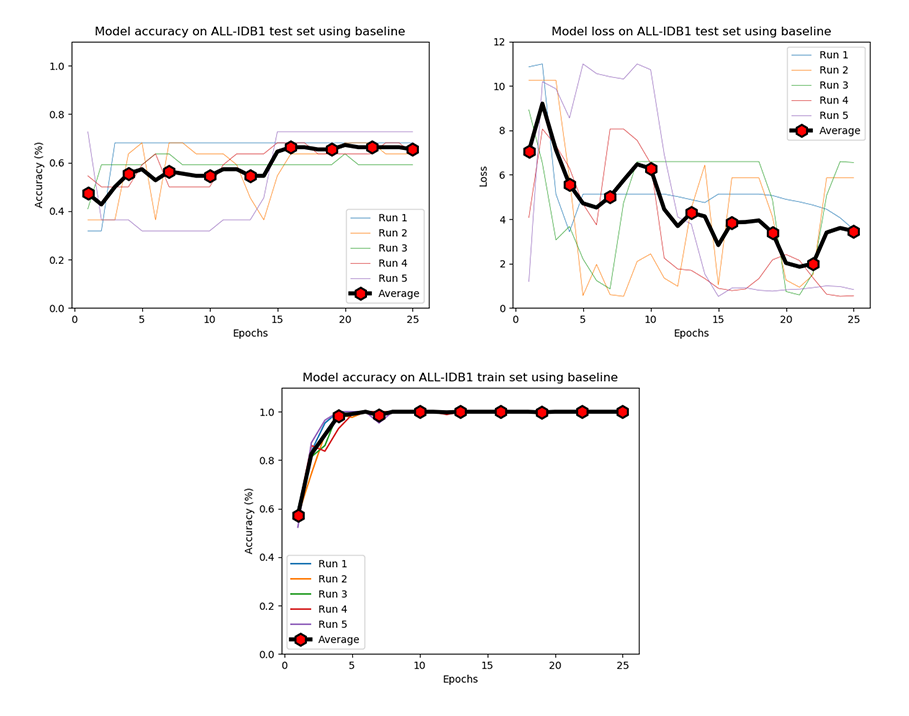
\includegraphics[scale=0.5]{Code/ch6-LeukemiaSubtypes/figures_result/ALL_IDB1/all_idb1-baseline.PNG}
  \caption{Results of experiment A.1 (On ALL-IDB1, with Baseline) - The average result of the 5 runs after 25 epochs: (1) Accuracy on test set: \textbf{65.45\%} (2) Loss value on test set: \textbf{3.46} (3) Accuracy on train set: \textbf{100\%}}
  \label{fig:results-A1}
\end{figure}


\subsubsection{Experiment A.2 - Filters}
In this experiment, we keep the baseline CNN but we preprocess the images of the resized dataset by applying some filters \textbf{separately}. \\

\textbf{Greyscale}

First filter that we apply is transforming the images into greyscale. The results obtained when using greyscale images is very bad. It stucks to 50\% which means a totally random prediction. This issue can be due the fact that images are already very small and we suppress the color feature that seems to be important in such images. In fact, the original images (with color) of ALL-IDB1 dataset are at first sight very similar. One of the main feature that distinct them is color. Adding such greyscale filter transforms the images into "mirror" images that causes a total fuzziness whether for human eyes or the CNN model. \\ 

\textbf{Contrast increased} 

The second filter we apply is to increase the contrast of the images by an arbitrary value. In our case, we will increase the contrast by 4. As illustrated in \autoref{fig:preproc-leuk}(b), the color and the edges of blood cells are more highlighted. These features constitute important information for such classification. Bringing them to light can therefore only be a good idea. This affirmation is well confirmed by the results obtained. In average, we obtain an accuracy of 84.54\% after 25 epochs which is even more than the baseline result of the reference article presented in the previous section. Hence, the size of the images seems to not be the most important feature in such images as we obtain in average better results by increasing the images' contrast to highlight the blood cells color and edges on 100x100 images. However, we will take a look on the size feature on \autoref{sec:size-allidb1}. \\

\textbf{Histogram equalization} 

Finally, the last filter that we apply is a well-known image enhancement technique called \textit{histogram equalization} and previously explained in \autoref{sec:img-enhancement-breast}. In summary, what histogram equalization do is increasing the contrast of an image by effectively spreading out the most frequent intensity values of the histogram. This technique is known to be efficient in image recognition problems. This allows for areas of lower local contrast to gain a higher contrast. The results obtained (average of 90.9\%) do not betray the reputation for image enhancement of the histogram equalization technique. In contrary to the previous filter where we apply the same contrast increase on the entire image, here we only increase the contrast where it is needed. Therefore, we obtain clearer images that may highlight efficiently affected blood cells and help for the model's learning.  

\vspace{1cm}

\begin{center}
\begin{tabular}{|l|c|c|c|}
  \hline
   & \textbf{Greyscale} & \textbf{Increased contrast} & \textbf{Histogram equalization} \\
  \hline
  Accuracy on test set & 51.81\% & 84.54\% & 90.9\% \\
  Loss value on test set & 6.09 & 1.43 &  0.28\\ 
  Accuracy on train set & 100\% & 100\% & 100\% \\ 
  \hline
\end{tabular}
\captionof{table}{Experiment A.2 (On ALL-IDB1, with filters applied) - Train set = 86 images, Test set = 22 images - Average results for each filters applied separately after 25 epochs. ACC-TEST is the accuracy result on test set, LOSS-TEST the value of cost function on test set and ACC-TRAIN the accuracy result on train set.}
\label{table:results-A2}
\end{center}

\begin{figure}[H]
  \centering
  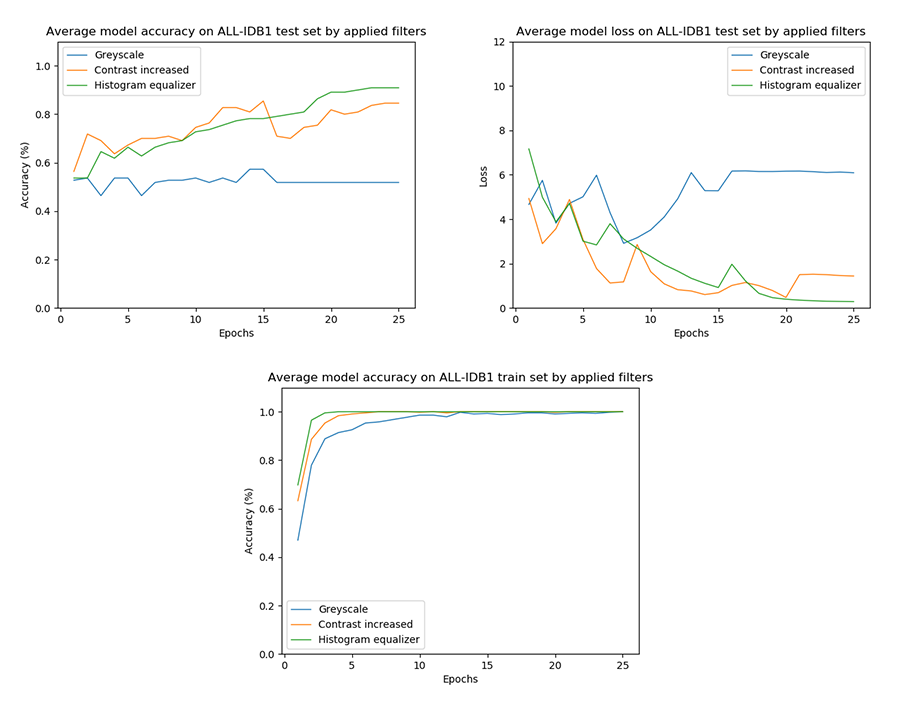
\includegraphics[scale=0.5]{Code/ch6-LeukemiaSubtypes/figures_result/ALL_IDB1/all_idb1-filters.PNG}
  \caption{Results of experiment A.2 (On ALL-IDB1, with filters applied). The results presented are the average of 5 different runs for each filter applied.}
  \label{fig:results-A2}
\end{figure}

\subsubsection{Experiment A.3 - Size 200x200} \label{sec:size-allidb1}
The results that we have obtained using the baseline CNN and a resize of the images by 100x100 were not as good as the reference article \cite{leukemia} even though they were still correct. An hypothesis of this issue would have been the size of these images. This experiment aims to test the size feature for the learning of the model. To do that, we have then use the same baseline CNN as before but here with a preprocessing of 200x200. The images contains now 40000 pixels which is 4 times more than in experiment A.1.

Nevertheless, what we can observe from the results is that it does not enhance the accuracy on test set and has lower results in average. These results thus does not allow to draw a positive conclusion about the effectiveness of using larger images. Looking to the graphs, we can observe that the accuracy has a continuous behaviour and the model seems not to learn more along epochs. This can be due to the number of images of our training set (86 images) which does not allow the model to learn efficiently larger images. 

\newpage
\begin{center}
\begin{tabular}{|l|c|c|c|c|c|c|}
  \hline
   & \textbf{Run 1} & \textbf{Run 2} & \textbf{Run 3} & \textbf{Run 4} & \textbf{Run 5} & \textbf{AVG}\\
  \hline
  ACC-TEST & 63.63\% & 40.9\% & 54.54\% & 77.27\% & 59.09\% & 59.08\%\\
  LOSS-TEST & 2.47 & 5.94 & 1.96 & 0.51  & 0.96 & 2.36 \\ 
  ACC-TRAIN & 100\% & 100\% & 100\% & 100\% & 100\% & 100\% \\ 
  \hline
\end{tabular}
\captionof{table}{Experiment A.3 (On ALL-IDB1, with larger resize) - Train set = 86 images, Test set = 22 images - Detailed results of each run after 25 epochs. ACC-TEST is the accuracy result on test set, LOSS-TEST the value of cost function on test set and ACC-TRAIN the accuracy result on train set.}
\label{table:results-A3}
\end{center}

\begin{figure}[H]
  \centering
  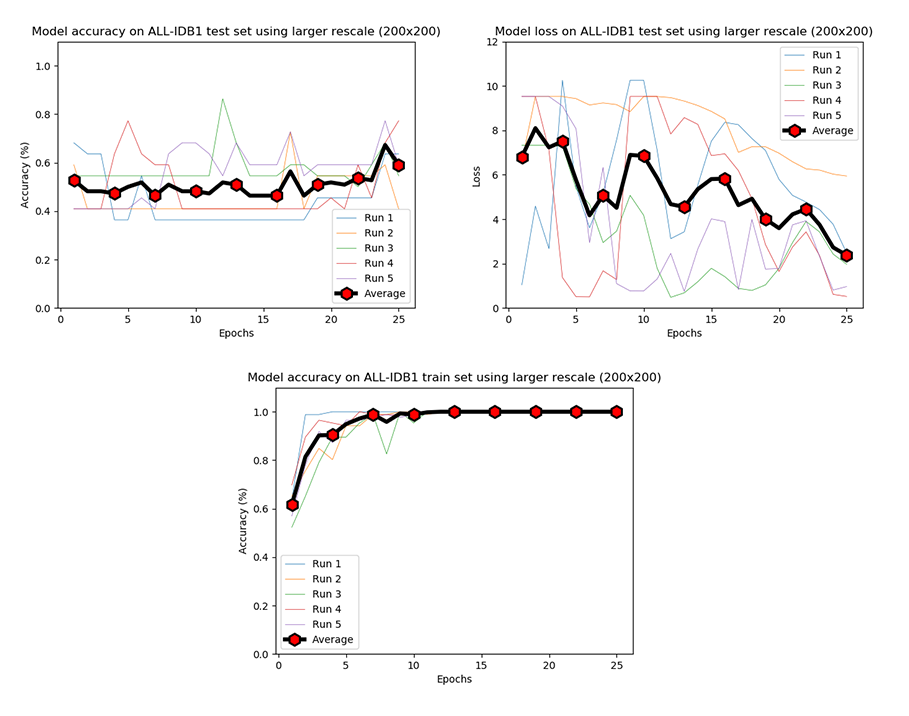
\includegraphics[scale=0.5]{Code/ch6-LeukemiaSubtypes/figures_result/ALL_IDB1/all_idb1-200x200.PNG}
  \caption{Results of experiment A.3 (On ALL-IDB1, with larger resize 200x200) - The average result of the 5 runs after 25 epochs: (1) Accuracy on test set: \textbf{68.45\%} (2) Loss value on test set: \textbf{0.992} (3) Accuracy on train set: \textbf{100\%}}
  \label{fig:results-A3}
\end{figure}


\subsubsection{Experiment A.4 - Noise} \label{sec:noise-allidb1}

A recurrent question was about how the model reacts to noise. In this experiment, we try different level of gaussian noise added. Respectively, we try the following values of noise: [0.1,0.2,0.4,0.6,0.8]. In \autoref{sec:noise-cifar}, we have seen that noise can be used as regularization if used sparingly. Is that also valid for medical images? 

Following the results, we can mention that this regularization effect is still valid if a very small value of noise is applied, not more than 0.2. From 0.4, we begin to see bad impact of noise such that the model is not even capable to reach 100\% accuracy on training set after 25 epochs. Moreover, on the third graph representing the learning speed of the model (accuracy on train set) we can observe the more noise applied, the slower the model is to converge. Thus, the threshold noise value to have a regularization effect should be 0.2. Above this, the value of cost function is increasing constantly which means that the model is making lot of error between predicted values and expected values. The model has wrong abilities to estimate the relationship between the label and the input. 

This is also verified when looking to the accuracy results on test set. From \texttt{noise=0.4}, we approach to a prediction rate of 50\% the total prediction randomness.    

\begin{center}
\begin{tabular}{|l|c|c|c|c|c|c|}
  \hline
   & \textbf{noise=0.1} & \textbf{noise=0.2} & \textbf{noise=0.4} & \textbf{noise=0.6} & \textbf{noise=0.8}\\
  \hline
  ACC-TEST & 77.27\% & 63.63\% & 59.09\% & 59.09\% & 54.54\%\\
  LOSS-TEST & 0.67 & 1.64 & 1.75 & 4.33  & 7.32\\ 
  ACC-TRAIN & 100\% & 100\% & 97.67\% & 94.18\% & 84.88\% \\ 
  \hline
\end{tabular}
\captionof{table}{Experiment A.4 (On ALL-IDB1, with different level of noise) - Train set = 86 images, Test set = 22 images - Average results depending on noise level. ACC-TEST is the accuracy result on test set, LOSS-TEST the value of cost function on test set and ACC-TRAIN the accuracy result on train set.}
\label{table:results-A4}
\end{center}

\begin{figure}[H]
  \centering
  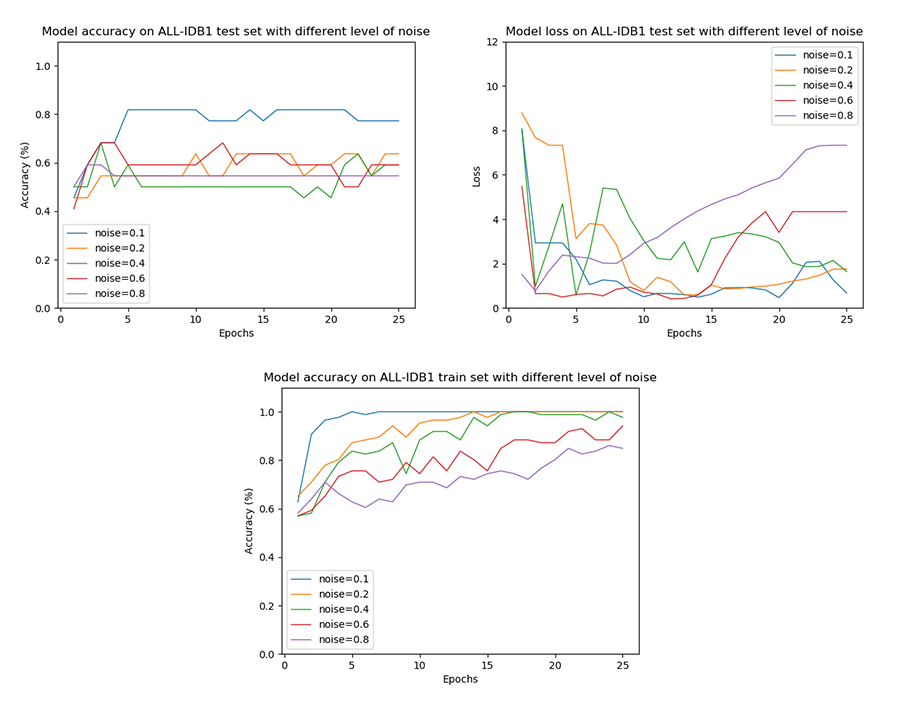
\includegraphics[scale=0.45]{Code/ch6-LeukemiaSubtypes/figures_result/ALL_IDB1/all_idb1-noise.PNG}
  \caption{Results of experiment A.4 (On ALL-IDB1, with different level of noise). The results presented are the average of 5 different runs for each noise level.}
  \label{fig:results-A4}
\end{figure}


\subsubsection{Experiment A.5 - Dropout}
As reminder, dropout is a regularization technique that consists to drop some neurons during the training phase (see \autoref{sec:dropout-cifar} for more information). It is generally used to counter overfitting. When we have used it on CIFAR-10 dataset constituted of 50000 images for training, it had very good impact on the learning phase. Here, we have only 86 images for training which is very low, will it be as efficient as using it on large dataset such as CIFAR-10? Obviously no. On such a small dataset, the model does not suffer from overfitting but more about underfitting. Using dropout is then a very bad idea since it takes out neurons to the model and make it way more difficult to learn. The results obtained show it well. We have high losses values and bad accuracy rates. Looking to this last on test set graph, we observe a continuous behaviour around 50\% rate. Same for the accuracy on train set, it reaches in average 61.85\% accuracy after 25 epochs. That shows the disability for the model to learn correctly.  


\begin{center}
\begin{tabular}{|l|c|c|c|c|c|c|}
  \hline
   & \textbf{Run 1} & \textbf{Run 2} & \textbf{Run 3} & \textbf{Run 4} & \textbf{Run 5} & \textbf{AVG}\\
  \hline
  ACC-TEST & 59.09\% & 40.9\% & 50.00\% & 59.09\% & 63.63\% & 54.54\% \\
  LOSS-TEST & 1.07 & 9.52 & 8.05 & 6.11  & 4.15 & 5.78 \\ 
  ACC-TRAIN & 62.79\% & 58.13\% & 54.65\% & 60.46\% & 73.25\% & 61.85\% \\ 
  \hline
\end{tabular}
\captionof{table}{Experiment A.5 (On ALL-IDB1, with dropout=0.1) - Train set = 86 images, Test set = 22 images - Detailed results of each run after 25 epochs. ACC-TEST is the accuracy result on test set, LOSS-TEST the value of cost function on test set and ACC-TRAIN the accuracy result on train set.}
\label{table:results-A5}
\end{center}


\begin{figure}[H]
  \centering
  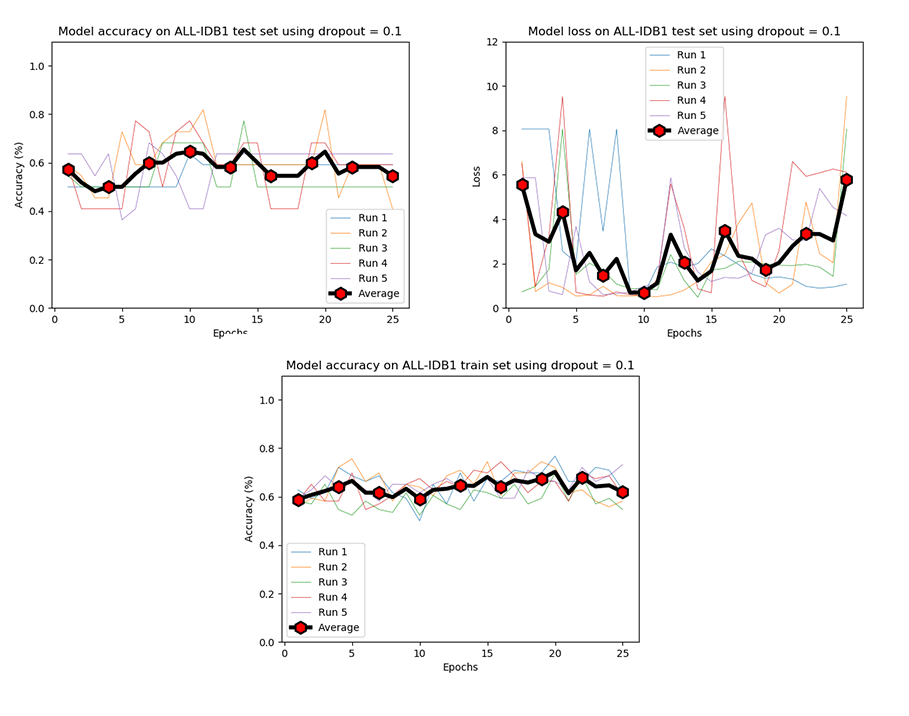
\includegraphics[scale=0.4]{Code/ch6-LeukemiaSubtypes/figures_result/ALL_IDB1/all_idb1-dropout.PNG}
  \caption{Results of experiment A.5 (On ALL-IDB1, with dropout=0.1) - The average result of the 5 runs after 25 epochs: (1) Accuracy on test set: \textbf{54.54\%} (2) Loss value on test set: \textbf{5.78} (3) Accuracy on train set: \textbf{61.85\%}}
  \label{fig:results-A5}
\end{figure}


\subsubsection{Experiment A.6 - Data augmentation}

In this experiment, we have used data augmentation in order to expand the dataset. The method used is explained in \autoref{sec:data-aug-leuk}. The results obtained are quite good and show well the efficiency of using data augmentation. In average, we gain 7\% accuracy and have low loss value when using data augmentation. The images' direction and sense seems to not disturb the model's learning and looks like it is not an impacting feature to determinate the label. 

Nevertheless, some runs as run 4 show an unconvincing performance (63.63\%). This can be due to a type of image augmentation used: rotations. In fact, rotations create some black area and represents a considerable percentage of the image. Thus, the model could have taken it in account and considers it as a feature of the corresponding label which confuses the learning of the model. As data augmentation is done randomly between all the types of image augmentation explained previously, this run could have been implied by this issue and then impact negatively the learning and prediction.     

\begin{center}
\begin{tabular}{|l|c|c|c|c|c|c|}
  \hline
   & \textbf{Run 1} & \textbf{Run 2} & \textbf{Run 3} & \textbf{Run 4} & \textbf{Run 5} & \textbf{AVG}\\
  \hline
  ACC-TEST & 72.72\% & 81.81\% & 65.9\% & 63.63\% & 77.27\% & 72.26\% \\
  LOSS-TEST & 1.17 & 0.46 & 1.25 & 2.76  & 0.91 & 1.31 \\ 
  ACC-TRAIN & 98.83\% & 100\% & 100\% & 99.41\% & 100\% & 99.64\% \\ 
  \hline
\end{tabular}
\captionof{table}{Experiment A.6 (On ALL-IDB1, with data augmentation) - Train set = 172 images, Test set = 44 images - Detailed results of each run after 25 epochs. ACC-TEST is the accuracy result on test set, LOSS-TEST the value of cost function on test set and ACC-TRAIN the accuracy result on train set.}
\label{table:results-A6}
\end{center}


\begin{figure}[H]
  \centering
  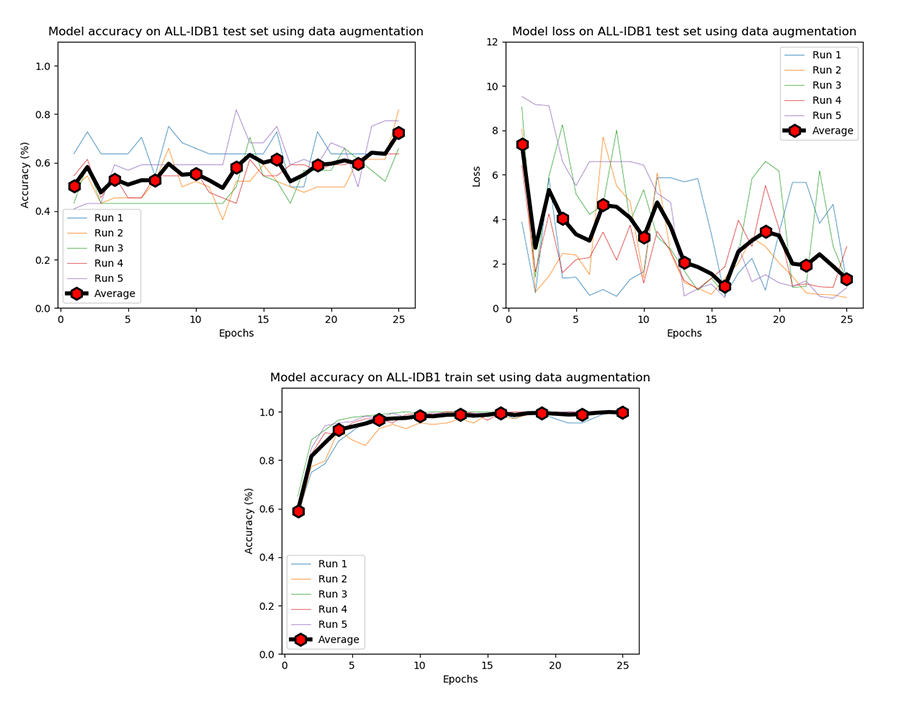
\includegraphics[scale=0.38]{Code/ch6-LeukemiaSubtypes/figures_result/ALL_IDB1/all_idb1-data_aug.PNG}
  \caption{Results of experiment A.6 (On ALL-IDB1, with data augmentation) - The average result of the 5 runs after 25 epochs: (1) Accuracy on test set: \textbf{72.26\%} (2) Loss value on test set: \textbf{1.31} (3) Accuracy on train set: \textbf{99.64\%}}
  \label{fig:results-A6}
\end{figure}


\subsubsection{Experiment A.7 - Dropout and data augmentation} \label{sec:drop-dataaug-allidb1}
A problem of using dropout was the size of our training set. If we use larger dataset using data augmentation, will dropout be more efficient this time? In this experiment, we try to combine dropout and data augmentation. However, from what we can observe by the results, dropout is still counterproductive for the model's learning. Even if the results are more encouraging than experiment A.5 where we use only dropout, they are still not as good as using only data augmentation. That shows that the model is still not overfit and need way more data to suffer from it in order to have regularization effect while using dropout. 


\begin{center}
\begin{tabular}{|l|c|c|c|c|c|c|}
  \hline
   & \textbf{Run 1} & \textbf{Run 2} & \textbf{Run 3} & \textbf{Run 4} & \textbf{Run 5} & \textbf{AVG}\\
  \hline
  ACC-TEST & 54.54\% & 59.09\% & 77.27\% & 65.9\% & 72.72\% & 65.9\% \\
  LOSS-TEST & 1.13 & 1.95 & 0.84 & 1.21 & 0.7 & 1.16 \\ 
  ACC-TRAIN & 64.53\% & 65.11\% & 68.60\% & 58.72\% & 68.02\% & 64.99\% \\ 
  \hline
\end{tabular}
\captionof{table}{Experiment A.7 (On ALL-IDB1, with data augmentation and dropout=0.1) - Train set = 172 images, Test set = 44 images - Detailed results of each run after 25 epochs. ACC-TEST is the accuracy result on test set, LOSS-TEST the value of cost function on test set and ACC-TRAIN the accuracy result on train set.}
\label{table:results-A7}
\end{center}


\begin{figure}[H]
  \centering
  \includegraphics[scale=0.4]{Code/ch6-LeukemiaSubtypes/figures_result/ALL_IDB1/all_idb1-data_aug_dropout.PNG}
  \caption{Results of experiment A.7 (On ALL-IDB1, with data augmentation and dropout=0.1) - The average result of the 5 runs after 25 epochs: (1) Accuracy on test set: \textbf{65.9\%} (2) Loss value on test set: \textbf{1.16} (3) Accuracy on train set: \textbf{64.99\%}}
  \label{fig:results-A7}
\end{figure}


\newpage
\subsubsection{Summary and conclusion for ALL-IDB1 dataset experiments}
% Tableau qui récapitule tous les résultats au dessus + conclusion
To summarize the experiments done using ALL-IDB1 dataset, the \autoref{table:summary-allidb1} recapitulates the average results of each experiment for the accuracy on test and train set as well as the loss value for test set. 

As the dataset is very small using small images, using the simplest CNN is the best way to learn efficiently. To make the significant features clearer, a preprocessing step using image enhancement (contrast increasing or histogram equalization) seems to be very efficient. Hence, the best result obtained uses the baseline CNN on enhanced images by histogram equalization. We obtain an average of 90.9\% accuracy on test set and a loss value of 0.28. 

On the other hand, the worst result is obtained by adding a huge value of noise (0.8). We obtain an average of 54.54\% accuracy on test set and a loss value of 7.32. This average accuracy is also obtained when using dropout without data augmentation. This shows how much using dropout is bad when having such a small dataset (comparable to adding 0.8 of gaussian noise!).  


\begin{center}
\begin{tabular}{|c|c|c|c|}
  \hline
          & \textbf{ACC-TEST} & \textbf{LOSS-TEST} & \textbf{ACC-TRAIN} \\
  \hline
  Exp A.1 & 65.45\% & 3.46 & 100\% \\
  \hline
  Exp A.2 (grey) & 51.81\% & 6.09 & 100\%  \\ 
  Exp A.2 (contrast) & 84.54\% & 1.43 & 100\% \\ 
  Exp A.2 (hist. eq.) & \textcolor{ForestGreen}{90.9\%} & \textcolor{ForestGreen}{0.28} & 100\% \\ 
  \hline
  Exp A.3 & 59.08\% & 2.36 & 100\% \\
  \hline
  Exp A.4 (noise=0.1) & 77.27\% & 0.67 & 100\%  \\ 
  Exp A.4 (noise=0.2) & 63.63\% & 1.64 & 100\% \\ 
  Exp A.4 (noise=0.4) & 59.09\% & 1.75 & 97.67\% \\
  Exp A.4 (noise=0.6) & 59.09\% & 4.33 & 94.18\%  \\ 
  Exp A.4 (noise=0.8) & \textcolor{red}{54.54\%} & \textcolor{red}{7.32} & 84.88\% \\
  \hline 
  Exp A.5 & \textcolor{red}{54.54\%} & 5.78 & 61.85\% \\
  \hline
  Exp A.6 & 72.26\% & 1.31 & 99.64\% \\
  \hline
  Exp A.7 & 65.9\% & 1.16 & 64.99\% \\ 
  \hline
\end{tabular}
\captionof{table}{Summary of the results obtained for ALL-IDB1. The results presented in this table are the average results for each experiment. ACC-TEST is the accuracy result on test set, LOSS-TEST the value of cost function on test set and ACC-TRAIN the accuracy result on train set. The result highlighted in \textcolor{ForestGreen}{green} is the best result obtained. The result highlighted in \textcolor{red}{red} is the worst result obtained.}
\label{table:summary-allidb1}
\end{center}


\subsection{Case B - ALL-IDB2}

Compared to ALL-IDB1, ALL-IDB2 has been already preprocessed by image segmentation on the region of interest (ROI). This dataset contains 260 images that focus on an unique blood cell. We then have 208 images for training and 52 images for testing when not using data augmentation. Otherwise, we have 416 images for training and 104 for testing. Again, more information are described in \autoref{sec:all-idb}. We aim then to compare results without segmentation (ALL-IDB1) and results with segmentation (ALL-IDB2) to observe the efficiency of such preprocessing. To do that, we will do the same experiments as ALL-IDB1. The images of the dataset have also been resized to 100x100, their original sizes were 257x257.

\subsubsection{Experiment B.1 - Baseline}
When using baseline CNN on the original resized dataset, the results seems to be worse than when we use ALL-IDB1 but still around 62-65\% accuracy. At first sight, determinate if the patient is affected by the disease by using only an unique blood cell is more difficult as we use a more global view of multiple blood cells to determinate if the patient is affected by the disease or not. The features that determinates the label may be more accurate when the only information given is a blood cell, i.e blood cells are very similar to each other. Therefore, we need a larger dataset to obtain better results. Nevertheless can we make these features more impacting to the model? That is what we will observe in the next section by using some filters.  

\begin{center}
\begin{tabular}{|l|c|c|c|c|c|c|}
  \hline
   & \textbf{Run 1} & \textbf{Run 2} & \textbf{Run 3} & \textbf{Run 4} & \textbf{Run 5} & \textbf{AVG}\\
  \hline
  ACC-TEST & 63.46\% & 63.46\% & 67.3\% & 55.76\% & 59.61\% & 61.91\% \\
  LOSS-TEST & 3.22 & 0.65 & 0.79 & 2.59  & 2.05 & 1.86 \\ 
  ACC-TRAIN & 100\% & 100\% & 100\% & 100\% & 100\% & 100\% \\ 
  \hline
\end{tabular}
\captionof{table}{Experiment B.1 (On ALL-IDB2, with Baseline) - Train set = 208 images, Test set = 52 images - Detailed results of each run after 25 epochs. ACC-TEST is the accuracy result on test set, LOSS-TEST the value of cost function on test set and ACC-TRAIN the accuracy result on train set.}
\label{table:results-B1}
\end{center}

\begin{figure}[H]
  \centering
  \includegraphics[scale=0.42]{Code/ch6-LeukemiaSubtypes/figures_result/ALL_IDB2/all_idb2-baseline.PNG}
  \caption{Results of experiment B.1 (On ALL-IDB2, with Baseline) - The average result of the 5 runs after 25 epochs: (1) Accuracy on test set: \textbf{61.91\%} (2) Loss value on test set: \textbf{1.86} (3) Accuracy on train set: \textbf{100\%}}
  \label{fig:results-B1}
\end{figure}

\subsubsection{Experiment B.2 - Filters}
Same as ALL-IDB1, we will experiment 3 different filters: transforming images into greyscale, increasing images' contrast with an arbitrary value of 4 and using histogram equalization on the images. \\

\textbf{Greyscale}

In contrary to ALL-IDB1, here we obtain more convincing results. As we manage only one blood cell, transforming the images into greyscale allow the model to highlight the shapes/edges of the cell and its content more clearly. \\ 

\textbf{Contrast increased}

Same as ALL-IDB1, increase the contrast to the images seems to be a good image enhancement technique. Again, edges and shapes are highlighted and facilitates the model's learning. \\ 

\textbf{Histogram equalization}

This time, histogram equalization does not give the best results even though it still gives very good ones. Histogram equalization technique is then a safe method to enhance correctly the image without making it unreadable unlike if we put a too large contrast increase value.

\vspace{1cm}

\begin{center}
\begin{tabular}{|l|c|c|c|}
  \hline
   & \textbf{Greyscale} & \textbf{Increased contrast} & \textbf{Histogram equalization} \\
  \hline
  Accuracy on test set & 71.53\% & 80.38\% & 73.84\% \\
  Loss value on test set & 1.09 & 0.47 &  0.95\\ 
  Accuracy on train set & 99.9\% & 100\% & 100\% \\ 
  \hline
\end{tabular}
\captionof{table}{Experiment B.2 (On ALL-IDB2, with filters applied) - Train set = 208 images, Test set = 52 images - Average results for each filters applied separately after 25 epochs. ACC-TEST is the accuracy result on test set, LOSS-TEST the value of cost function on test set and ACC-TRAIN the accuracy result on train set.}
\label{table:results-B2}
\end{center}

\newpage
\hspace*{0mm}\vfill
\begin{figure}[H]
  \centering
  \includegraphics[scale=0.5]{Code/ch6-LeukemiaSubtypes/figures_result/ALL_IDB2/all_idb2-filters.PNG}
  \caption{Results of experiment B.2 (On ALL-IDB2, with filters applied). The results presented are the average of 5 different runs for each filter applied.}
  \label{fig:results-B2}
\end{figure}
\vfill\hspace*{0mm}

\newpage
\subsubsection{Experiment B.3 - Size 200x200}
The original images from ALL-IDB2 dataset have a size of 257x257. In this section, we will use 200x200 images and can then be considered as the original size. For ALL-IDB1, we have seen that enlarge the images was not the best method to increase the performance due to the very small numbers of samples contained in the dataset. Here for ALL-IDB2, we have 2 times more images and we use the original size of the dataset. So that, we can observe that we obtain slightly better results. Using larger images when having much samples seems then to be a good idea and constitutes a good asset to feature detection.    


\begin{center}
\begin{tabular}{|l|c|c|c|c|c|c|}
  \hline
   & \textbf{Run 1} & \textbf{Run 2} & \textbf{Run 3} & \textbf{Run 4} & \textbf{Run 5} & \textbf{AVG}\\
  \hline
  ACC-TEST & 69.23\% & 65.38\% & 75.00\% & 67.3\% & 57.69\% & 66.92\%\\
  LOSS-TEST & 0.52 & 0.68 & 0.65 & 0.94  & 1.23 & 0.804 \\ 
  ACC-TRAIN & 100\% & 100\% & 100\% & 99.51\% & 100\% & 99.902\% \\ 
  \hline
\end{tabular}
\captionof{table}{Experiment B.3 (On ALL-IDB2, with larger resize) - Train set = 208 images, Test set = 52 images - Detailed results of each run after 25 epochs. ACC-TEST is the accuracy result on test set, LOSS-TEST the value of cost function on test set and ACC-TRAIN the accuracy result on train set.}
\label{table:results-B3}
\end{center}

\begin{figure}[H]
  \centering
  \includegraphics[scale=0.45]{Code/ch6-LeukemiaSubtypes/figures_result/ALL_IDB2/all_idb2-200x200.PNG}
  \caption{Results of experiment B.3 (On ALL-IDB2, with larger resize 200x200) - The average result of the 5 runs after 25 epochs: (1) Accuracy on test set: \textbf{68.92\%} (2) Loss value on test set: \textbf{0.804} (3) Accuracy on train set: \textbf{99.902\%}}
  \label{fig:results-B3}
\end{figure}



\subsubsection{Experiment B.4 - Noise}
Overall, the results seems to have the same behaviour than the results when using ALL-IDB1 dataset. At first, we have a regularization effect when using small noise value. But when using a too large value -- here still 0.4, noise has a very bad impact on the model's learning. At this time, loss values are exploding and almost grow exponentially. The explanations from \autoref{sec:noise-allidb1} are also valid for ALL-IDB2.

\begin{center}
\begin{tabular}{|l|c|c|c|c|c|c|}
  \hline
   & \textbf{noise=0.1} & \textbf{noise=0.2} & \textbf{noise=0.4} & \textbf{noise=0.6} & \textbf{noise=0.8}\\
  \hline
  ACC-TEST & 71.15\% & 63.46\% & 50.00\% & 55.76\% & 46.13\%\\
  LOSS-TEST & 1.41 & 2.34 & 3.60 & 6.45  & 7.12\\ 
  ACC-TRAIN & 100\% & 99.5\% & 98.55\% & 97.55\% & 94.71\% \\ 
  \hline
\end{tabular}
\captionof{table}{Experiment B.4 (On ALL-IDB2, with different level of noise) - Train set = 208 images, Test set = 52 images - Average results depending on noise level. ACC-TEST is the accuracy result on test set, LOSS-TEST the value of cost function on test set and ACC-TRAIN the accuracy result on train set.}
\label{table:results-B4}
\end{center}

\begin{figure}[H]
  \centering
  \includegraphics[scale=0.5]{Code/ch6-LeukemiaSubtypes/figures_result/ALL_IDB2/all_idb2-noise.PNG}
  \caption{Results of experiment B.4 (On ALL-IDB2, with different level of noise). The results presented are the average of 5 different runs for each noise level.}
  \label{fig:results-B4}
\end{figure}


\subsubsection{Experiment B.5 - Dropout}
Using dropout when your dataset is very small is a technique to forget: that is the conclusion that we have made after the experiment A.5 using dropout on ALL-IDB1 that contains only 108 images. Here we have a little bit much images on ALL-IDB2 and we can remark that overall it still has bad results but we can see a little augmentation on average training set accuracy results. That reinforces the idea that dropout begins to have a regularization effect when we have very large datasets. That is an additional proof of this assertion that we have done previously in experiment A.7 (see \autoref{sec:drop-dataaug-allidb1}). Of course, for this case, we are far from having a dataset size conductive to dropout as regularizer. That explains the bad results.  

\begin{center}
\begin{tabular}{|l|c|c|c|c|c|c|}
  \hline
   & \textbf{Run 1} & \textbf{Run 2} & \textbf{Run 3} & \textbf{Run 4} & \textbf{Run 5} & \textbf{AVG}\\
  \hline
  ACC-TEST & 55.76\% & 53.84\% & 48.07\% & 51.92\% & 67.30\% & 55.37\% \\
  LOSS-TEST & 1.25 & 1.58 & 2.40 & 3.57  & 0.7 & 1.9 \\ 
  ACC-TRAIN & 73.07\% & 70.67\% & 64.42\% & 62.5\% & 70.0\% & 68.12\% \\ 
  \hline
\end{tabular}
\captionof{table}{Experiment B.5 (On ALL-IDB2, with dropout=0.1) - Train set = 208 images, Test set = 52 images - Detailed results of each run after 25 epochs. ACC-TEST is the accuracy result on test set, LOSS-TEST the value of cost function on test set and ACC-TRAIN the accuracy result on train set.}
\label{table:results-B5}
\end{center}


\begin{figure}[H]
  \centering
  \includegraphics[scale=0.45]{Code/ch6-LeukemiaSubtypes/figures_result/ALL_IDB2/all_idb2-dropout.PNG}
  \caption{Results of experiment B.5 (On ALL-IDB2, with dropout=0.1) - The average result of the 5 runs after 25 epochs: (1) Accuracy on test set: \textbf{55.37\%} (2) Loss value on test set: \textbf{1.9} (3) Accuracy on train set: \textbf{68.12\%}}
  \label{fig:results-B5}
\end{figure}



\subsubsection{Experiment B.6 - Data augmentation}

One more time, data augmentation shows having a good impact on model's performance. These experiments give some indications about the efficiency of data augmentation especially when using small datasets like ALL-IDB1 or ALL-IDB2. This data augmentation techniques give many more samples to the dataset and allow the model to learn more in order to make better predictions. 

Furthermore, the different image manipulations that we have done during this data augmentation seems to not be impacting negatively the feature detection step whether for segmented and non-segmented images. Thus, data augmentation constitutes a must-use asset to increase the performance of the model.  

\begin{center}
\begin{tabular}{|l|c|c|c|c|c|c|}
  \hline
   & \textbf{Run 1} & \textbf{Run 2} & \textbf{Run 3} & \textbf{Run 4} & \textbf{Run 5} & \textbf{AVG}\\
  \hline
  ACC-TEST & 64.42\% & 75.96\% & 72.11\% & 67.30\% & 79.80\% & 71.91\% \\
  LOSS-TEST & 1.44 & 0.67 & 1.30 & 1.67 & 0.91 & 1.198 \\ 
  ACC-TRAIN & 99.75\% & 99.75\% & 100\% & 100\% & 100\% & 99.9\% \\ 
  \hline
\end{tabular}
\captionof{table}{Experiment B.6 (On ALL-IDB2, with data augmentation) - Train set = 416 images, Test set = 104 images - Detailed results of each run after 25 epochs. ACC-TEST is the accuracy result on test set, LOSS-TEST the value of cost function on test set and ACC-TRAIN the accuracy result on train set.}
\label{table:results-B6}
\end{center}

\begin{figure}[H]
  \centering
  \includegraphics[scale=0.45]{Code/ch6-LeukemiaSubtypes/figures_result/ALL_IDB2/all_idb2-data_aug.PNG}
  \caption{Results of experiment B.6 (On ALL-IDB2, with data augmentation) - The average result of the 5 runs after 25 epochs: (1) Accuracy on test set: \textbf{71.91\%} (2) Loss value on test set: \textbf{1.198} (3) Accuracy on train set: \textbf{99.9\%}}
  \label{fig:results-B6}
\end{figure}


\subsubsection{Experiment B.7 - Dropout and data augmentation}

Similarly to the experiments on dropout, we observe the same issue as usual when using dropout on small datasets. The model cannot learn correctly to the neurons removed and cannot reach more than 70\% accuracy on training set. As this issue was explained before, refer to experiments A.5, A.7 and B.5 for more explanations. 

\begin{center}
\begin{tabular}{|l|c|c|c|c|c|c|}
  \hline
   & \textbf{Run 1} & \textbf{Run 2} & \textbf{Run 3} & \textbf{Run 4} & \textbf{Run 5} & \textbf{AVG}\\
  \hline
  ACC-TEST & 66.34\% & 64.42\% & 58.65\% & 65.38\% & 68.26\% & 64.61\% \\
  LOSS-TEST & 0.79 & 0.7 & 0.93 & 1.53 & 0.926 & 0.97 \\ 
  ACC-TRAIN & 67.22\% & 66.74\% & 64.33\% & 62.16\% & 65.78\% & 65.24\% \\ 
  \hline
\end{tabular}
\captionof{table}{Experiment B.7 (On ALL-IDB2, with data augmentation and dropout=0.1) - Train set = 416 images, Test set = 104 images - Detailed results of each run after 25 epochs. ACC-TEST is the accuracy result on test set, LOSS-TEST the value of cost function on test set and ACC-TRAIN the accuracy result on train set.}
\label{table:results-B7}
\end{center}


\begin{figure}[H]
  \centering
  \includegraphics[scale=0.5]{Code/ch6-LeukemiaSubtypes/figures_result/ALL_IDB2/all_idb2-data_aug_dropout.PNG}
  \caption{Results of experiment B.7 (On ALL-IDB2, with data augmentation and dropout=0.1) - The average result of the 5 runs after 25 epochs: (1) Accuracy on test set: \textbf{65.9\%} (2) Loss value on test set: \textbf{1.16} (3) Accuracy on train set: \textbf{64.99\%}}
  \label{fig:results-B7}
\end{figure}

\subsubsection{Summary and conclusion for ALL-IDB2 dataset experiments}
To conclude the different experiments done using ALL-IDB2 dataset, the preprocessing step using image segmentation do not show a clear advantage in comparison with the experiments done using ALL-IDB1 with no segmentation. Overall, the results are quite equivalent. Using contrast augmentation (whether with arbitrary value or with histogram equalization) is the best image enhancement technique to have great performance. On the other hand, adding a huge value of noise still gets the worst results. However, some clear differences can be observed on some experiments such as the experiment A.2 or A.3 which demonstrate way more good performances by using segmentation.  

The \autoref{table:summary-allidb2} summarizes all the average results obtained during the experiments done with ALL-IDB2. 

\begin{center}
\begin{tabular}{|c|c|c|c|}
  \hline
          & \textbf{ACC-TEST} & \textbf{LOSS-TEST} & \textbf{ACC-TRAIN} \\
  \hline
  Exp B.1 & 61.91\% & 1.86 & 100\% \\
  \hline
  Exp B.2 (grey) & 71.53\% & 1.09 & 99.9\%  \\ 
  Exp B.2 (contrast) & \textcolor{ForestGreen}{80.38\%} & \textcolor{ForestGreen}{0.47} & 100\% \\ 
  Exp B.2 (hist. eq.) & 73.84\% & 0.95 & 100\% \\ 
  \hline
  Exp B.3 & 66.92\% & 0.804 & 99.902\% \\
  \hline
  Exp B.4 (noise=0.1) & 71.15\% & 1.41 & 100\%  \\ 
  Exp B.4 (noise=0.2) & 63.46\% & 2.34 & 99.5\% \\ 
  Exp B.4 (noise=0.4) & 50.00\% & 3.60 & 98.55\% \\
  Exp B.4 (noise=0.6) & 59.09\% & 4.33 & 97.55\%  \\ 
  Exp B.4 (noise=0.8) & \textcolor{red}{46.13\%} & \textcolor{red}{7.12} & 94.71\% \\
  \hline 
  Exp B.5 & 55.37\% & 1.9 & 68.12\% \\
  \hline
  Exp B.6 & 71.91\% & 1.198 & 99.9\% \\
  \hline
  Exp B.7 & 64.61\% & 0.97 & 65.24\% \\ 
  \hline
\end{tabular}
\captionof{table}{Summary of the results obtained for ALL-IDB2. The results presented in this table are the average results for each experiment. ACC-TEST is the accuracy result on test set, LOSS-TEST the value of cost function on test set and ACC-TRAIN the accuracy result on train set. The result highlighted in \textcolor{ForestGreen}{green} is the best result obtained. The result highlighted in \textcolor{red}{red} is the worst result obtained.}
\label{table:summary-allidb2}
\end{center}


\subsection{Case C - ALL-IDB and DEMIR-LEUKEMIA datasets}

The last case deals with ALL-IDB and DEMIR-LEUKEMIA datasets which involves 5 classes: HEALTHY (0), ALL (1), AML (2), CLL (3), CML (4). When not using data augmentation, we consider 732 images for training set and 183 for test set. Otherwise, we have 1464 images for training set and 366 for test set. That makes way more samples than two previous cases but here we also have 3 more classes to predict. The prediction accuracy rate that defines the randomness of the model is then 20\% (not 50\% like a binary classification). In the reference article \cite{leukemia}, they have obtained in average an accuracy of 81.74\% for test set, 1.14 of loss value and 99.34\% for train set after 25 epochs using data augmentation and dropout, with SGD optimizer and no preprocessing step (no resize, no filter).    

\subsubsection{Experiment C.1 - Baseline}
Compared to the reference article \cite{leukemia} results mentioned above, we are far from the results obtained. As matter of fact, we only obtain 49.61\% accuracy on test set. Nevertheless, we have to keep in mind that the reference result is obtained with no resizing. When processing a large amount of images and labelled with 5 classes, size matter a lot and allow the model to learn more. Moreover, the images provided in DEMIR-LEUKEMIA dataset contains a lot of variety of images such that some of them contain features that may confuse the learning of the model such as watermarks or bad resolution. Thus, the results obtained with our images resized at 100x100 is not that bad as it is very far from a totally random prediction. It means that the model learns well even if we use very small images. To enhance those results, are more preprocessing steps necessary or do we have to use more images? That is the subject of the next sections.      

\begin{center}
\begin{tabular}{|l|c|c|c|c|c|c|}
  \hline
   & \textbf{Run 1} & \textbf{Run 2} & \textbf{Run 3} & \textbf{Run 4} & \textbf{Run 5} & \textbf{AVG}\\
  \hline
  ACC-TEST & 56.83\% & 39.89\% & 44.8\% & 51.36\% & 55.19\% & 49.61\% \\
  LOSS-TEST & 2.38 & 6.59 & 2.32 & 2.14  & 1.26 & 2.93 \\ 
  ACC-TRAIN & 99.59\% & 99.72\% & 99.72\% & 99.86\% & 99.59\% & 99.69\% \\ 
  \hline
\end{tabular}
\captionof{table}{Experiment C.1 (On ALL-IDB+DEMIR, with Baseline) - Train set = 732 images, Test set = 183 images - Detailed results of each run after 25 epochs. ACC-TEST is the accuracy result on test set, LOSS-TEST the value of cost function on test set and ACC-TRAIN the accuracy result on train set.}
\label{table:results-C1}
\end{center}

\begin{figure}[H]
  \centering
  \includegraphics[scale=0.42]{Code/ch6-LeukemiaSubtypes/figures_result/LEUK-SUBTYPES/leukSub-baseline.PNG}
  \caption{Results of experiment C.1 (On ALL-IDB+DEMIR, with Baseline) - The average result of the 5 runs after 25 epochs: (1) Accuracy on test set: \textbf{49.61\%} (2) Loss value on test set: \textbf{2.93} (3) Accuracy on train set: \textbf{99.69\%}}
  \label{fig:results-C1}
\end{figure}


\subsubsection{Experiment C.2 - Filters}

As we have seen for experiments done for ALL-IDB dataset, image enhancement using filters like greyscale or contrast enhancement seemed like an efficient technique to increase the performance of our model. This observation is confirmed while looking to the results obtained. We really have convincing results and the image enhancement step looks like being mandatory to gain accuracy rate. In this case, the three filters tested achieve quite similar results even if histogram equalization still have slightly better results.  

\begin{center}
\begin{tabular}{|l|c|c|c|}
  \hline
   & \textbf{Greyscale} & \textbf{Increased contrast} & \textbf{Histogram equalization} \\
  \hline
  Accuracy on test set & 59.01\% & 58.68\% & 61.74\% \\
  Loss value on test set & 2.29 & 2.05 &  1.63\\ 
  Accuracy on train set & 99.86\% & 99.72\% & 99.72\% \\ 
  \hline
\end{tabular}
\captionof{table}{Experiment C.2 (On ALL-IDB+DEMIR, with filters applied) - Train set = 732 images, Test set = 183 images - Average results for each filters applied separately after 25 epochs. ACC-TEST is the accuracy result on test set, LOSS-TEST the value of cost function on test set and ACC-TRAIN the accuracy result on train set.}
\label{table:results-C2}
\end{center}


\begin{figure}[H]
  \centering
  \includegraphics[scale=0.5]{Code/ch6-LeukemiaSubtypes/figures_result/LEUK-SUBTYPES/leukSub-filters.PNG}
  \caption{Results of experiment C.2 (On ALL-IDB+DEMIR, with filters applied). The results presented are the average of 5 different runs for each filter applied.}
  \label{fig:results-C2}
\end{figure}


\subsubsection{Experiment C.3 - Size 200x200}

To have an idea about the importance of using larger images in a case where we have more than 2 classes and more images, we do an experiment with the images of the dataset resized to 200x200. We observe a better performance in average and also a very low loss value. That shows the efficiency of using larger images and explain the very good results obtained by the authors of the reference article \cite{leukemia}. Moreover, we can observe that the model arrives to a convergence state as fast as using 100x100 images which means that it is not really constraining for the model's learning. However, the huge drawback of using larger images is the execution time that grow exponentially depending to the images' sizes.  

\begin{center}
\begin{tabular}{|l|c|c|c|c|c|c|}
  \hline
   & \textbf{Run 1} & \textbf{Run 2} & \textbf{Run 3} & \textbf{Run 4} & \textbf{Run 5} & \textbf{AVG}\\
  \hline
  ACC-TEST & 65.02\% & 67.75\% & 56.28\% & 54.09\% & 56.83\% & 59.99\%\\
  LOSS-TEST & 0.97 & 1.36 & 1.65 & 1.45  & 1.04 & 1.29 \\ 
  ACC-TRAIN & 99.72\% & 99.86\% & 99.31\% & 99.72\% & 99.86\% & 99.69\% \\ 
  \hline
\end{tabular}
\captionof{table}{Experiment C.3 (On ALL-IDB+DEMIR, with larger resize) - Train set = 732 images, Test set = 183 images - Detailed results of each run after 25 epochs. ACC-TEST is the accuracy result on test set, LOSS-TEST the value of cost function on test set and ACC-TRAIN the accuracy result on train set.}
\label{table:results-C3}
\end{center}

\begin{figure}[H]
  \centering
  \includegraphics[scale=0.45]{Code/ch6-LeukemiaSubtypes/figures_result/ALL_IDB2/all_idb2-200x200.PNG}
  \caption{Results of experiment C.3 (On ALL-IDB+DEMIR, with larger resize 200x200) - The average result of the 5 runs after 25 epochs: (1) Accuracy on test set: \textbf{59.99\%} (2) Loss value on test set: \textbf{1.29} (3) Accuracy on train set: \textbf{99.69\%}}
  \label{fig:results-C3}
\end{figure}

\subsubsection{Experiment C.4 - Noise}

When testing the ability of the model to learn when noise is added, the previous experiments on ALL-IDB dataset have shown that the performance decreases drastically when adding more than 20\% of noise. In this case, we see that this performance is badly affected already at 20\% of noise added. Indeed, as we have way more classes and then way more features to learn, the model's ability to learn is more impacted. That is well illustrated in the third graph showing the evolution of accuracy rate on training set where we can observe that more noise added, more the model takes time to  reach convergence. Of course, that proportionality impact the accuracy on test set and the cost of loss function that increases depending of noise added which means that the model is getting harder and harder to make the link between the input image and its label.  

\begin{center}
\begin{tabular}{|l|c|c|c|c|c|c|}
  \hline
   & \textbf{noise=0.1} & \textbf{noise=0.2} & \textbf{noise=0.4} & \textbf{noise=0.6} & \textbf{noise=0.8}\\
  \hline
  ACC-TEST & 51.36\% & 32.78\% & 28.41\% & 25.68\% & 14.75\%\\
  LOSS-TEST & 2.83 & 4.23 & 4.92 &  5.64 & 8.80 \\ 
  ACC-TRAIN & 99.59\% & 98.22\% & 97.81\% & 96.17\% & 94.67\% \\ 
  \hline
\end{tabular}
\captionof{table}{Experiment C.4 (On ALL-IDB+DEMIR, with different level of noise) - Train set = 732 images, Test set = 183 images - Average results depending on noise level. ACC-TEST is the accuracy result on test set, LOSS-TEST the value of cost function on test set and ACC-TRAIN the accuracy result on train set.}
\label{table:results-C4}
\end{center}

\begin{figure}[H]
  \centering
  \includegraphics[scale=0.45]{Code/ch6-LeukemiaSubtypes/figures_result/LEUK-SUBTYPES/leukSub-noise.PNG}
  \caption{Results of experiment C.4 (On ALL-IDB+DEMIR, with different level of noise). The results presented are the average of 5 different runs for each noise level.}
  \label{fig:results-C4}
\end{figure}


\subsubsection{Experiment C.5 - Dropout}

The conclusion that arise from the previous experiments on dropout efficiency were that it does not make sense to use it when we have so few samples in our dataset. Here we can think that as we have more images, dropout will show a regularization effect. But here we also have 3 more classes. Having 3 times more images therefore amounts to the same conclusion than previous experiments. Thus, this assertion is verified by the results obtained in this experiment. In average we obtain 25.89\% accuracy on test set which is very near from the total randomness prediction. Moreover, this is also observed by the third graph showing the evolution of accuracy on train set which is almost constant and does not evolve along epochs. That shows the difficulty of the model to learn. The results show then the same behaviour as experiments A.5 and B.5. The conclusion on dropout done previously is then also valid for this case.    

\begin{center}
\begin{tabular}{|l|c|c|c|c|c|c|}
  \hline
   & \textbf{Run 1} & \textbf{Run 2} & \textbf{Run 3} & \textbf{Run 4} & \textbf{Run 5} & \textbf{AVG}\\
  \hline
  ACC-TEST & 18.57\% & 23.49\% & 21.85\% & 28.96\% & 36.61\% & 25.89\% \\
  LOSS-TEST & 4.77 & 5.63 & 4.75 & 2.23  & 1.36 & 3.74 \\ 
  ACC-TRAIN & 46.03\% & 45.62\% & 51.63\% & 53.27\% & 51.36\% & 49.58\% \\ 
  \hline
\end{tabular}
\captionof{table}{Experiment C.5 (On ALL-IDB+DEMIR, with dropout=0.1) - Train set = 732 images, Test set = 183 images - Detailed results of each run after 25 epochs. ACC-TEST is the accuracy result on test set, LOSS-TEST the value of cost function on test set and ACC-TRAIN the accuracy result on train set.}
\label{table:results-C5}
\end{center}


\begin{figure}[H]
  \centering
  \includegraphics[scale=0.4]{Code/ch6-LeukemiaSubtypes/figures_result/LEUK-SUBTYPES/leukSub-dropout.PNG}
  \caption{Results of experiment C.5 (On ALL-IDB+DEMIR, with dropout=0.1) - The average result of the 5 runs after 25 epochs: (1) Accuracy on test set: \textbf{25.89\%} (2) Loss value on test set: \textbf{3.74} (3) Accuracy on train set: \textbf{49.58\%}}
  \label{fig:results-C5}
\end{figure}


\subsubsection{Experiment C.6 - Data augmentation}

The good results obtained by the authors of \citep{leukemia} were obtained using data augmentation. Does data augmentation really make the performance of the model increasing? Theoretically from what we have experiment with ALL-IDB dataset and from the results of \cite{leukemia}, it is one of the must-use technique to have great performance. The results from this experiment do not make exception of this assertion. Even if we use resized images, we nearly obtain the same results as if we have use the original size of the images. Indeed, we have obtained an average of 71.91\% accuracy on test set while the result obtained by the reference article \cite{leukemia} with the original size was about 81\%. That really show the efficiency of data augmentation in this type of experiment. 

\begin{center}
\begin{tabular}{|l|c|c|c|c|c|c|}
  \hline
   & \textbf{Run 1} & \textbf{Run 2} & \textbf{Run 3} & \textbf{Run 4} & \textbf{Run 5} & \textbf{AVG}\\
  \hline
  ACC-TEST & 77.04\% & 66.66\% & 62.56\% & 55.19\% & 68.30\% & 71.91\% \\
  LOSS-TEST & 0.74 & 2.75 & 1.26 & 1.64 & 1.39 & 1.556 \\ 
  ACC-TRAIN & 97.33\% & 96.92\% & 93.98\% & 98.01\% & 99.79\% & 97.20\% \\ 
  \hline
\end{tabular}
\captionof{table}{Experiment C.6 (On ALL-IDB+DEMIR, with data augmentation) - Train set = 1464 images, Test set = 266 images - Detailed results of each run after 25 epochs. ACC-TEST is the accuracy result on test set, LOSS-TEST the value of cost function on test set and ACC-TRAIN the accuracy result on train set.}
\label{table:results-C6}
\end{center}

\begin{figure}[H]
  \centering
  \includegraphics[scale=0.45]{Code/ch6-LeukemiaSubtypes/figures_result/LEUK-SUBTYPES/leukSub-data_aug.PNG}
  \caption{Results of experiment C.6 (On ALL-IDB+DEMIR, with data augmentation) - The average result of the 5 runs after 25 epochs: (1) Accuracy on test set: \textbf{71.91\%} (2) Loss value on test set: \textbf{1.556} (3) Accuracy on train set: \textbf{97.20\%}}
  \label{fig:results-C6}
\end{figure}

\subsubsection{Experiment C.7 - Dropout and data augmentation}
Last experiment is testing dropout with the data augmented dataset. As experiments A.7 and B.7,  we see a little improvement compared to the respective experiments of using dropout without data augmentation. That demonstrates one more time that dropout needs to be use with a larger dataset and/or with larger images to counter overfitting. If we only make conclusion from our own experiments, we see that dropout is to avoid but this is generally not the case. Indeed, when having a large dataset with large images, using dropout allows the model to counter overfitting and then increase the performance of the model such as the reference article \cite{leukemia} that have used this configuration. 

\begin{center}
\begin{tabular}{|l|c|c|c|c|c|c|}
  \hline
   & \textbf{Run 1} & \textbf{Run 2} & \textbf{Run 3} & \textbf{Run 4} & \textbf{Run 5} & \textbf{AVG}\\
  \hline
  ACC-TEST & 42.62\% & 22.4\% & 28.96\% & 34.42\% & 28.68\% & 31.41\% \\
  LOSS-TEST & 1.35 & 2.76 & 1.88 & 1.36 & 2.02 & 1.874 \\ 
  ACC-TRAIN & 57.44\% & 44.60\% & 55.19\% & 52.09\% & 59.63\% & 53.79\% \\ 
  \hline
\end{tabular}
\captionof{table}{Experiment C.7 (On ALL-IDB+DEMIR, with data augmentation and dropout=0.1) - Train set = 1464 images, Test set = 266 images - Detailed results of each run after 25 epochs. ACC-TEST is the accuracy result on test set, LOSS-TEST the value of cost function on test set and ACC-TRAIN the accuracy result on train set.}
\label{table:results-C7}
\end{center}


\begin{figure}[H]
  \centering
  \includegraphics[scale=0.45]{Code/ch6-LeukemiaSubtypes/figures_result/LEUK-SUBTYPES/leukSub-data_aug_dropout.PNG}
  \caption{Results of experiment C.7 (On ALL-IDB+DEMIR, with data augmentation and dropout=0.1) - The average result of the 5 runs after 25 epochs: (1) Accuracy on test set: \textbf{31.41\%} (2) Loss value on test set: \textbf{1.87} (3) Accuracy on train set: \textbf{53.79\%}}
  \label{fig:results-C7}
\end{figure}

\subsubsection{Summary and conclusion for ALL-IDB and DEMIR-LEUKEMIA datasets experiments}

The \autoref{table:summary-allidb-demir} summarizes the results obtained for the identification of leukemia subtypes experiments. This time, the results obtained by using data augmentation get the highest performance. Nevertheless, the experiments using image enhancement are also efficient whether by adding filters (greyscale, contrast increase or histogram equalization) or by increasing the size of the images. One more time, it is the experiment B.4 where we add a large noise value that shows the worst performance. Overall there is no real difference that we can observe from the experiments done on ALL-IDB (binary classification) and the identification of leukemia subtypes (5 classes). In both cases, data augmentation and image enhancement are the techniques that show the best performances.    

\begin{center}
\begin{tabular}{|c|c|c|c|}
  \hline
          & \textbf{ACC-TEST} & \textbf{LOSS-TEST} & \textbf{ACC-TRAIN} \\
  \hline
  Exp B.1 & 49.61\% & 2.93 & 99.69\% \\
  \hline
  Exp B.2 (grey) & 59.01\% & 2.29 & 99.86\%  \\ 
  Exp B.2 (contrast) & 58.68\% & 2.05 & 99.72\% \\ 
  Exp B.2 (hist. eq.) & 61.74\% & 1.63 & 99.72\% \\ 
  \hline
  Exp B.3 & 59.99\% & \textcolor{ForestGreen}{1.29} & 99.69\% \\
  \hline
  Exp B.4 (noise=0.1) & 51.36\% & 2.83 & 99.59\%  \\ 
  Exp B.4 (noise=0.2) & 32.78\% & 4.23 & 98.22\% \\ 
  Exp B.4 (noise=0.4) & 28.41\% & 4.92 & 97.81\% \\
  Exp B.4 (noise=0.6) & 25.68\% & 5.64 & 96.17\%  \\ 
  Exp B.4 (noise=0.8) & \textcolor{red}{14.75\%} & \textcolor{red}{8.80} & 94.67\% \\
  \hline 
  Exp B.5 & 25.89\% & 3.74 & 49.58\% \\
  \hline
  Exp B.6 & \textcolor{ForestGreen}{71.91\%} & 1.556 & 97.2\% \\
  \hline
  Exp B.7 & 31.41\% & 1.874 & 53.79\% \\ 
  \hline
\end{tabular}
\captionof{table}{Summary of the results obtained for ALL-IDB + DEMIR-LEUKEMIA datasets. The results presented in this table are the average results for each experiment. ACC-TEST is the accuracy result on test set, LOSS-TEST the value of cost function on test set and ACC-TRAIN the accuracy result on train set. The result highlighted in \textcolor{ForestGreen}{green} is the best result obtained. The result highlighted in \textcolor{red}{red} is the worst result obtained.}
\label{table:summary-allidb-demir}
\end{center}

\newpage
\section{Conclusion}

To conclude the study of identification of leukemia subtypes from the multiple experiments done, we can highlight the \textbf{importance of having a good dataset}. In our experiments, the datasets that we have used were generally too small and did not contain enough samples to allow the model to learn perfectly. In addition to this, we have resized the images to a very small size (100x100) to allow a classic laptop to run the model on it. That resize is one more proof that the work on the dataset constitutes a huge percentage of the model's learning. Moreover, some images of DEMIR-LEUKEMIA datasets were affected by bad quality images with added features to the original images (watermarks, bad resolution, etc). Thus, before using the CNN to learn, it is important to clean the data to have a readable and reliable dataset to use.\\

Nevertheless, even if our datasets were not perfectly cleaned and formatted, we have obtained some convincing and motivating results referring to the results obtained by the authors of the article \cite{leukemia}. Overall, the experiments that performed best were obtained by using image enhancement and data augmentation. These techniques were used to highlight the edges and important features of the images or even to increase the number of samples of the dataset. These experiments were one more time some processing on the dataset and not on the model. It reinforces again the assertions on the importance of having a good dataset made previously. In contrary to this, the worst performance were obtained when using dropout on the CNN model. But again, it was due to the dataset that were not conform to the use of dropout regularization and not due to the technique itself (for example, we have seen that dropout was one of the best regularization technique on CIFAR-10 dataset constituted of 60000 images). \\ 

Finally, what we can conclude from all these experiments is that the architecture of the CNN constitutes in the end a low impact on the total performance. Of course, it is still important to have an architecture that suits well with the type of dataset. But the impact of the structure and the content of the dataset dominates and constitutes a huge percentage of the factors that make the model performing good.  


\bibliographystyle{unsrt}
\nocite{*}
\bibliography{bibliography}

\end{document}
